\chapter[Método Arlequin estabilizado]{Técnica de decomposição de domínios através do Método Arlequin estabilizado - RBSAM} \label{capitulo:Cap6}

Com intuito de superar as dificuldades encontradas com a técnica de partição de domínios apresentada no \autoref{capitulo:Cap5}, considera-se o método Arlequin, que permite também levar em conta efeitos localizados através do uso de um modelo local mais refinado superposto a um modelo global com discretização mais grosseira. No método Arlequin, o acoplamento entre os modelos é realizado através da sobreposição e colagem entre dos modelos em uma região denominada zona de colagem através de multiplicadores de Lagrange.

A primeira parte deste capítulo descreve o método clássico de Arlequin, introduzido por \citeonline{Dhia:1998}. Em seguida, é apresentada a forma estabilizada do método (RBSAM) proposta por \citeonline{FernandesEtAll:2020} no contexto de escoamentos incompressíveis, seguida da extensão dessa metodologia para problemas com contornos móveis. Por fim são apresentados o algoritmo implementado e exemplos de validação

\section{Método Arlequin}

O método Arlequin foi introduzido por \citeonline{Dhia:1998}, e é baseado em três principais ideias (ver \autoref{fig:dominioArlequin}) \cite{DhiaR:2005}:

\begin{itemize}
	\item Um domínio local $\localModel$ é sobreposto em um domínio global  $\globalModel$ em uma zona de interesse de modo a representar efeitos localizados;
	\item Os modelos são colados um ao outro em uma subzona da zona de superposição ($\overlappingZone$), chamada de zona de colagem ($\gluingZone$), através de um operador de acoplamento conveninente;
	\item  Garante-se a distribuição da energia entre os modelos através do emprego de uma função ponderadora, definida a partir da partição da unidade;
\end{itemize}

\begin{figure}[!htbp]
	\caption{Domínio local e global}
	\centering 
	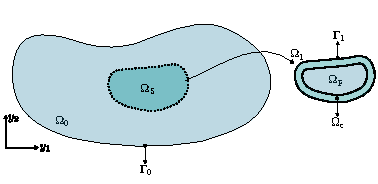
\includegraphics[scale=1.5,trim=0cm 0cm 0cm 0.0cm, clip=true]{Imagens/Cap6/dominioArlequin.pdf}	
	\label{fig:dominioArlequin}
	\legend{Fonte: Elaborada pela autora}
\end{figure}

Dessa forma, o domínio computacional do problema é definido por:

\begin{align}
	\domain = \globalModel + \localModel, 
\end{align}

\noindent e a zona de superposição $\overlappingZone$ é difinida da seguinte forma:

\begin{align}
	\overlappingZone = \globalModel \cap \localModel, \\
	\overlappingZone = \gluingZone \cup \freeZone, \\
	\overlappingZone > 0, 
\end{align}

\noindent sendo  $\freeZone$ a chamada zona livre.

Umas das formas mais comuns de se realizar o acoplamento entre domínios é através de campos de multiplicadores de Lagrange. Uma forma generalizada de representar os operadores de acoplamento, conforme \citeonline{DhiaR:2002}, é:

\begin{align}
	(\lagrangeMultiplier,\Delta \velocity) =  \int_{\gluingZone} k_{0}[\lagrangeMultiplier \cdot \Delta \velocity ] + k_{1}[\straintensor (\lagrangeMultiplier) : \straintensor (\Delta \velocity)] \ \deriv \gluingZone,
\end{align}

\noindent onde $\lagrangeMultiplier$ é o campo de multiplicadores de Lagrange, $\Delta \velocity = \uglobal |_{\gluingZone} - \ulocal |_{\gluingZone}$ é a diferença entre os campos acoplados na zona de colagem. $k_{0}$ e $k_{1}$ são constantes estritamente positivas. 

Quando $k_{0} > 0$ e $k_{1} = 0 $ têm-se o operador de acoplamento $L^{2}$. Esse operador estabelece a continuidade de ordem 0 do campo compatibilizado, o que significada que ele garante, de forma fraca, a continuidade das variáveis ao longo da zona de colagem. Para valores $k_{0} > 0$ e $k_{1} > 0 $ obtêm-se o operador de acoplamento $H^{1}$, estabelecendo continuidade de ordem 1 do campo compatibilizado, garantindo, de forma fraca, a continuidade de uma combinação de variáveis e seu Laplaciano \cite{GuidaultAndBelytschko2007}.

O sucesso do método depende da escolha apropriada dos parâmetros $k_{0}$ e $k_{1}$. Para o acoplamento utilizando $L^{2}$, devido a simplicidade da aplicação da restrição dos campos compatibilizados na zona de colagem, o condicionamento do sistema depende fortemente do valor do parâmetro $k_{0}$, sendo esta uma das razões pela qual a maioria dos trabalhos realizados com o método Arlequin empregam o operador $H^{1}$. A obtenção de parâmetros ótimos para o método pode ser uma tarefa difícil, sendo esse um dos fatores que levaram \citeonline{FernandesEtAll:2020} ao desenvolvimento da técnica RBSAM que será discutida na próxima seção.

A definição do espaço de funções para o multiplicador de Lagrange é muito importante. O método apresenta flexibilidade para usar uma discretização diferente da zona de colagem, entretanto, usualmente se adota um subconjunto do espaço de funções de um dos modelos sobrepostos. A escolha por um modelo ou outro pode conduzir a um maior ou menor acoplamento, sendo a escolha definida em função da aplicação desejada. 

Por fim, para que o método não adicione energia ao sistema, é necessário que seja definida uma função ponderadora, denominada ($\arlequinWF$), que garanta a distribução da energia do sistema ao longo dos modelos sobrepostos. Em geral, essa função é definida da seguinte forma:

\begin{align}
	\begin{cases} \arlequinWFGlobal \in [ka;1] \ em \ \domain, \\ 
	\arlequinWFGlobal = 1 \ em \ \globalModel \textbackslash \localModel,  \\
	\arlequinWFGlobal  = k_a > 0 \ em \ \freeZone, \\
	\arlequinWFGlobal + \arlequinWFLocal = 1 \ em \ \domain,
	\end{cases} \label{eq:funcPondeArleq}
\end{align}

\noindent com $k_a$ uma constante arbitrariamente pequena para o método de Arlequin ser relevante \cite{Dhia:2008}, conforme pode ser observado na \autoref{fig:funcPondArlq}.

\begin{figure}[!htbp]
	\caption{Função Ponderadora}
	\centering 
	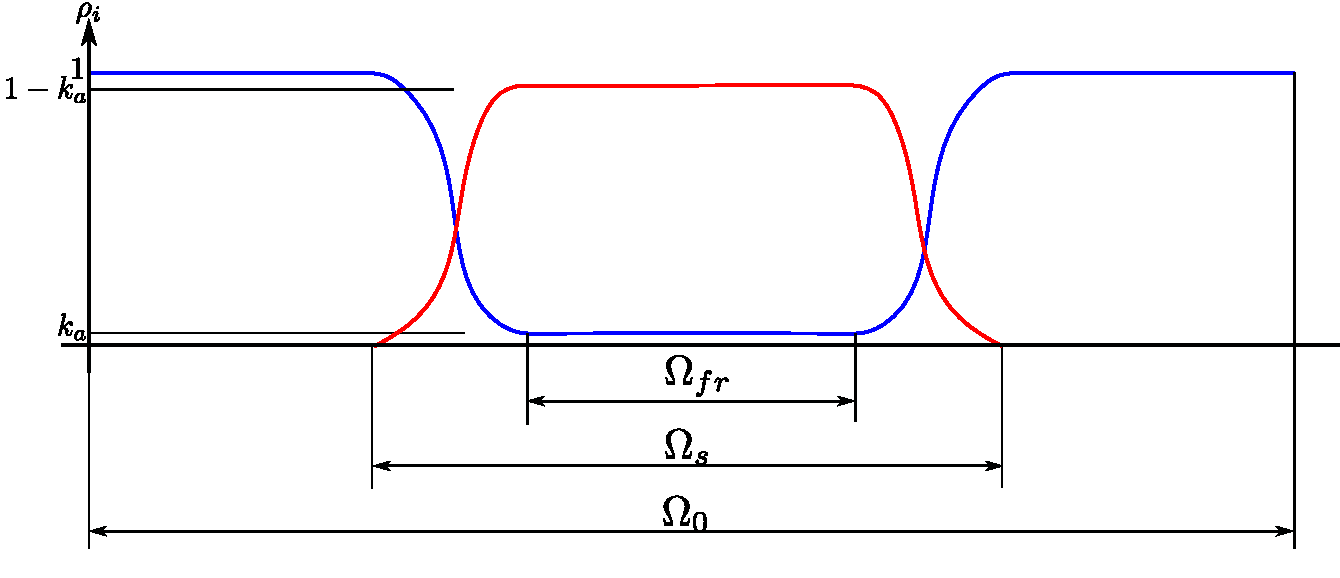
\includegraphics[scale=0.6,trim=0cm 0cm 0cm 0.0cm, clip=true]{Imagens/Cap6/funcPondArlq.pdf}	
	\label{fig:funcPondArlq}
	\legend{Fonte: Elaborada pela autora}
\end{figure}

No caso deste trabalho, adotou-se para $\alpha_0$ e $\alpha_1$ na zona de colagem funções lineares da distância ao contorno $\Gamma_1$, de modo que:... \textcolor{red}{Colocar as funções adotadas em função da distância assinalada...}.

\section{Método Arlequin clássico aplicado a problemas de escoamentos incompressíveis}

O método Arlequin vem sendo aplicado amplamente em diversos trabalhos da mecânica dos sólidos nas últimas décadas. No que diz respeito a materiais incompressíveis, pode-se citar o trabalho de \citeonline{JamondD:2013}, no qual os autores desenvolvem uma técnica para análise empregando elementos do tipo Taylor-Hood, que satisfazem a condição LBB. Essa metodologia é testada também para problemas descritos pelas equações de Stokes.

De acordo com os autores \citeonline{JamondD:2013} a principal dificuldade encontrada para aplicação do método Arlequin no contexto de materiais incompressíveis é que duas restrições devem ser aplicadas concomitantemente: a compatibilização dos campos de interesse na zona de colagem e a condição de incompressibilidade do material nessa mesma região. Os autores apontaram que a imposição da condição de incompressibilidade em ambos os modelos pode gerar problema de redundância, acarretando em um sistema algébrico associado singular.

A solução proposta por \citeonline{JamondD:2013} trabalho foi a aplicação da condição de incompressibilidade em cada ponto do domínio computacional apenas uma vez. A metodologia consiste então em escolher um dos modelos no qual no qual é removida a condição de incompressibilidade dos elementos total ou parcialmente localizados na zona de colagem ($\gluingZone$). Indiferente do modelo eleito para a remoção da condição de incompressibilidade na zona de colagem, na zona livre, a condição de incompressibilidade é removida do modelo global. Deve-se destacar que, no trabalho citado, existem algumas recomendações com relação a estabilidade da metodologiam, como por exemplo, a necessidade de existir pelo menos um elemento global na zona livre. Tal trabalho não explora as possíveis mudanças que acarretariam na estabilidade numérica em caso de sucessivas remoções e inclusões de condição de incompressibilidade no caso de um modelo local móvel.

Por esse motivo, neste trabalho, opta-se pela adoção da formulação estabilizada.
Para a construção do método Arlequin é necessário retornar às equações para um monomodelo apresentadas no Cap. \ref{capitulo:Cap2}, as quais representam a forma fraca estabilizada das equações da quantidade de movimento e da continuidade. Entretanto, será usada inicialmente uma descrição Euleriana das equações.

Considerando os espaços de dimensão finita das funções tentativa que descrevem a velocidade ($\uArlequinSolution$) e a pressão ($\pArlequinSolution$), bem como seus respectivos espaços de funções testes $\uArlequinTest$ e $\pArlequinTest$, com $i = 0,1$ indicando o índice do modelo, definidos como:

\begin{align}
	\uArlequinSolution = \left\{\velocity_{i}^{h} \left . \right| \velocity_{i}^{h} \left(\cdot,t\right) \in (H^{1h}\left(\arlqModel\right), \velocity_{i}^{h} = \velocity_{Di}^{h} \textrm { em}  \ \boundary_{Di} \right\}
\end{align}

\begin{align}
	\pArlequinSolution = \left\{\press_{i}^{h} \left . \right| \press_{i}^{h} \left(\cdot\right) \in L^{2h}\left(\arlqModel\right) \right\},
\end{align}

\begin{align}
	\uArlequinTest = \left\{\utest_{i}^{h} \left . \right| \utest_{i}^{h} \left(\cdot\right) \in H^{1h}\left(\arlqModel\right), \utest_{i}^{h} = \vzero  \textrm { em} \ \boundary_{D_i} \right\},
\end{align}

\noindent e

\begin{align}
	\pArlequinTest = \pArlequinSolution.
\end{align}

Analogamente, os espaços das funções tentativa ($\lagSolution$) e teste ($\lagTest$) para o campo dos multiplicadores de Lagrange ($\lagrangeMultiplier$) são definidos como:

\begin{align}
	\lagSolution = \left\{ \lagrangeMultiplier^{h} \,\middle|\, \lagrangeMultiplier^{h}(\cdot) \in H^{1h}(\gluingZone) \right\}
\end{align}

\begin{align}
	\lagTest = \lagSolution.
\end{align}

A aplicação do operador de acoplamento $L^{2}$ à formulação clássica Arlequin consiste em, dados os espaços tentativa e teste apresentados nas equações anteriores, encontrar $(\uglobalh,\pglobalh,\ulocalh,\plocalh,\lagrangeMultiplierh)$ $\in$ $\uGlobalSolution \times \pGlobalSolution \times \uLocalSolution \times \pLocalSolution \times \lagSolution$ de maneira que  $\forall$ $\wglobalh \in \uGlobalTest$, $\qglobalh \in \pGlobalTest$, $\wlocalh \in \uLocalTest$, $\qlocalh \in \pLocalTest$, e $\forall$ $\lagrangeMultiplierWFh \in \lagTest$:

\begin{align}
	\begin{split}
		&\int_{\globalModel} \arlequinWFGlobal \density \wglobalh \cdot \frac{\partial\uglobalh}{\partial t} \deriv \globalModel +
		\int_{\globalModel} \arlequinWFGlobal \density \wglobalh \cdot  \left(\uglobalh \cdot \gradient \right) \uglobalh \deriv \globalModel  \\ 
		&\quad+	
		\int_{\globalModel} \arlequinWFGlobal \straintensor \left(\wglobalh\right) : \stressTensor \left(\uglobalh,\pglobalh\right)\ \deriv \globalModel \\
		&\quad+ \sum_{e=1}^{\nel} \int_{\domainE} \SUPG  \left(\left(\uglobalh \cdot \gradient \right) \wglobalh\right) \cdot \resMomGlobal\left(\uglobalh,\pglobalh \right)\  \deriv \globalModel \\ 
		&\quad+\sum_{e=1}^{\nel} \int_{\domainE} \LSIC \divergence \cdot \wglobalh \resPreGlobal 
		 \left(\uglobalh\right)\  \deriv \globalModel 
		 + \chi_{0} \int_{\gluingZone} \wglobalh \cdot \lagrangeMultiplierh \deriv \gluingZone   \\ 
		 &\quad = \int_{\globalModel} \arlequinWFGlobal \density \wglobalh \cdot  \globalsbodyforceh \deriv \globalModel + \int_{\globalBoundaryN} \arlequinWFGlobal \wglobalh  \cdot \globalSurfaceLoadh\ \deriv \globalBoundaryN,
		\label{eq:QM_forma_fraca_0}
	\end{split}
\end{align}

\begin{align}
	\begin{split}
		&	\int_{\globalModel} \arlequinWFGlobal \qglobalh \divergence \cdot \uglobalh \ \deriv \globalModel +
\sum_{e=1}^{\nel} \int_{\domainE} \PSPG \left(\frac{\gradient \qglobalh}{\density}\right) \cdot \resMomGlobal\left(\uglobalh,\pglobalh\right) \  \deriv \globalModel,
		\label{eq:C_forma_fraca_0}
	\end{split}
\end{align}

\begin{align}
	\begin{split}
		&\int_{\localModel} \arlequinWFLocal \density \wlocalh \cdot \frac{\partial\ulocalh}{\partial t} \deriv \localModel +
		\int_{\localModel} \arlequinWFLocal \density \wlocalh \cdot  \left(\ulocalh \cdot \gradient \right)\ulocalh \deriv \localModel  \\ 
		&\quad+	
		\int_{\localModel} \arlequinWFLocal \straintensor \left(\wlocalh\right) : \stressTensor \left(\ulocalh,\plocalh\right)\ \deriv \localModel 
		\\ 
		&\quad+ \sum_{e=1}^{\nel} \int_{\domainE} \SUPG  \left( \right(\ulocalh \cdot \gradient \left) \wlocalh\right) \cdot \resMomLocal\left(\ulocalh,\plocalh \right)\  \deriv \localModel \\ 
		&\quad+\sum_{e=1}^{\nel} \int_{\domainE} \LSIC \divergence \cdot \wlocalh \resPreLocal
		\left(\ulocalh\right)\  \deriv \localModel 
		\quad+ \chi_{1} \int_{\gluingZone} \wlocalh \cdot \lagrangeMultiplierh \deriv \gluingZone  \\
		&\quad= \int_{\localModel} \arlequinWFLocal \density \wlocalh \cdot  \localsbodyforceh \deriv \localModel + \int_{\localBoundaryN} \arlequinWFLocal \wlocalh \cdot \localSurfaceLoadh\ \deriv \localBoundaryN,
		\label{eq:QM_forma_fraca_1}
	\end{split}
\end{align}

\begin{align}
	\begin{split}
		&	\int_{\localModel} \arlequinWFLocal \qlocalh \divergence \cdot \ulocalh \ \deriv \localModel +
		\sum_{e=1}^{\nel} \int_{\domainE} \PSPG \left(\frac{\gradient \qlocalh}{\density}\right) \cdot \resMomLocal \left(\ulocalh,\plocalh\right) \  \deriv \localModel = 0,
		\label{eq:C_forma_fraca_1}
	\end{split}
\end{align}

\begin{align}
	\int_{\gluingZone}  \lagrangeMultiplierWFh  \cdot \left(\uglobalh - \ulocalh \right) \ \deriv \gluingZone = 0, 
		\label{eq:lag_acopl}
\end{align}

\noindent onde $\resMomI$ e ${\resPreI}$ são os resíduos da equação da quantidade de movimento e da equação da continuidade, com $i=0,1$, respectivamente, dados por:

\begin{align}
	\resMomI \left(\uArlqi,\pArlqi,\lagrangeMultiplierh \right)&=\arlequinWFi \density\left(\frac{\partial\uArlqi}{\partial t}+ \left( \uArlqi \cdot \gradient \right) \uArlqi - \sbodyforce_i^{h}\right) - \arlequinWFi \divergence \cdot \stressTensor\left(\uArlqi,\pArlqi\right)+ \chi_{i} \lagrangeMultiplierh \label{eq:res_QM_i},
\end{align}

\noindent

\begin{align}
	\resPreI\left(\uArlqi\right)&= \arlequinWFi \divergence \cdot \uArlqi \label{eq:res_C_i}, 
\end{align}

\noindent com $\chi_{i}$ descrito da maneira que se segue:

\begin{align}
	\chi_{i} = \begin{cases} (-1)^{i} \ se \ \pos \in \gluingZone \\
			   0 \ se \ \pos \notin \gluingZone. \end{cases}						. 
\end{align}

O problema descrito pelas equações \ref{eq:QM_forma_fraca_0} à \ref{eq:lag_acopl} é à versão clássica do método de Arlequin para o problema de Navier-Stokes estabilizado pela técnica PSPG/SUPG. Matematicamente trata-se de um problema de ponto de sela decorrente de uma formulação mista. Entretanto, desde que a condição LBB seja satisfeita, existe solução para o problema e ela é única. 

Em \citeonline{GuidaultAndBelytschko2007} pode-se encontrar uma vasta análise matemática acerca das questões relacionadas com estabilidade, convergência e relevância do método. Os autores relatam, por exemplo, a necessidade de emprego de funções ponderadoras contínuas quando utilizado o operador de acoplamento $L^{2}$, o que não ocorre com o operador $H^{1}$. Além disso,  os autores destacam que espaços muito refinados para os multiplicadores de Lagrange podem levar a uma solução não convergente, independente do tipo de operador de acoplamento. Esse problema ocorre devido à forte dependência da discretização do modelo global na solução.

O problema descrito no método Arlequin clássico é análogo a formulação mista em elementos finitos para escoamentos incompressíveis, que limita a escolha das funções aproximadoras para o campo de velocidade e pressão. No caso da mecânica dos fluidos, conforme apresentado no Cap. \ref{capitulo:Cap2}, uma forma de superar as restrições LBB é o uso de métodos estabilizados como o PSPG. Seguindo essa mesma filosofia,  \citeonline{FernandesEtAll:2020} introduzem uma técnica de estabilização consistente que será apresentada na seguinte seção. 

\section{Método Arlequin estabilizado aplicado à problemas de escoamentos incompressíveis}

Com intuito de superar a condição LBB para o método Arlequin, \citeonline{FernandesEtAll:2020} desenvolvem uma técnica de estabilização consistente baseada em resíduo. Para isso, introduz-se uma parcela adicional à equação dos campos de multiplicadores de Lagrange, que leva em conta o gradiente de $\lagrangeMultiplierWFh$ e o resíduo da equação da quantidade de movimento:

\begin{align}
	\sum_{e=1}^{\nel} \int_{\domainE_{c}} \frac{\tauArlequinGlobal}{\rho} \gradient \lagrangeMultiplierWFh : \gradient \resMomGlobal\left(\uglobalh,\pglobalh \right) \ \deriv \gluingZone - 
	\sum_{e=1}^{\nel} \int_{\domainE_{c}} \frac{\tauArlequinLocal}{\rho} \gradient \lagrangeMultiplierWFh : \gradient \resMomLocal\left(\ulocalh,\plocalh \right) \ \deriv \gluingZone,
\end{align}

\noindent sendo $\tauArlequinGlobal$ e $\tauArlequinLocal$ parâmetros de estabilização, respectivamente da malha global e local. A obtenção destes parâmetros será abordada na subseção seguinte. 

Dessa forma, pode-se definir a solução do problema de Navier-Stokes para escoamentos incompressíveis utilizando a técnica de Arlequin estabilizada da seguinte forma: Encontrar $(\uglobalh,\pglobalh,\ulocalh,\plocalh,\lagrangeMultiplierh)$ $\in$ $\uGlobalSolution \times \pGlobalSolution \times \uLocalSolution \times \pLocalSolution \times \lagSolution$ de maneira que  $\forall$ $\wglobalh \in \uGlobalTest$, $\qglobalh \in \pGlobalTest$, $\wlocalh \in \uLocalTest$, $\qlocalh \in \pLocalTest$,   e $\forall$ $\lagrangeMultiplierWFh \in \lagTest$:

\begin{align}
	\begin{split}
		&\int_{\globalModel} \arlequinWFGlobal \density \wglobalh \cdot \frac{\partial\uglobalh}{\partial t} \deriv \globalModel +
		\int_{\globalModel} \arlequinWFGlobal \density \wglobalh \cdot  \left(\uglobalh \cdot \gradient \right) \uglobalh \deriv \globalModel  \\ 
		&\quad+	
		\int_{\globalModel} \arlequinWFGlobal \straintensor \left(\wglobalh\right) : \stressTensor \left(\uglobalh,\pglobalh\right)\ \deriv \globalModel \\
		&\quad+ \sum_{e=1}^{\nel} \int_{\domainE} \SUPG  \left(\left(\uglobalh \cdot \gradient \right) \wglobalh\right) \cdot \resMomGlobal\left(\uglobalh,\pglobalh \right)\  \deriv \globalModel \\ 
		&\quad+\sum_{e=1}^{\nel} \int_{\domainE} \LSIC \divergence \cdot \wglobalh \resPreGlobal 
		\left(\uglobalh\right)\  \deriv \globalModel 
		+ \chi_{0} \int_{\gluingZone} \wglobalh \cdot \lagrangeMultiplierh \deriv \gluingZone   \\ 
		&\quad = \int_{\globalModel} \arlequinWFGlobal \density \wglobalh \cdot  \globalsbodyforceh \deriv \globalModel + \int_{\globalBoundaryN} \arlequinWFGlobal \wglobalh  \cdot \globalSurfaceLoadh\ \deriv \globalBoundaryN,
		\label{eq:QM_forma_fraca_0_atu}
	\end{split}
\end{align}

\begin{align}
	\begin{split}
		&	\int_{\globalModel} \arlequinWFGlobal \qglobalh \divergence \cdot \uglobalh \ \deriv \globalModel +
		\sum_{e=1}^{\nel} \int_{\domainE} \PSPG \left(\frac{\gradient \qglobalh}{\density}\right) \cdot \resMomGlobal\left(\uglobalh,\pglobalh\right) \  \deriv \globalModel,
		\label{eq:C_forma_fraca_0_atu}
	\end{split}
\end{align}

\begin{align}
	\begin{split}
		&\int_{\localModel} \arlequinWFLocal \density \wlocalh \cdot \frac{\partial\ulocalh}{\partial t} \deriv \localModel +
		\int_{\localModel} \arlequinWFLocal \density \wlocalh \cdot  \left(\ulocalh \cdot \gradient \right)\ulocalh \deriv \localModel  \\ 
		&\quad+	
		\int_{\localModel} \arlequinWFLocal \straintensor \left(\wlocalh\right) : \stressTensor \left(\ulocalh,\plocalh\right)\ \deriv \localModel 
		\\ 
		&\quad+ \sum_{e=1}^{\nel} \int_{\domainE} \SUPG  \left( \right(\ulocalh \cdot \gradient \left) \wlocalh\right) \cdot \resMomLocal\left(\ulocalh,\plocalh \right)\  \deriv \localModel \\ 
		&\quad+\sum_{e=1}^{\nel} \int_{\domainE} \LSIC \divergence \cdot \wlocalh \resPreLocal
		\left(\ulocalh\right)\  \deriv \localModel 
		\quad+ \chi_{1} \int_{\gluingZone} \wlocalh \cdot \lagrangeMultiplierh \deriv \gluingZone  \\
		&\quad= \int_{\localModel} \arlequinWFLocal \density \wlocalh \cdot  \localsbodyforceh \deriv \localModel + \int_{\localBoundaryN} \arlequinWFLocal \wlocalh \cdot \localSurfaceLoadh\ \deriv \localBoundaryN,
		\label{eq:QM_forma_fraca_1_atu}
	\end{split}
\end{align}

\begin{align}
	\begin{split}
		&	\int_{\localModel} \arlequinWFLocal \qlocalh \divergence \cdot \ulocalh \ \deriv \localModel +
		\sum_{e=1}^{\nel} \int_{\domainE} \PSPG \left(\frac{\gradient \qlocalh}{\density}\right) \cdot \resMomLocal \left(\ulocalh,\plocalh\right) \  \deriv \localModel = 0,
		\label{eq:C_forma_fraca_1_atu}
	\end{split}
\end{align}

\begin{align}
	\begin{split}
	&\int_{\gluingZone}  \lagrangeMultiplierWFh  \cdot \left(\uglobalh - \ulocalh \right) \ \deriv \gluingZone + \sum_{e=1}^{\nel} \int_{\domainE_{c}} \frac{\tauArlequinGlobal}{\rho} \gradient \lagrangeMultiplierWFh : \gradient \resMomGlobal\left(\uglobalh,\pglobalh\right) \ \deriv \gluingZone  \\
	&\quad-\sum_{e=1}^{\nel} \int_{\domainE_{c}} \frac{\tauArlequinLocal}{\rho} \gradient \lagrangeMultiplierWFh : \gradient \resMomLocal \ \deriv \gluingZone = 0,
	\label{eq:lag_acopl_tARLQ}
\end{split}
\end{align}

\noindent com os resíduos $\resMomI$ e $\resPreI$ escritos conforme as \autoref{eq:res_QM_i} e Eq .\ref{eq:res_C_i}.

O sistema resultante pode ser reescrito em notação matricial como:

\begin{align}
	\begin{bmatrix}
		\mathbf{K}_{0} & \vzero & \mathbf{\hat{L}}_{0} \\
		\vzero & \mathbf{K}_{1} & - \mathbf{\hat{L}}_{1} \\
		\mathbf{L}_{0}^{T} & -\mathbf{L}_{1}^{T} & \mathbf{E}
	\end{bmatrix}
	\begin{bmatrix}
		\mathbf{\bar{U}}_{0} \\
		\mathbf{\bar{U}}_{1} \\
		\LagrangeMultiplier
	\end{bmatrix}
	&=
	\begin{bmatrix}
		\mathbf{F}_0 \\
		\mathbf{F}_1 \\
		\mathbf{F}_{\LagrangeMultiplier}
	\end{bmatrix}.
	\label{eq:sistema_result_ArlqRBSAM}
\end{align}	

Considerando $i=0,1$ designando os modelos global e local respectivamente, têm-se a definição dos termos da \autoref{eq:sistema_result_ArlqRBSAM} como: $\mathbf{K}_{i}$ é uma matriz que representa os termos provenientes das matrizes referentes as equações da quantidade de movimento e da continuidade para o modelo $i$; $\mathbf{\hat{L}}_{i}$ matriz que representa os termos de acoplamento do modelo $i$; $\mathbf{L}_{i}^{T}$ matriz procedente dos termos da equação de restrição e de componentes da estabilização RBSAM do modelo $i$; $\mathbf{E}$ apresenta termos oriundos da estabilização RBSAM; $\mathbf{\bar{U}}_{i}$ representa os vetores nodais dos graus de liberdade respectivos a velocidade e pressão do modelo $i$; $\LagrangeMultiplier$ representa os graus de liberdade respectivos aos multiplicadores de Lagrange; $\mathbf{F}_i$ representa os vetores provenientes das equações da quantidade de movimento e da continuidade para o modelo $i$; $\mathbf{F}_{\LagrangeMultiplier}$ representa os termos vetoriais advindos da estabilização RBSAM. 

Note que na estabilização Arlequin baseada no resíduo (RBSAM) não existem elementos zeros na diagonal da matriz, diferente do mesmo problema na formulação clássica Arlequin. No trabalho de \citeonline{FernandesEtAll:2020} pode-se encontrar a análise de estabilidade dessa técnica e testes numéricos que avaliam o condicionamento do sistema algébrico e a convergência do método.

O problema de Arlequin não linear apresentado nas equações: \autoref{eq:QM_forma_fraca_0_atu} à \ref{eq:lag_acopl_tARLQ} pode ser reescrito em sua forma semi-discreta residual para $i=0,1$, da seguinte maneira:

\begin{align}
	\begin{split}
		\NNSMArlq =\; & \int_{\arlqModel} \arlequinWFi \density\, \wArlqi \cdot \frac{\partial\uArlqi}{\partial t} \, \deriv \arlqModel 
		+ \int_{\arlqModel} \arlequinWFi \density\, \wArlqi \cdot \left( \uArlqi \cdot \gradient \right)\uArlqi \, \deriv \arlqModel  \\ 
		&+ \int_{\arlqModel} \arlequinWFi\, \straintensor \left(\wArlqi\right) : \stressTensor \left(\uArlqi,\pArlqi\right) \, \deriv \arlqModel 
		\\ 
		&+ \sum_{e=1}^{\nel} \int_{\domainE} \SUPG\, \left( \left( \uArlqi \cdot \gradient \right)\wArlqi \right) \cdot \resMomI \left(\uArlqi,\pArlqi \right) \, \deriv \arlqModel \\ 
		&+ \sum_{e=1}^{\nel} \int_{\domainE} \LSIC\, \divergence \cdot \wArlqi\, \resPreI \left(\uArlqi\right) \, \deriv \arlqModel 
		+ \chi_{i} \int_{\gluingZone} \wArlqi \cdot \lagrangeMultiplier^{h} \, \deriv \gluingZone \\
		&- \int_{\arlqModel} \arlequinWFi \density\, \wArlqi \cdot \arlqsbodyforceh \, \deriv \arlqModel 
		- \int_{\arlqBoundary} \arlequinWFi\, \wArlqi \cdot \arlqSurfaceLoadh \, \deriv \arlqBoundary
	\end{split}
\end{align}

\begin{align}
	\begin{split}
		&\NNSCArlq = \int_{\arlqModel} \arlequinWFi \qArlqi \divergence \cdot \uArlqi \ \deriv \arlqModel +
		\sum_{e=1}^{\nel} \int_{\domainE} \PSPG \left(\frac{\gradient \qArlqi }{\density}\right) \cdot \resMomI \left(\uArlqi,\pArlqi \right) \  \deriv \arlqModel,
	\end{split}
\end{align}

\begin{align}
	\begin{split}
		&\NNSL = \int_{\gluingZone}  \lagrangeMultiplierWFh  \cdot \left(\uglobalh - \ulocalh \right) \ \deriv \gluingZone + \sum_{e=1}^{\nel} \int_{\domainE_{c}} \frac{\tauArlequinGlobal}{\rho} \gradient \lagrangeMultiplierWFh : \gradient \resMomGlobal\left(\uglobalh,\pglobalh\right) \ \deriv \gluingZone\\
		&\qquad - \sum_{e=1}^{\nel} \int_{\domainE_{c}} \frac{\tauArlequinLocal}{\rho} \gradient \lagrangeMultiplierWFh : \gradient \resMomLocal\left(\ulocalh,\plocalh\right) \ \deriv \gluingZone.
	\end{split}
\end{align}

Considerando $\Acceleration_i$, $\Velocity_i$, $\Press_i$ e $\LagrangeMultiplier$ os vetores nodais dos graus de liberdade respectivos a aceleração, velocidade, pressão e multiplicadores de Lagrange, pode-se escrever o problema semidiscreto da DFC como: Determinar $\Acceleration_0$, $\Velocity_0$, $\Press_0$,$\Acceleration_1$, $\Velocity_1$, $\Press_1$ e $\LagrangeMultiplier$ de maneira que:

\begin{align}
	\NNSMGlobal(\Acceleration_0,\Velocity_0,\Press_0,\LagrangeMultiplier) = \vzero, \label{eq:resid_semi_discr_QM_0}
\end{align}

\begin{align}
	\NNSCGlobal(\Acceleration_0,\Velocity_0,\Press_0,\LagrangeMultiplier) = \vzero, 
\end{align}

\begin{align}
	\NNSMLocal(\Acceleration_1,\Velocity_1,\Press_1,\LagrangeMultiplier) = \vzero,
\end{align}

\begin{align}
	\NNSCLocal(\Acceleration_1,\Velocity_1,\Press_1,\LagrangeMultiplier) = \vzero,
\end{align}

\begin{align}
	\NNSL(\Acceleration_0,\Velocity_0,\Press_0,\Acceleration_1,\Velocity_1,\Press_1,\LagrangeMultiplier) = \vzero. \label{eq:resid_semi_discr_acopla}
\end{align}


\subsection{Parâmetro de estabilização para técnica RBSAM}

No método Arlequin estabilizado, há ainda a necessidade de definição do parâmetro de estabilização $\tauArlequin$, o qual deve possuir valor suficiente para estabilizar os campos de multiplicadores de Lagrange sem, no entanto, comprometer a convergência do método. 

Para a definição de $\tauArlequin$ toma-se como referência os trabalhos de \citeonline{TezduyarO:2000} e \citeonline{TezduyarS:2003} nos quais se apresenta uma vasta quantidade de informação a cerca das técnicas para obtenção dos parâmetros de estabilização das equações da DFC ($\SUPG$, $\PSPG$, $\LSIC$). 
 
Para um bom condicionamento do sistema, busca-se que os termos estabilizantes adicionados possuam magnitude próxima aos termos da equação de acoplamento. Assim, calcula-se $\tauArlequini$ por meio da relação entre normas de vetores que compõem a formulação por elementos finitos, definindo-se um parâmetro para cada um dos modelos por meio de:

\begin{align}
	\tauArlequini = \left(\frac{1}{\left(\tau_{A_i}\right)^{2}} + \frac{1}{\left(\tau_{B_i}\right)^{2}} +  \frac{1}{\left(\tau_{C_i}\right)^{2}} + 
	\frac{1}{\left(\tau_{D_i}\right)^{2}} +
	\frac{1}{\left(\tau_{E_i}\right)^{2}}
	\right)^{-\frac{1}{2}},
\end{align}

\noindent com $i=0,1$ definindo os modelos global e local, respectivamente e:

\begin{align}
	\tau_{A_{i}} = \left(\frac{1}{\left(\tau_{A_i^{0}}\right)^{2} + \left(\tau_{A_i^{1}}\right)^{2}} \right)^{-\frac{1}{2}}, \label{eq:tAi}
\end{align}

\begin{align}
	\tau_{B_{i}} = \left(\frac{1}{\left(\tau_{B_i^{0}}\right)^{2} + \left(\tau_{B_i^{1}}\right)^{2}} \right)^{-\frac{1}{2}},
\end{align}

\begin{align}
	\tau_{C_{i}} = \left(\frac{1}{\left(\tau_{C_i^{0}}\right)^{2} + \left(\tau_{C_i^{1}}\right)^{2}} \right)^{-\frac{1}{2}},
\end{align}

\begin{align}
	\tau_{D_{i}} = \left(\frac{1}{\left(\tau_{D_i^{0}}\right)^{2} + \left(\tau_{D_i^{1}}\right)^{2}} \right)^{-\frac{1}{2}},
\end{align}

\begin{align}
	\tau_{E_{i}} = \left(\frac{1}{\left(\tau_{E_i^{0}}\right)^{2} + \left(\tau_{E_i^{1}}\right)^{2}} \right)^{-\frac{1}{2}},\label{eq:tEi}
\end{align}

\noindent sendo as variáveis das equações \refeq{eq:tAi} a \refeq{eq:tEi} as seguintes normas vetoriais:

\begin{align}
	\tau_{A_i^{0}} = \frac{|| \mathbf{M}_{\lambda_0} || }{||\mathbf{t}_{i} ||}; \ \ \ \ \  & \tau_{A_i^{1}} = \frac{|| \mathbf{M}_{\lambda_1} || }{||\mathbf{t}_{i} ||};
\end{align}

\begin{align}
	\tau_{B_i^{0}} = \frac{|| \mathbf{M}_{\lambda_0} || }{||\mathbf{j}_{i} ||}; \ \ \ \ \  &  \tau_{B_i^{1}} = \frac{|| \mathbf{M}_{\lambda_1} || }{||\mathbf{j}_{i} ||}; 
\end{align}

\begin{align}
	\tau_{C_i^{0}} = \frac{|| \mathbf{M}_{\lambda_0} || }{||\mathbf{k}_{i} ||}; \ \ \ \ \  & \tau_{C_i^{1}} = \frac{|| \mathbf{M}_{\lambda_1} || }{||\mathbf{k}_{i} ||};
\end{align}

\begin{align}
	\tau_{D_i^{0}} = \frac{|| \mathbf{M}_{\lambda_0} || }{||\mathbf{p}_{i} ||}; \ \ \ \ \  & \tau_{D_i^{1}} = \frac{|| \mathbf{M}_{\lambda_1} || }{||\mathbf{p}_{i} ||}; 
\end{align}

\begin{align}
	\tau_{E_i^{0}} = \frac{|| \mathbf{M}_{\lambda_0} || }{||\mathbf{\Gamma}_{i} ||}; \ \ \ \ \  & \tau_{E_i^{1}} = \frac{|| \mathbf{M}_{\lambda_1} || }{||\mathbf{\Gamma}_{i} ||};
\end{align}

Por fim, os vetores em questão, são definidos através das seguintes relações:

\begin{align}
	\mathbf{M}_{\lambda_0} = \int_{\gluingZone} \shapef_{k} \cdot \uglobalh \deriv \gluingZone,
\end{align}

\begin{align}
	\mathbf{M}_{\lambda_1} = - \int_{\gluingZone} \shapef_{k} \cdot \ulocalh \deriv \gluingZone,
\end{align}

\begin{align}
	\mathbf{t}_{i} = \int_{\gluingZone} \gradient \shapef_{k} : \arlequinWFi \gradient \left( \left( \uArlqi \cdot  \gradient \right) \uArlqi \right)  \deriv \gluingZone,
\end{align}

\begin{align}
	\mathbf{j}_{i} = \int_{\gluingZone} \gradient \shapef_{k} :  \arlequinWFi \gradient \left(\frac{\partial\uArlqi}{\partial t}  \right)  \deriv \gluingZone,
\end{align}

\begin{align}
	\mathbf{k}_{i} = \int_{\gluingZone} \gradient^{2} \shapef_{k} : \arlequinWFi 2 \viscosity \divergence \cdot \straintensor \left(\uArlqi\right)    \deriv \gluingZone,
\end{align}

\begin{align}
	\mathbf{p}_{i} = \int_{\gluingZone} \gradient \shapef_{k} : \arlequinWFi \gradient \left(-\gradient \pArlqi \right)    \deriv \gluingZone,
\end{align}

\begin{align}
	\mathbf{\Gamma}_{i} = \int_{\gluingZone} \gradient \shapef_{k} : \gradient \left(\chi (i) \lagrangeMultiplierh\right)    \deriv \gluingZone,
\end{align}

\noindent com $k$ representando o índice dos graus de liberdade do campo de multiplicadores de Lagrange.

\subsection{Integração Temporal e processo de solução}

Quanto ao procedimento de integração temporal, utiliza-se o método $\alpha$-generalizado conforme a metodologia apresentada na \autoref{capitulo:Cap2:IntegTemp}, para a solução do sistema de equações não lineares composto por \autoref{eq:resid_semi_discr_QM_0} a \autoref{eq:resid_semi_discr_acopla}, utiliza-se o método de Newton-Raphson. A solução resulta em uma etapa preditiva e outra iterativa corretiva.

Na etapa preditiva, conhecida a solução em um passo de tempo $n$, prediz-se a solução no passo seguinte ($n+1$) através das seguintes relações:

\begin{align}
	\Acceleration_{0(n+1)}^{0} = \frac{\gamma-1}{\gamma}\Acceleration_{0(n)} \label{eq:pred_acel_0},
\end{align}

\begin{align}
	\Velocity_{0(n+1)}^{0} = \Velocity_{0(n)}, \label{eq:pred_vel_0}
\end{align}

\begin{align}
	\Press_{0(n+1)}^{0} = \Press_{0(n)},\label{eq:pred_press_0}
\end{align}

\begin{align}
	\Acceleration_{1(n+1)}^{0} = \frac{\gamma-1}{\gamma}\Acceleration_{1(n)} \label{eq:pred_acel_1},
\end{align}

\begin{align}
	\Velocity_{1(n+1)}^{0} = \Velocity_{1(n)}, \label{eq:pred_vel_1}
\end{align}

\begin{align}
	\Press_{1(n+1)}^{0} = \Press_{1(n)},\label{eq:pred_press_1}
\end{align}

\begin{align}
	\LagrangeMultiplier_{(n+1)}^{0} = \LagrangeMultiplier_{(n)},\label{eq:pred_lag_mult}
\end{align}

\noindent onde o superíndice $0$ representa a iteração de número zero, enquanto que os subíndices $0$ e $1$ representam as variáveis do modelo global e local, respectivamente.

A etapa iterativa corretiva é constituída por três fases. A fase 1 consiste em determinar os valores no instante intermediário para as variáveis nodais na iteração $i$ por meio de:

\begin{align}
	\Acceleration_{0({n+\alpham})}^{i} = \Acceleration_{0(n)} + \alpham \left( \Acceleration_{0(n+1)}^{i} - \Acceleration_{0(n)} \right), \label{eq:inter_acel_0}\\
	\Velocity_{0(n+\alphaf)}^{i} = \Velocity_{0(n)} + \alphaf \left( \Velocity_{0(n+1)}^{i} - \Velocity_{0(n)} \right), \label{eq:inter_vel_0}\\
	\Press_{0(n+1)}^{i} = \Press_{0(n+1)}^{i}, \label{eq:inter_press_0} \\
	\Acceleration_{1(n+\alpham)}^{i} = \Acceleration_{1(n)} + \alpham \left( \Acceleration_{1(n+1)}^{i} - \Acceleration_{1(n)} \right), \label{eq:inter_acel_1}\\
	\Velocity_{1(n+\alphaf)}^{i} = \Velocity_{1(n)} + \alphaf \left( \Velocity_{1(n+1)}^{i} - \Velocity_{1(n)} \right), \label{eq:inter_vel_1}\\
	\Press_{1(n+1)}^{i} = \Press_{1(n+1)}^{i},\label{eq:inter_press_1} \\
	\LagrangeMultiplier_{(n+1)}^{i} = \LagrangeMultiplier_{(n+1)}^{i}. \label{eq:inter_lag_mult}
\end{align}

Na fase 2, com os valores intermediários das variáveis nodais resolve-se o sistema resultante da linearização das equações \autoref{eq:resid_semi_discr_QM_0} à \autoref{eq:resid_semi_discr_acopla} com respeito às variáveis de interesse $\Acceleration_{0(n+1)}$, $\Press_{0(n+1)}$,  $\Acceleration_{1(n+1)}$, $\Press_{1(n+1)}$ e $\LagrangeMultiplier_{(n+1)}$, calculando-se uma correção para essas variáveis:

\begin{align}
	\begin{bmatrix}
		\frac{\partial\NNSMGlobal}{\partial\Acceleration_{0(n+1)}^{i}} & \frac{\partial\NNSMGlobal}{\partial\Press_{0(n+1)}^{i}} & \vzero & \vzero & \frac{\partial\NNSMGlobal}{\partial\LagrangeMultiplier_{(n+1)}^{i}} \\
		\frac{\partial\NNSCGlobal}{\partial\Acceleration_{0(n+1)}^{i}} & \frac{\partial\NNSCGlobal}{\partial\Press_{0(n+1)}^{i}} & \vzero & \vzero & \frac{\partial\NNSCGlobal}{\partial\LagrangeMultiplier_{(n+1)}^{i}} \\
		 \vzero & \vzero & \frac{\partial\NNSMLocal}{\partial\Acceleration_{1(n+1)}^{i}} & \frac{\partial\NNSMLocal}{\partial\Press_{1(n+1)}^{i}} & \frac{\partial\NNSMLocal}{\partial\LagrangeMultiplier_{(n+1)}^{i}} \\
		 \vzero & \vzero & \frac{\partial\NNSCLocal}{\partial\Acceleration_{1(n+1)}^{i}} & \frac{\partial\NNSCLocal}{\partial\Press_{1(n+1)}^{i}} & \frac{\partial\NNSCLocal}{\partial\LagrangeMultiplier_{(n+1)}^{i}} \\
		  \frac{\partial\NNSL}{\partial\Acceleration_{0(n+1)}^{i}} & \frac{\partial\NNSL}{\partial\Press_{0(n+1)}^{i}} & \frac{\partial\NNSL}{\partial\Acceleration_{1(n+1)}^{i}} & \frac{\partial\NNSL}{\partial\Press_{1(n+1)}^{i}} & \frac{\partial\NNSL}{\partial\LagrangeMultiplier_{(n+1)}^{i}}
	\end{bmatrix}
	\begin{bmatrix}
		\Delta\Acceleration_{0(n+1)}^{i} \\
		\Delta\Press_{0(n+1)}^{i} \\
		\Delta\Acceleration_{1(n+1)}^{i} \\
		\Delta\Press_{1(n+1)}^{i} \\
		\LagrangeMultiplier_{(n+1)}^{i}
	\end{bmatrix}
	&=
	\begin{bmatrix}
		-\NNSMGlobal \\
		-\NNSCGlobal \\
		-\NNSMLocal \\
		-\NNSCLocal \\
		-\NNSL
	\end{bmatrix}
	\label{eq:sistema_linear_Arlq}
\end{align}	

Atualiza-se então, na fase 3, as variáveis incóginitas por meio de:

\begin{align}
	\Acceleration_{0(n+1)}^{i+1} = \Acceleration_{0(n+1)}^{i} + \Delta\Acceleration_{0(n+1)}^{i}, \label{eq:atu_acel_0} \\ 
	\Velocity_{0(n+1)}^{i+1} = \Velocity_{0(n+1)}^{i} + \gamma \Delta t \Delta\Velocity_{0(n+1)}^{i},\label{eq:atu_vel_0}\\
	\Press_{0(n+1)}^{i+1} = \Press_{0(n+1)}^{i} + \Delta\Press_{0(n+1)}^{i}, \label{eq:atu_press_0} \\
	\Acceleration_{1(n+1)}^{i+1} = \Acceleration_{1(n+1)}^{i} + \Delta\Acceleration_{1(n+1)}^{i}, \label{eq:atu_acel_1} \\ 
	\Velocity_{1(n+1)}^{i+1} = \Velocity_{1(n+1)}^{i} + \gamma \Delta t \Delta\Velocity_{1(n+1)}^{i},\label{eq:atu_vel_1}\\
	\Press_{1(n+1)}^{i+1} = \Press_{0(n+1)}^{i} + \Delta\Press_{1(n+1)}^{i}, \label{eq:atu_press_1} \\
	\LagrangeMultiplier_{1(n+1)}^{i+1} = \LagrangeMultiplier_{0(n+1)}^{i} + \Delta\LagrangeMultiplier_{1(n+1)}^{i}. \label{eq:atu_lag_mult}
\end{align}

Na utilização do método $\alpha$-generalizado as integrais das equações são avaliadas no instante $t = t_{n+\alphaf}$. As relações entre velocidade, aceleração, e os parâmetros utilizados pelo método podem ser consultados na \autoref{capitulo:Cap2:IntegTemp}.



\section{Superposição de modelos móveis}

As equações \autoref{eq:QM_forma_fraca_0_atu} à \autoref{eq:lag_acopl_tARLQ} resolvem problemas de escoamentos incompressíveis em uma discretização Euleriana. Entretanto, tem-se como objetivo a movimentação do domínio local do fluido (ver \autoref{fig:dominioArlequinMovel}) para acomodar a movimentação da estrutura nos problemas de IFE, ou para representar o deslocamento de um objeto imerso no escoamento. Nota-se que o modelo global mantém sua geometria inalterada na mudança de passo de tempo, enquanto que o modelo local é movimentado para representar uma nova localização de um objeto imerso. Vale ressaltar que o contorno do domínio do modelo local ($\localBoundary$) é conhecido em $t_n$ e em $t_{n+1}$, e que a zona de superposição $\overlappingZone$ é definida em diferentes posições em cada instante.. Assim, faz-se uso de uma descrição Lagrangiana-Euleriana Arbitrária (ALE) no modelo local ($\localModel$) enquanto que o domínio global ($\globalModel$) mantém-se fixo e com descrição Euleriana. 

Para análise de domínios móveis do tipo Euleriano-ALE, a \autoref{eq:QM_forma_fraca_1_atu} é reescrita, levando-se em consideração as definições apresentadas na \autoref{capitulo:Cap2:ALE}, resultando em:

\begin{align}
	\begin{split}
		&\int_{\localModel} \arlequinWFLocal \density \wlocalh \cdot \left. \frac{\partial\ulocalh}{\partial t} \right|_{\posALE} \deriv \localModel +
		\int_{\localModel} \arlequinWFLocal \density \wlocalh \cdot  \left(\left(\ulocalh - \velocityALEh_{1}\right) \cdot \gradient \ulocalh\right) \deriv \localModel  \\ 
		&\quad+	
		\int_{\localModel} \arlequinWFLocal \straintensor \left(\wlocalh\right) : \stressTensor \left(\ulocalh,\plocalh\right)\ \deriv \localModel 
		\\ 
		&\quad+ \sum_{e=1}^{\nel} \int_{\domainE} \SUPG  \left( \left(\ulocalh - \velocityALEh_{1}\right) \cdot \gradient \wlocalh\right) \cdot \resMomLocal\left(\ulocalh,\plocalh \right)\  \deriv \localModel \\ 
		&\quad+\sum_{e=1}^{\nel} \int_{\domainE} \LSIC \divergence \cdot \wlocalh \resPreLocal
		\left(\ulocalh\right)\  \deriv \localModel \\
		&\quad+  \chi_{1} \int_{\gluingZone} \wlocalh \cdot \lagrangeMultiplierh \deriv \gluingZone  = \int_{\localModel} \arlequinWFLocal \density \wlocalh \cdot  \localsbodyforceh \deriv \localModel + \int_{\localBoundaryN} \arlequinWFLocal \wlocalh \cdot \localSurfaceLoadh\ \deriv \localBoundaryN,
		\label{eq:eq:QM_forma_fraca_1_ALE}
	\end{split}
\end{align}

\noindent enquanto o resíduo apresentado na \autoref{eq:res_QM_i} passa a ser escrito para i = 1, como:

\begin{align}
	\resMomLocal \left(\ulocalh,\plocalh,\lagrangeMultiplierh \right)&=\arlequinWFLocal \density\left(\left. \frac{\partial\ulocalh}{\partial t} \right|_{\posALE}+ \left(\ulocalh - \velocityALEh_{1}\right) \cdot \gradient \ulocalh  - \localsbodyforceh\right) - \arlequinWFLocal \divergence \cdot \stressTensor\left(\ulocalh,\plocalh,\right)+ \chi_{1} \lagrangeMultiplierh \label{eq:res_QM_ALE}.
\end{align}

Além da consideração da descrição ALE para o modelo local, deve-se ressaltar que a função ponderadora $\arlequinWFi$ passa a ser uma variável temporal, ou seja, $\arlequinWFi(t)$, visto que a zona de superposição $\overlappingZone$ é definida em diferentes posições em cada instante de tempo. Dessa forma, a integração temporal utilizando-se o método $\alpha$-generalizado deve considerar essa variação através da seguinte interpolação para o instante intermediário:

\begin{align}
	\arlequinWF_{i(n+\alphaf)} = \arlequinWF_{i(n)} + \alphaf(\arlequinWF_{i(n+1)} - \arlequinWF_{i(n)}).
\end{align}

\begin{figure}[!htbp]
	\caption{Domínio Arlequin móvel}
	\centering 
	{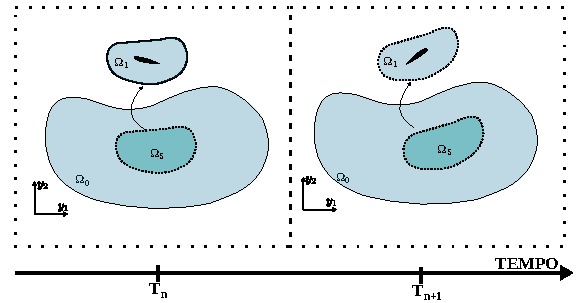
\includegraphics[scale=1.5,trim=0cm 0cm 0cm 0cm, clip=true]{Imagens/Cap6/dominioArlequinMovel.pdf}}	
	\label{fig:dominioArlequinMovel}
	\legend{Fonte: Elaborada pela autora}
\end{figure}

A solução de modelos móveis requer a utilização de uma técnica adequada para movimentação da malha local. A técnica utilizada nesse trabalho toma como base o método MJBS (Mesh-Jacobian Based Stiffening) introduzido por \citeonline{TezduyarBSJ:1992f} e será abordada na  \autoref{capitulo:Cap7:CondAcop:MovMalha}. \textcolor{red}{Não é melhor você colocar que está utilizando a versão da técnica desenvolvida no seu artigo? Afinal, é um caso particular ela.}

O campo dos multiplicadores de Lagrange, neste estudo, é definido do espaço de funções da malha local. Tal escolha ocorre pelo fato de que, mesmo em problemas em que se tenham grandes deslocamentos, a quantidade de elementos locais da zona de superposição permanece inalterada, fazendo com que o sistema algébrico mantenha-se com dimensão constante ao longo do tempo, diminuindo assim, o custo computacional. 

\section{Implementação Computacional}

A implementação desse método envolve a realização de algumas etapas adicionais no início de cada iteração, sendo essas: 1. Determinação de distâncias assinaladas; 2. Determinação da zona de colagem;  3. Determinação da função ponderadora; 4. Encontro de correspondência dos pontos de quadratura do modelo local no modelo global.

A etapa 1 consiste em determinar a distância assinalada com relação ao contorno $\localBoundary$ de todos os pontos (nós para malha de elementos finitos ou pontos de controle para malha isogeométrica) que compõe cada um dos modelos. Na etapa 2, a partir da distância assinalada, são definidos os elementos locais que fazem parte da zona de colagem em função da espessura adotada para essa região, previamente indicada pelo usuário. A função ponderadora para os modelos (etapa 3) é  determinada em função da função distância assinalada e da espessura da zona de colagem de acordo com \autoref{} \textcolor{red}{Colocar equação}. 

Uma das maiores dificuldades da técnica Arlequin diz respeito à integração numérica do operador de acoplamento por demandar integral de funções definidas em modelos distintos. Neste estudo, a integração numérica é definida sobre a malha local, desta forma, durante o pré-processamento de cada iteração para solução do sistema, realiza-se um processo de busca de correspondência (etapa 4) na malha global para cada ponto de integração da malha local, determinando-se o vetor de coordenadas locais e o elemento da malha global correspondente a cada ponto de integração da malha local na zona de colagem.

É importante notar que, antes das etapas 1 a 4, é necessário que a malha local tenha sido atualizada, o que é feito ao final de cada iteração.

O Algoritmo que descreve a implementação computacional é apresentado no Alg. \ref{alg:fluidARLQ}. A implementação computacional e resolução do sistema de equações resultantes ocorreu de forma análoga ao monomodelo descrito na \autoref{capitulo:Cap2:DFCComputationalCode}. O índice $i$ apresentado diz respeito à iteração de Newton-Raphson.

\begin{algorithm}
	\caption{Algoritmo para problemas móveis da DFC utilizando técnica ARLEQUIN RBSAM}
	\label{alg:fluidARLQ}
	\begin{algorithmic}[1]
		\For {o passo de tempo $0$ até \totalTime} 
		\State $i=0$; \textcolor{red}{defina i}
		\State Predição da solução: aplicação da \autoref{eq:pred_acel_0}, \autoref{eq:pred_vel_0}, \autoref{eq:pred_press_0},
		\autoref{eq:pred_acel_1}, \autoref{eq:pred_vel_1}, \autoref{eq:pred_press_1} e \autoref{eq:pred_lag_mult};
		\While{($\epsilon$ < tolerância)}
		\State $i$++;
		\State Cálculo da distância assinalada dos nós e pontos de controle ao contorno $\localBoundary$;
		\State Determinação da zona de colagem $\gluingZone$;
		\State Definição da função de ponderadora de acordo com \autoref{eq:funcPondeArleq};
		\State Busca pela correspondência entre os pontos de integração da malha local na malha global;
		\State Interpolação das variáveis do problema: aplicação da \autoref{eq:inter_acel_0}, \autoref{eq:inter_vel_0}, \autoref{eq:inter_press_0},
		\autoref{eq:inter_acel_1}, \autoref{eq:inter_vel_1}, \autoref{eq:inter_press_1} e \autoref{eq:inter_lag_mult}; 
		\State Cálculo da correção das variáveis do problema: Resolução do sistema apresentado na \autoref{eq:sistema_linear_Arlq};
		\State Atualização da solução: cálculo de acordo com \eqref{eq:atu_acel_0}, \autoref{eq:atu_vel_0}, \autoref{eq:atu_press_0},
		\autoref{eq:atu_acel_1}, \autoref{eq:atu_vel_1}, \autoref{eq:atu_press_1} e \autoref{eq:atu_lag_mult};
		\State Cálculo do erro:
		\begin{align}
			\epsilon =\left\| \NNSMGlobal^{i} + \NNSMLocal^{i}  \right\|_{L^2};
		\end{align}
		\State Movimentação da malha;
		\EndWhile
		\EndFor
	\end{algorithmic}
\end{algorithm}

\section{Exemplos}\label{capitulo:Cap6:Exemplos}

Para a verificação da implementação do método Arlequin estabilizado, dois exemplos amplamente explorados nas bibliografias são simulados. O primeiro exemplo, trata-se de escoamento sobre um aerofólio NACA 0012 fixo, enquanto o segundo, com intuito de verificar o método aplicado a problemas com contornos móveis, trata do mesmo aerofólio NACA 0012, porém com um movimento de arfagem prescrito. 

\parei aqui......

\subsection{Escoamento sobre aerofólio NACA 0012 fixo} \label{capitulo:Cap6:Exemplos:NACA0012}

Para simulação do problema de escoamento sobre um aerofólio NACA 0012, com 1 unidade de corda de dimensão e ângulo de ataque de $10^{\circ}$, utilizou-se o domínio apresentado na \autoref{fig:aerofolio_geometria}. O contorno da entrada de fluxo está localizado a 6 cordas (C) do bordo de ataque do aerofólio, com velocidade de entrada $u_{\infty}$ na direção $y_1$. Os contornos superior e inferior da geometria, com condições de contorno de parede lisa, também estão afastados do aerofólio em 6 unidades de corda. O contorno direito do domínio é localizado a 20 unidades de corda a jusante do bordo de fuga do aerofólio. 

\begin{figure}[!htbp]
	\caption{Aerofólio: Geometria}
	\centering 
	{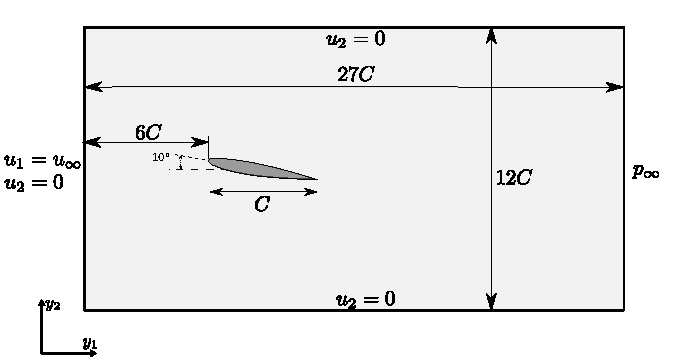
\includegraphics[scale=1.0,trim=0cm 0cm 0cm 0cm, clip=true]{Imagens/Cap6/aerofolio_geometria.pdf}}	
	\label{fig:aerofolio_geometria}
	\legend{Fonte: Elaborada pela autora}
\end{figure}

A análise é realizada para um número de Reynolds ($\Reynolds$) 1000 calculado a partir da dimensão do aerofólio e da velocidade de entrada do escoamento. Foram utilizados ainda como parâmetros de análise: $u_{\infty} = 1,0$,  $\density = 1,0$,  $\timeStep = 0,02$, e $\specRadius = 0,75$.

Para validação da teoria apresentada nesse capítulo, compararam-se os resultados de coeficientes de arrasto e sustentação ao longo do tempo para duas discretizações distintas: 1. Monomodelo; 2. Combinação de duas malhas através do método Arlequin estabilizado.

O monomodelo foi discretizado através de elementos finitos (\autoref{fig:aerofolio_malhaMonoFEM}), com malha constituída de 9240 elementos triangulares quadráticos e 18792 nós. 

\begin{figure}[!htbp]
	\caption{Aerofólio: Malha Monomodelo (MEF)}
	\centering 
	{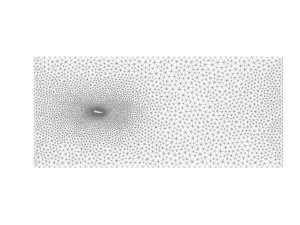
\includegraphics[scale=2.5,trim=0cm 0.9cm 0cm 0.8cm, clip=true]{Imagens/Cap6/aerofolio_malhaMonoFEM.pdf}}	
	\label{fig:aerofolio_malhaMonoFEM}
	\legend{Fonte: Elaborada pela autora}
\end{figure}

Para o método Arlequin, duas malhas foram utilizadas, uma malha global com discretização isogeométrica (IGA) e uma malha local, mais refinada, em elementos finitos (MEF). Uma visão global da composição do domínio é apresentada na Figura \ref{fig:aerofolio_malhaArlequin}. Uma vista aproximada do aerofólio e da malha local pode ser visualizada na Figura \ref{fig:aerofolio_detalheLocal}.

\begin{figure}[!htbp]
	\caption{Aerofólio: Discretização das malhas global e local}
	\centering
	\subfloat[Discretização da malha global (IGA) e local (MEF)\label{fig:aerofolio_malhaArlequin}]{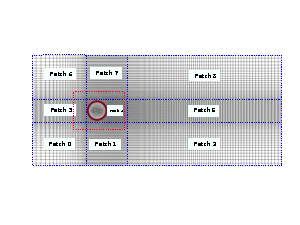
\includegraphics[scale=3.0,trim=0cm 1cm 0cm 0.8cm, clip=true]{Imagens/Cap6/aerofolio_malhaArlequin.pdf}}\\
	\subfloat[Discretização da malha local\label{fig:aerofolio_detalheLocal}]{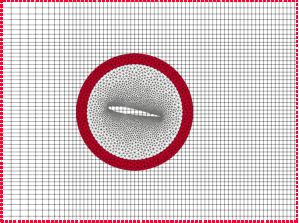
\includegraphics[trim=0 0 0 0,clip=true,scale=1.5]{Imagens/Cap6/aerofolio_detalheLocal.pdf}}
	\label{fig:aerofolio_malhaArlequin_detalheLocal}
	\legend{Fonte: Elaborada pela autora}
\end{figure}

A malha global isogeométrica foi obtida através da utilização de 9 $patches$, que totalizaram 15561 pontos de controle e 14025 células. A discretização em cada \textit{patch} pode ser visualizada na \autoref{tab:aerofolio_discretização_patches}. A malha local por sua vez é composta por 5214 elementos triangulares quadráticos e 10670 nós. 

\begin{table}[h]
	\caption{Aerofólio: Número de pontos de controle por \textit{patch}}
	\label{tab:aerofolio_discretização_patches}
	\centering
	\begin{minipage}{0.49\textwidth}
		\centering
		\begin{tabular}{cccc} 
			\toprule
			\textit{Patch} & $\xsi$ & $\eta$\\ 
			\midrule \midrule
			0 & 27 & 27\\
			\midrule
			1 & 62 & 27\\
			\midrule
			2 & 82 & 27\\
			\midrule
			3 & 27 & 37\\
			\midrule
			4 & 62 & 37\\
			\midrule
			5 & 82 & 37\\ 
			\midrule
			6 & 27 & 27\\ 
			\midrule
			7 & 62 & 27\\ 
			\midrule
			8 & 82 & 27\\ 
			\bottomrule
		\end{tabular}
	\end{minipage}%
	\fonte{Elaborada pelo autor.}%
\end{table}

Na Figura \ref{fig:aerofolio_detalheLocal} pode observar em vermelho os elementos que fazem parte da zona de colagem. A espessura da zona de colagem foi definida como $0,2$, totalizando 628 elementos triangulares quadráticos e 1428 nós nessa região. A constante do operador de acoplamento $L^{2}$ foi definida como $k_{0} = 10$. 

Nesse problema observa-se o surgimento de uma esteira de vórtices a jusante do aerofólio, que resulta em um número de Strouhal ($\Strouhal$) equivalente a 0,877. Esse valor encontra-se em concordância com o obtido por \citeonline{MittalT:1994} de 0,862. 

Nas Figura \ref{fig:aerofolio_CD} e Figura \ref{fig:aerofolio_CL} apresentam-se os resultados de coeficiente de arrasto e sustentação obtidos para as análises realizadas. Pode-se observar que os resultados obtidos com o modelo baseado no método Arlequin estabilizados estão de acordo com os obtidos para o modelo usando monomodelo.

\begin{figure}[!htbp]
	\caption{Aerofólio: Coeficiente de Arrasto}
	\centering 
	{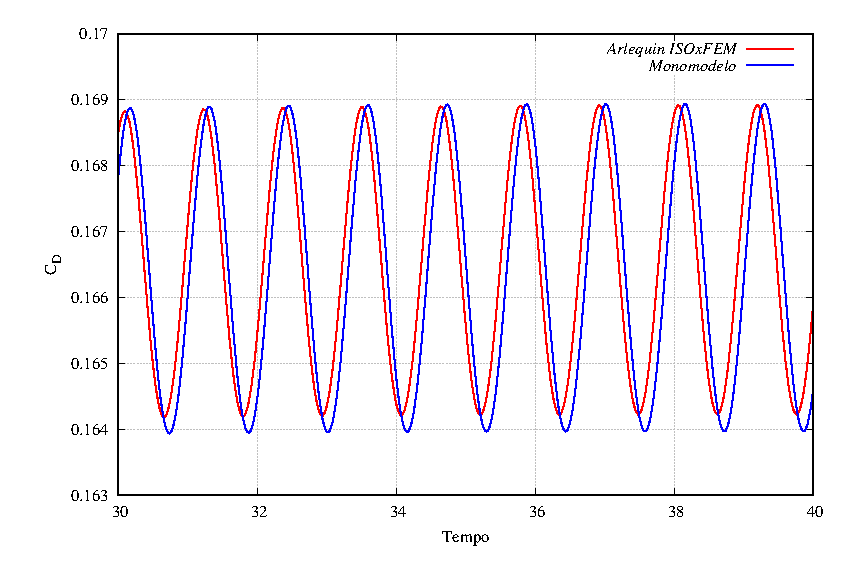
\includegraphics[scale=0.8,trim=0cm 0cm 0cm 0cm, clip=true]{Imagens/Cap6/aerofolio_CD.eps}}	
	\label{fig:aerofolio_CD}
	\legend{Fonte: Elaborada pela autora}
\end{figure}

\begin{figure}[!htbp]
	\caption{Aerofólio: Coeficiente de Arrasto}
	\centering 
	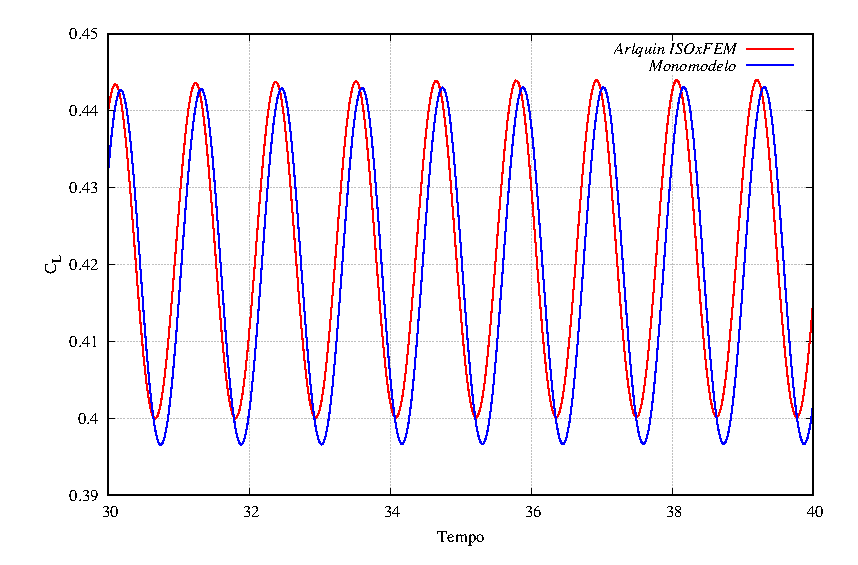
\includegraphics[scale=0.8,trim=0cm 0cm 0cm 0cm, clip=true]{Imagens/Cap6/aerofolio_CL.eps}	
	\label{fig:aerofolio_CL}
	\legend{Fonte: Elaborada pela autora}
\end{figure}

Nas Figura \ref{fig:aerofolio_velocidade} e Figura \ref{fig:aerofolio_pressao} estão apresentados os campos de velocidade e pressão respectivamente para um período de um ciclo das curvas referentes aos coeficientes de arrasto e sustentação. 

\begin{figure}[!htbp]
	\caption{Aerofólio: Campo de velocidade}
	\centering
	\subfloat[$nT$]{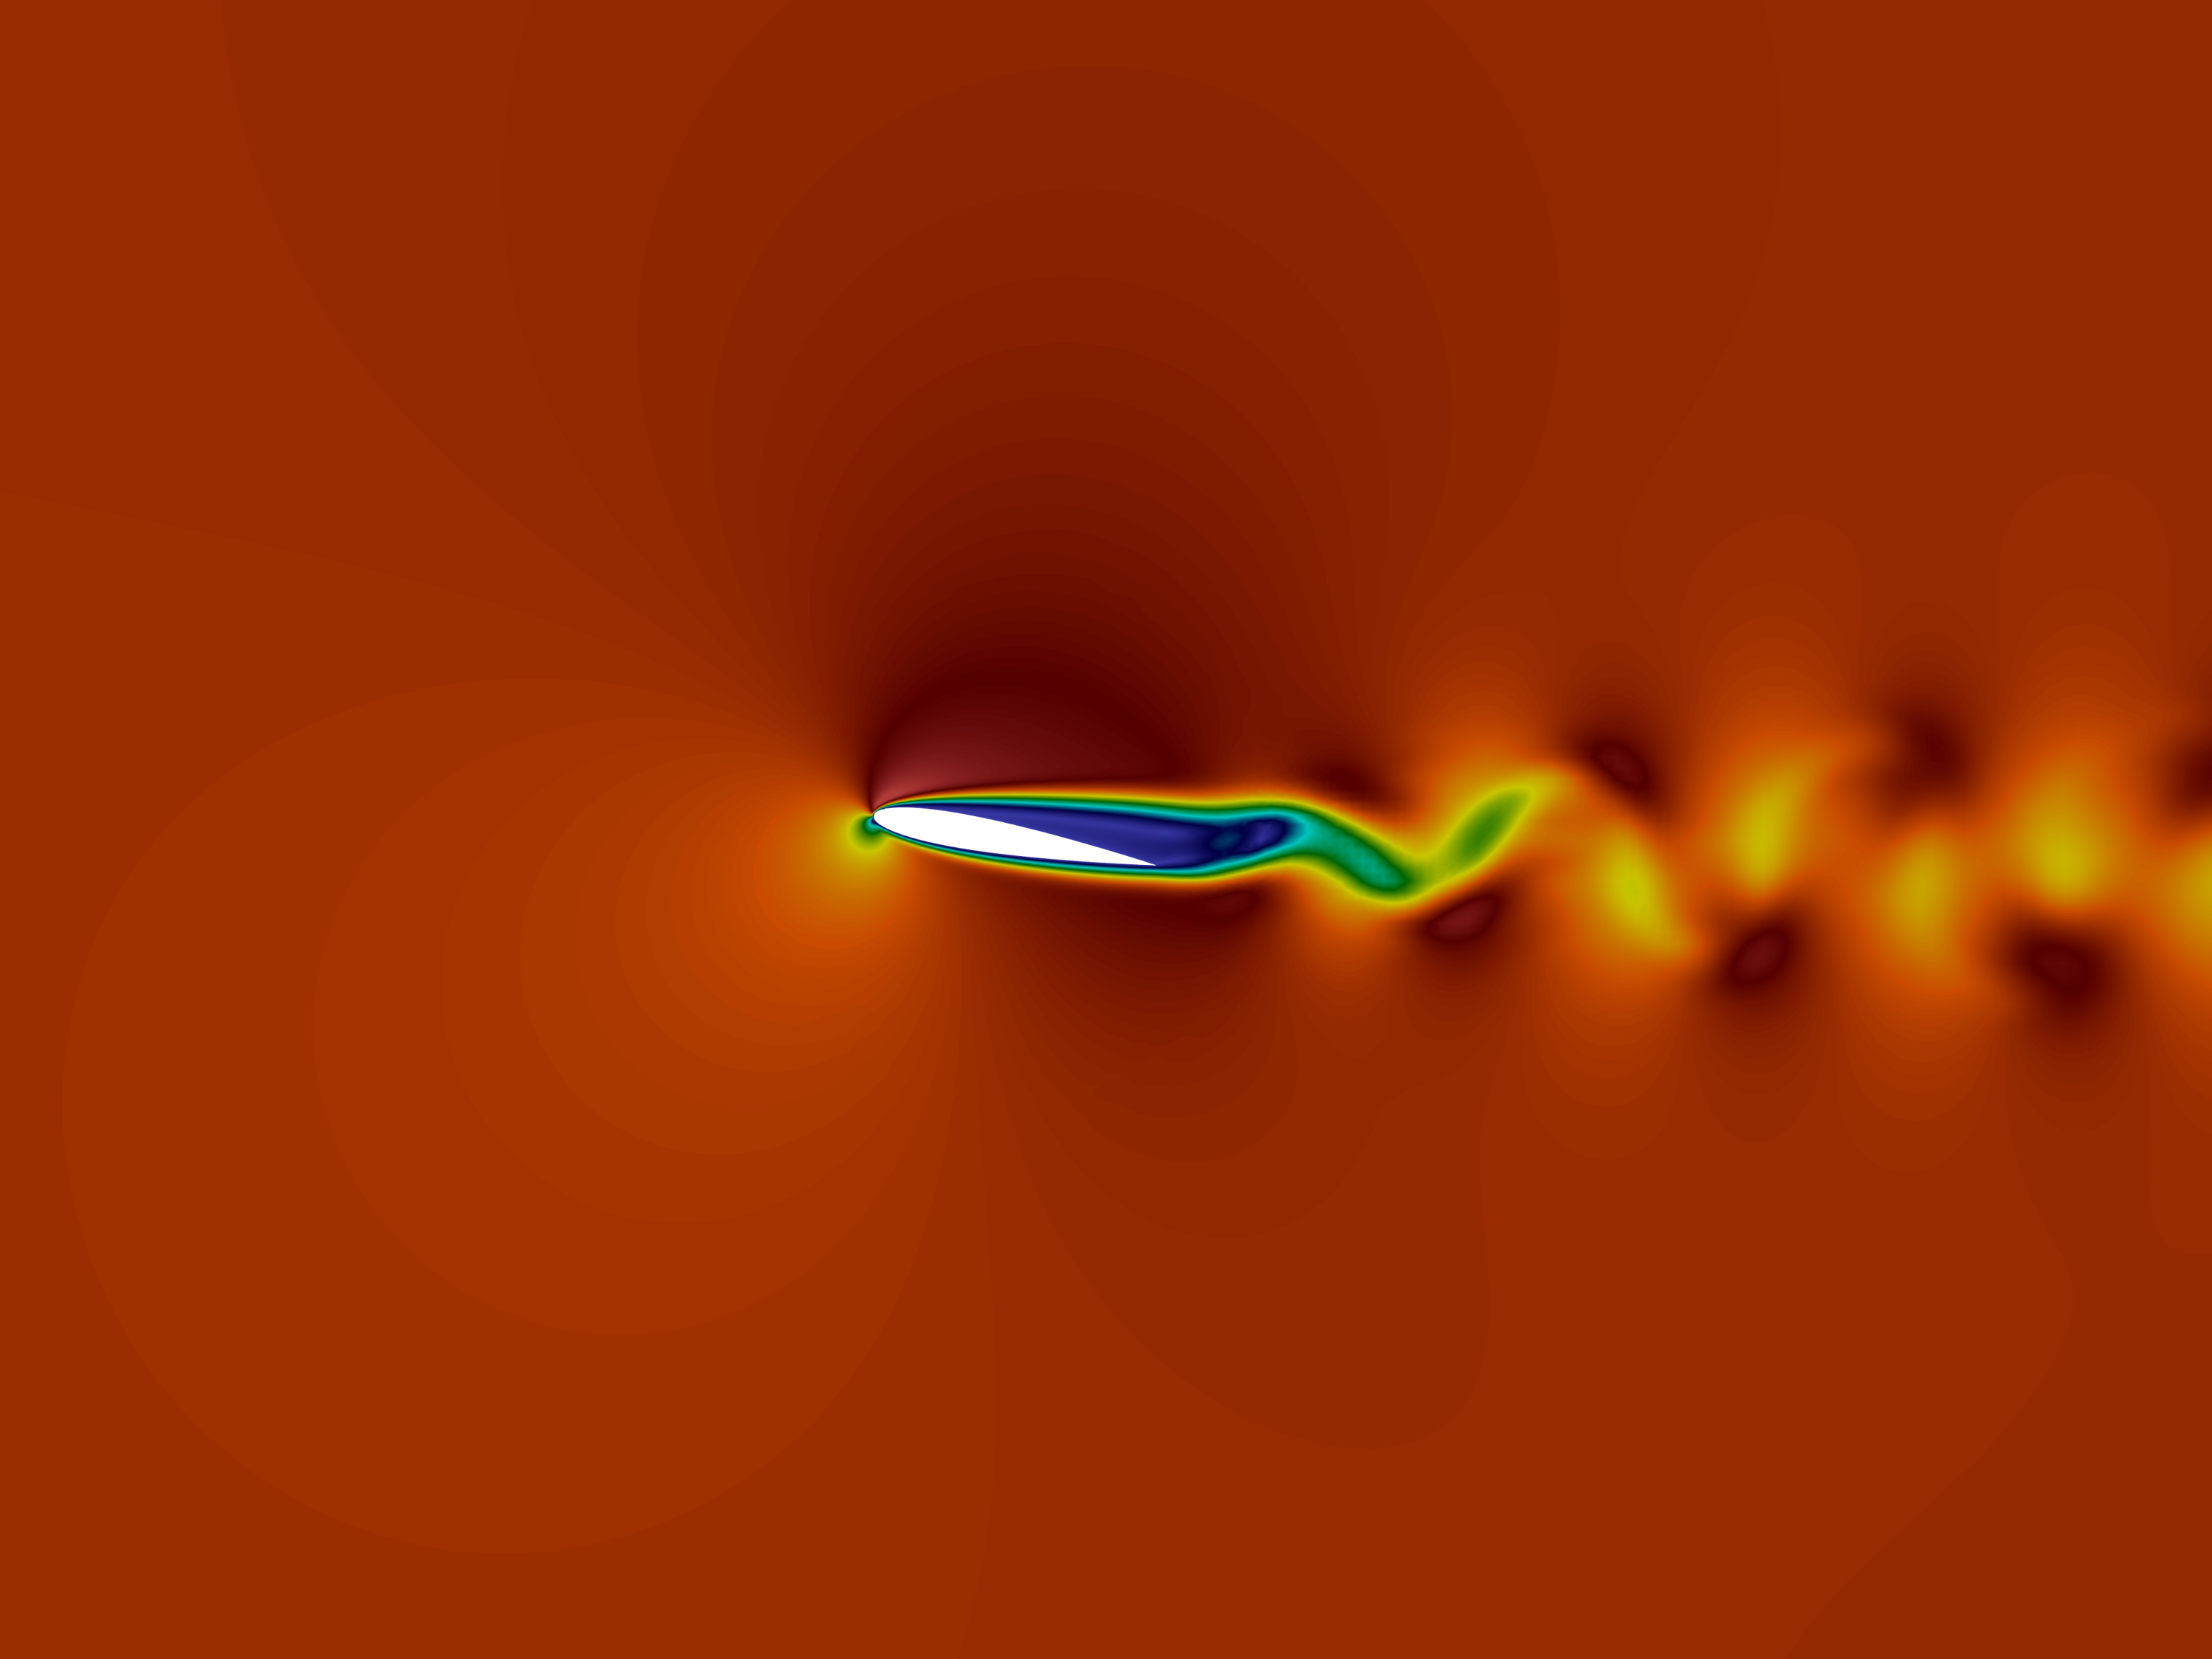
\includegraphics[scale=0.13,trim=0cm 0cm 0cm 0cm, clip=true]{Imagens/Cap6/aerofolio_velTn.pdf}} \ \
	\subfloat[$nT + nT/4$]{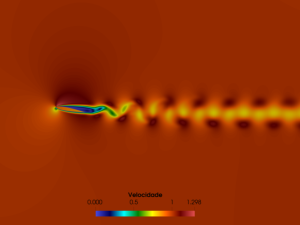
\includegraphics[trim=0 0 0 0,clip=true,scale=0.13]{Imagens/Cap6/aerofolio_velTn4.pdf}} \\
	\subfloat[$nT + nT/2$]{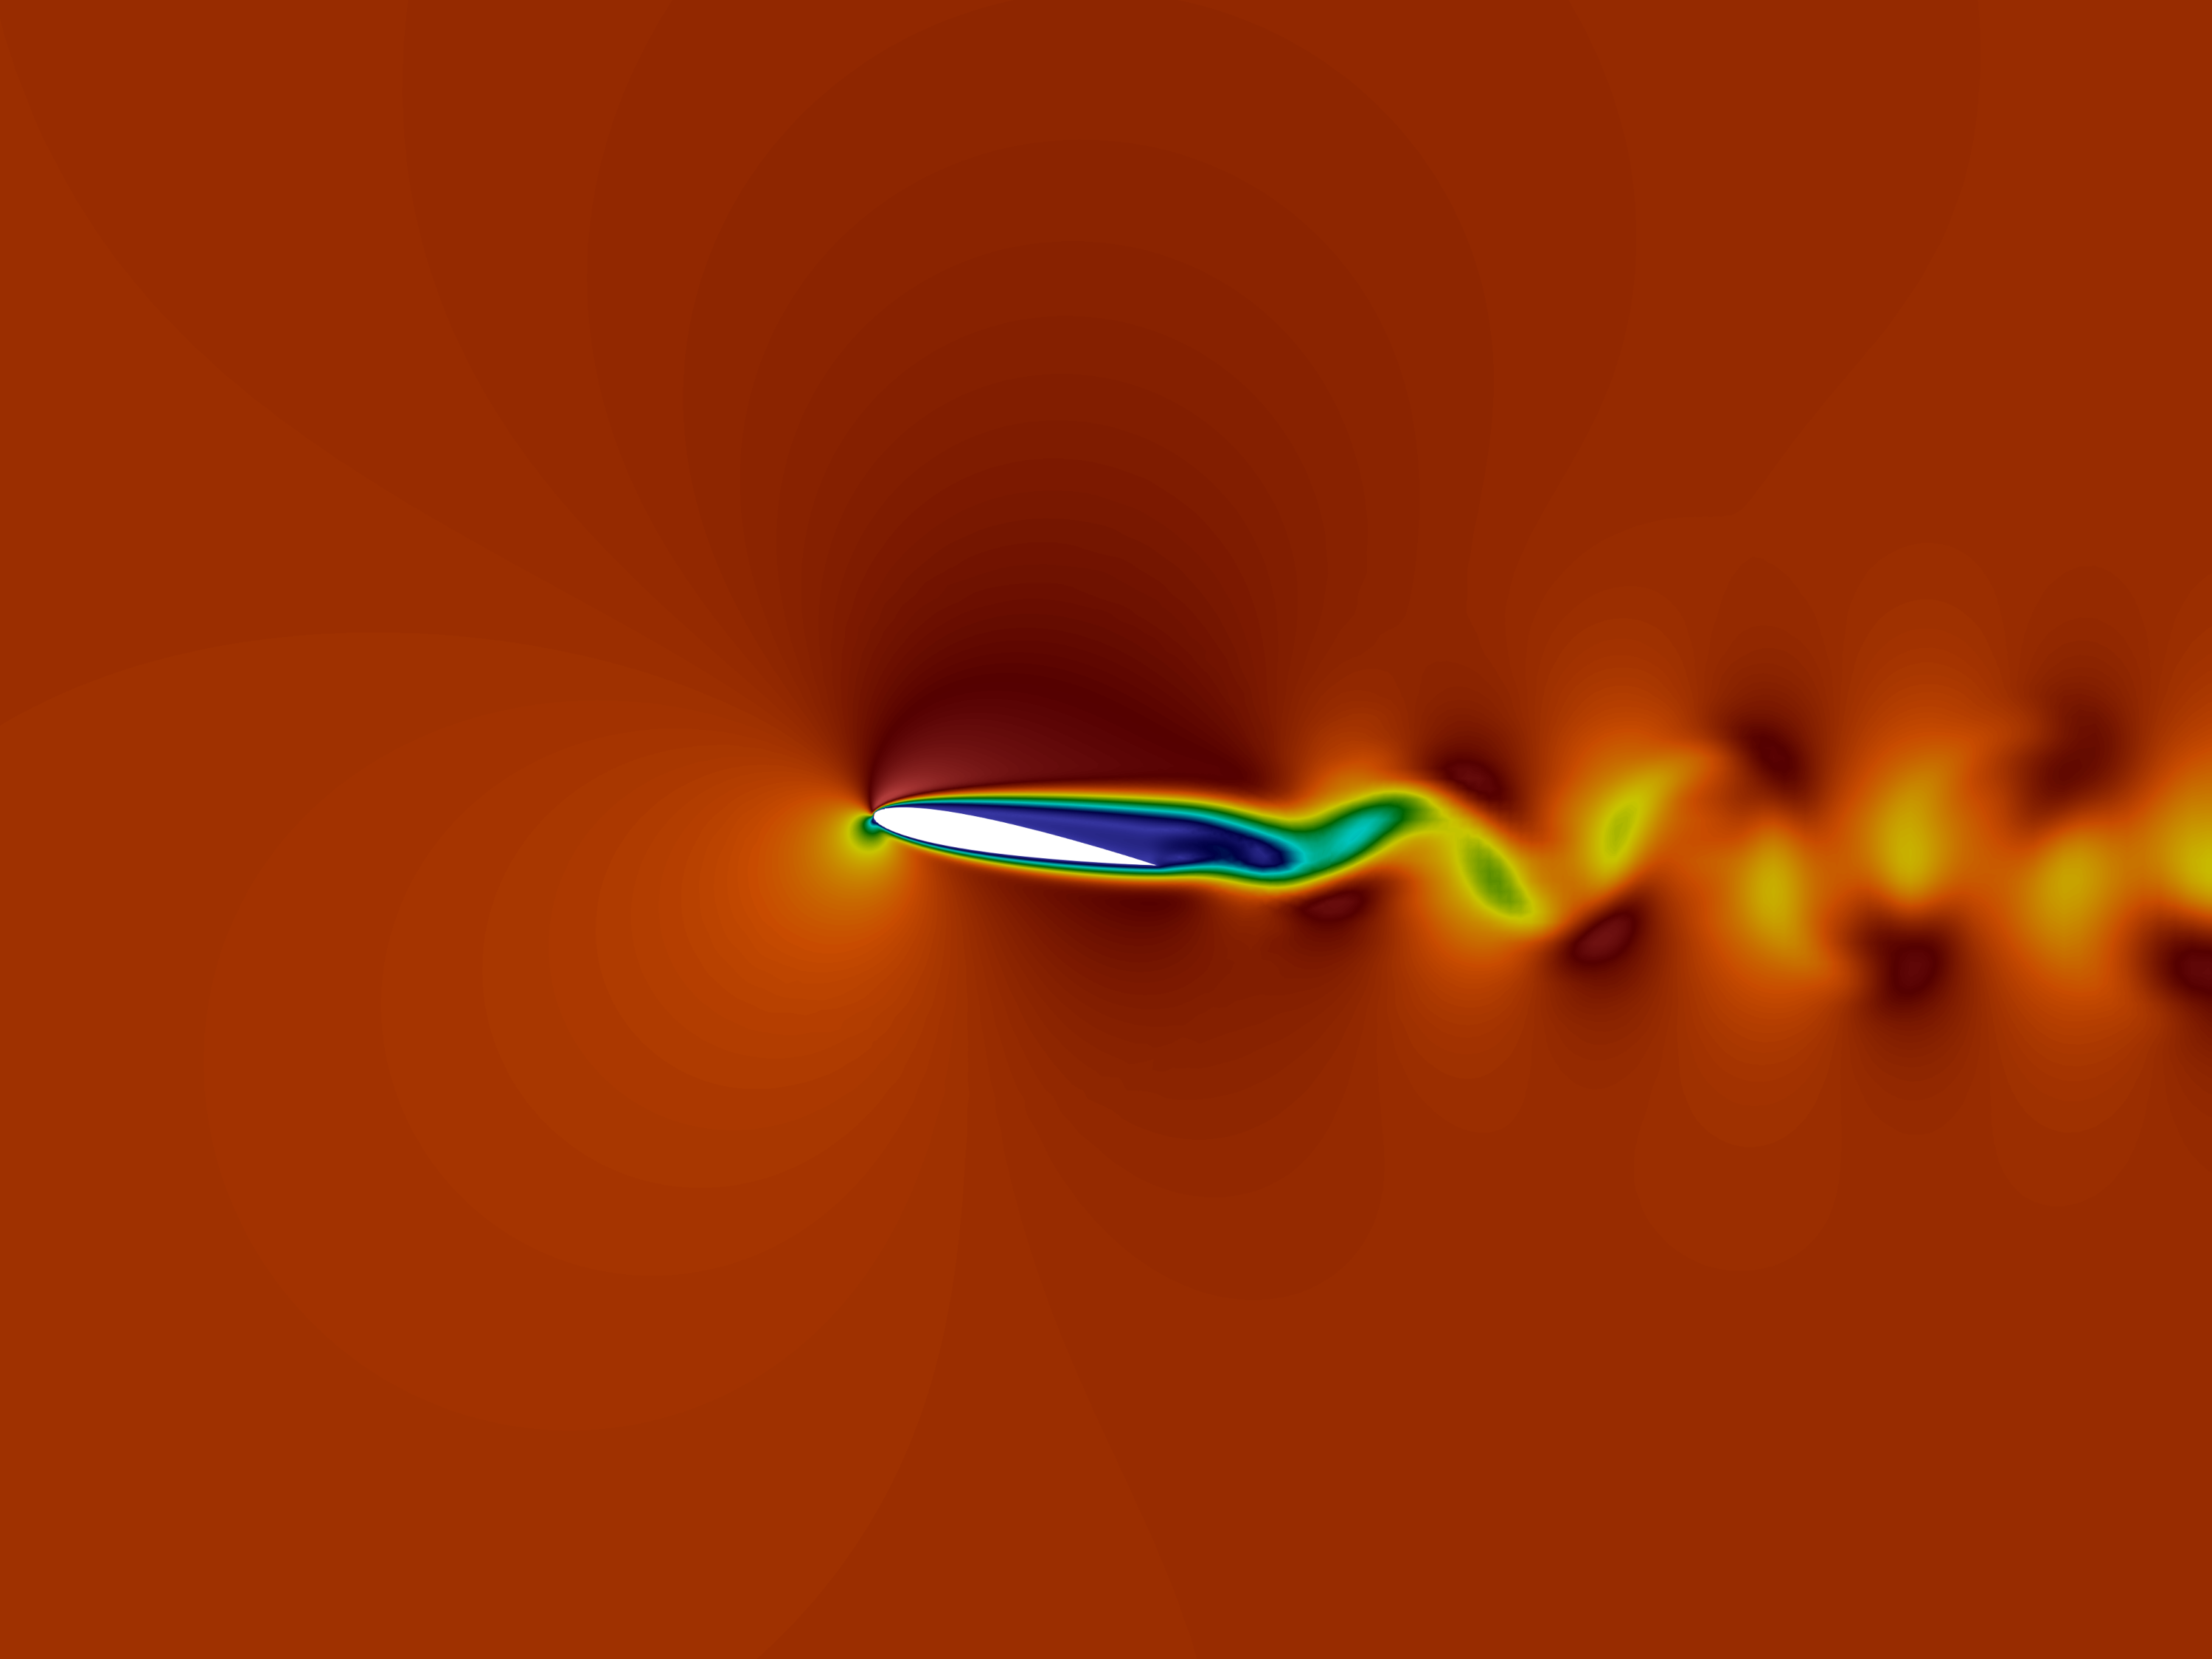
\includegraphics[scale=0.13,trim=0cm 0cm 0cm 0cm, clip=true]{Imagens/Cap6/aerofolio_velTn2.pdf}} \ \
	\subfloat[$nT + n3T/4$]{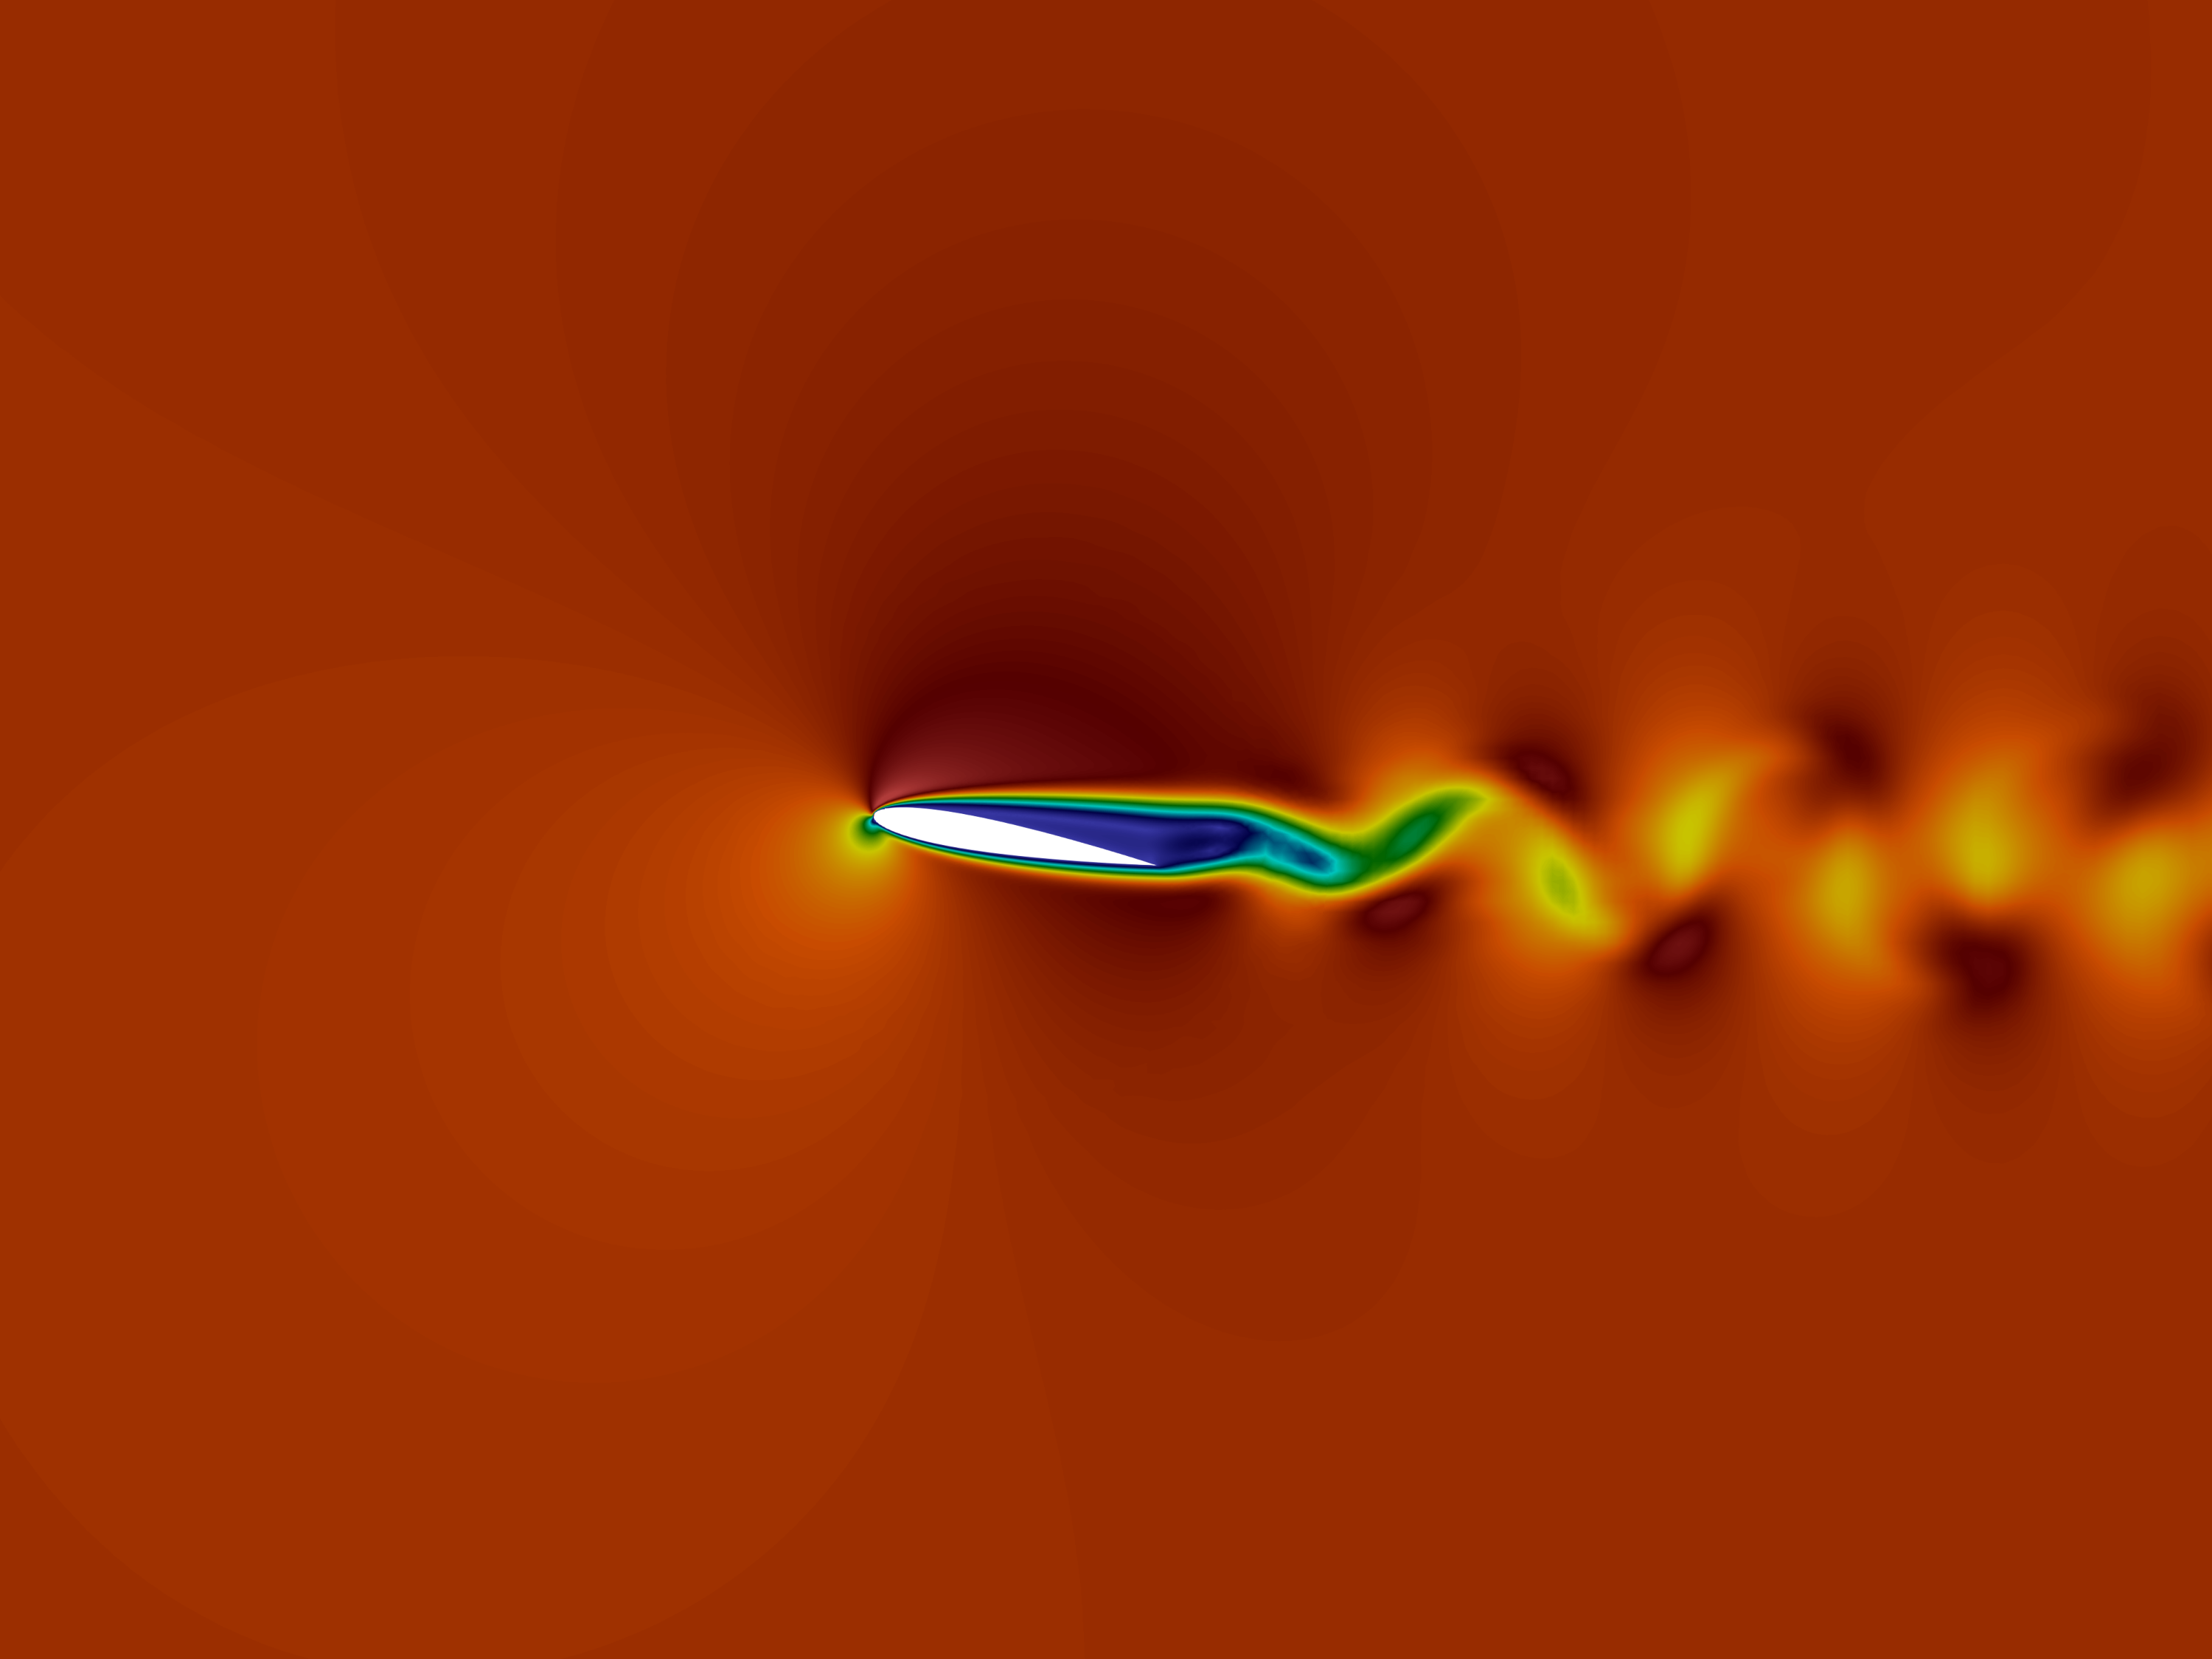
\includegraphics[trim=0 0 0 0,clip=true,scale=0.13]{Imagens/Cap6/aerofolio_velTn34.pdf}} \\
	{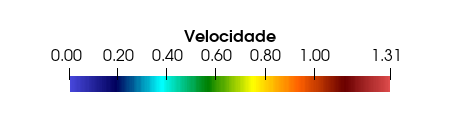
\includegraphics[trim=0 0.2cm 0 0,clip=true,scale=0.4]{Imagens/Cap6/aerofolio_velLegenda.png}}
	\label{fig:aerofolio_velocidade}
	\legend{Fonte: Elaborada pela autora}
\end{figure}

\begin{figure}[!htbp]
	\caption{Aerofólio: Campo de pressão}
	\centering
	\subfloat[$nT$]{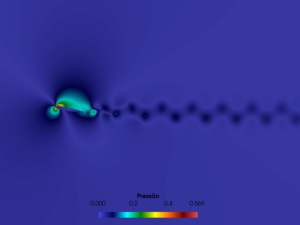
\includegraphics[scale=0.13,trim=0cm 0cm 0cm 0cm, clip=true]{Imagens/Cap6/aerofolio_pressTn.pdf}} \ \
	\subfloat[$nT + nT/4$]{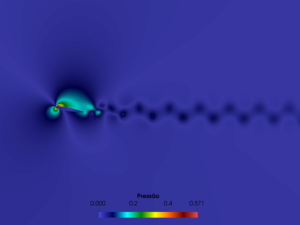
\includegraphics[trim=0 0 0 0,clip=true,scale=0.13]{Imagens/Cap6/aerofolio_pressTn4.pdf}} \\
	\subfloat[$nT + nT/2 $]{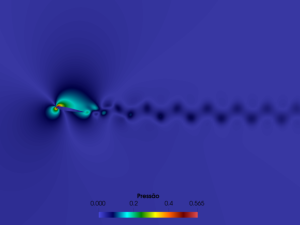
\includegraphics[scale=0.13,trim=0cm 0cm 0cm 0cm, clip=true]{Imagens/Cap6/aerofolio_pressTn2.pdf}} \ \
	\subfloat[$nT + n3T/4$]{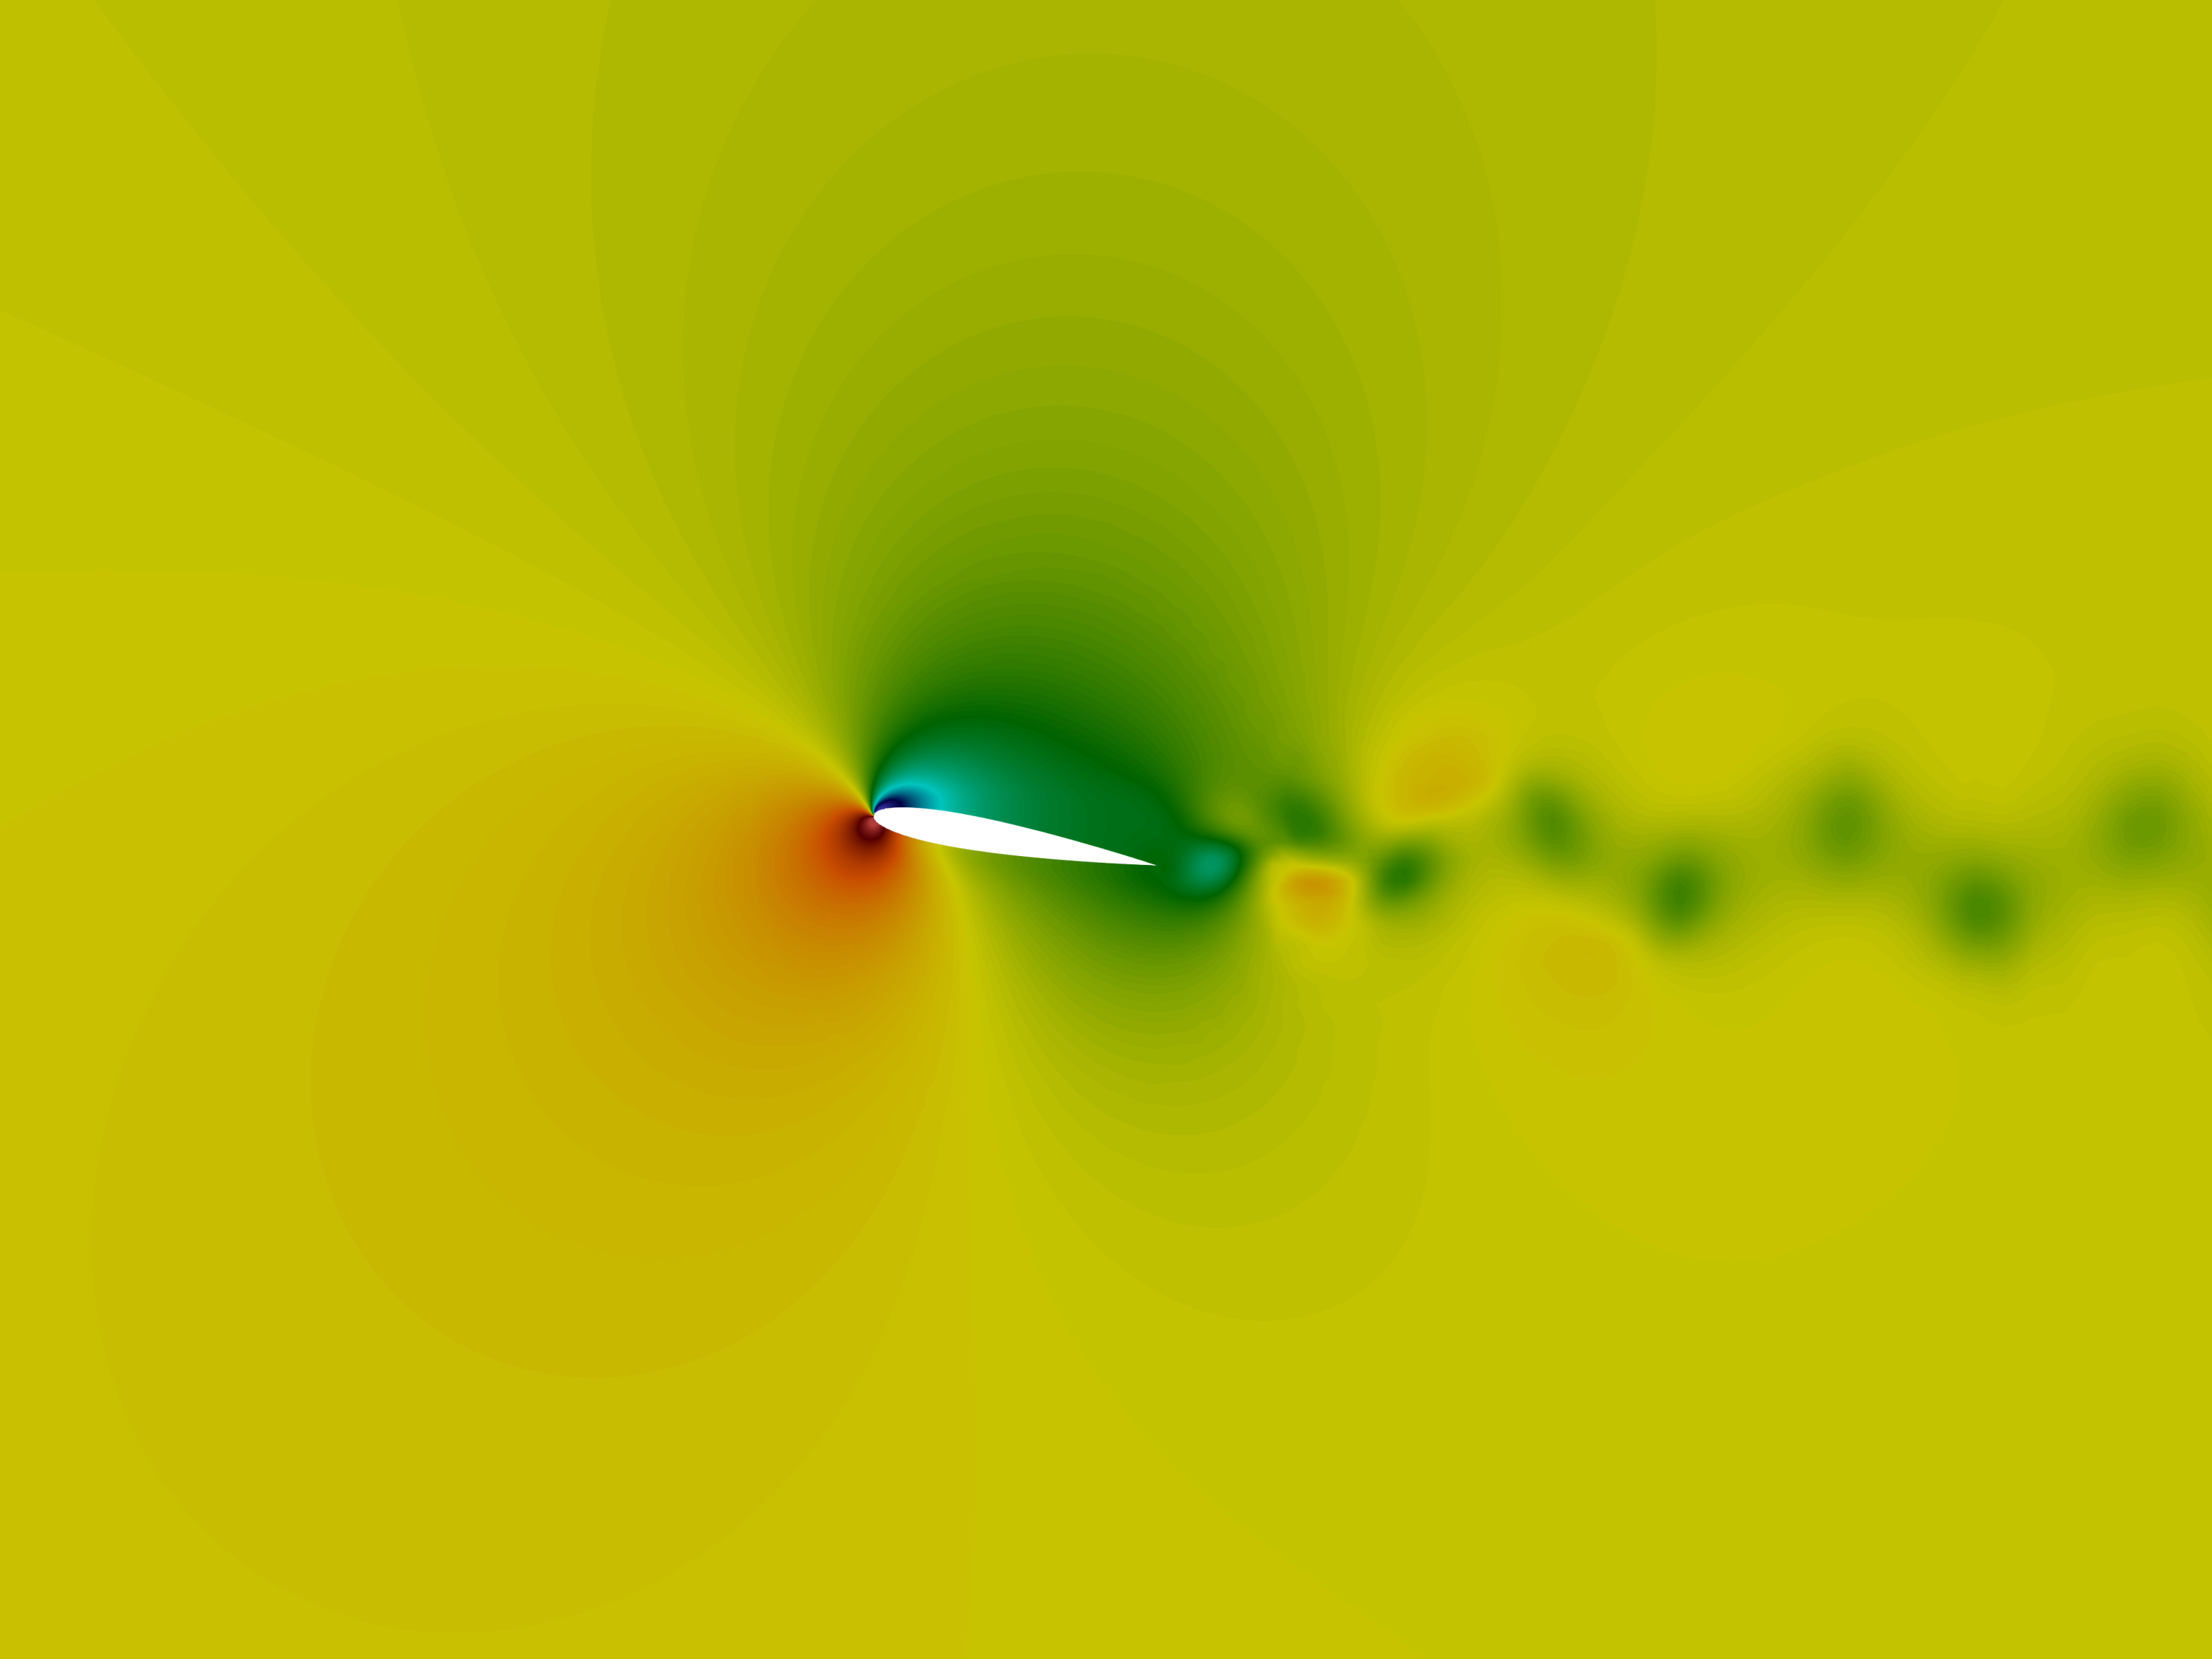
\includegraphics[trim=0 0 0 0,clip=true,scale=0.13]{Imagens/Cap6/aerofolio_pressTn34.pdf}}\\
	{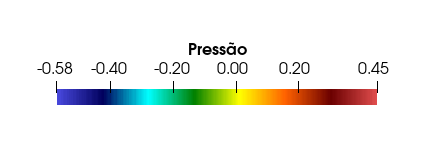
\includegraphics[trim=0 0.8cm 0 0cm,clip=true,scale=0.4]{Imagens/Cap6/aerofolio_pressLegenda.png}}
	\legend{Fonte: Elaborada pela autora}
	\label{fig:aerofolio_pressao}
\end{figure}

\subsection{Aerofólio com movimento de arfagem prescrito}

Para a validação computacional da técnica Arlequin estabilizada em domínios móveis  utilizou-se um problema envolvendo um aerofólio NACA 0012, semelhante ao apresentado na \autoref{capitulo:Cap6:Exemplos:NACA0012}, aplicando-se, entretanto, um movimento de arfagem ao mesmo. O aerofólio apresenta variação do ângulo de ataque em $20^{\circ}$, iniciando o movimento em $10^{\circ}$ e finalizando-o em $30^{\circ}$. 

Para descrever-se tal movimento aplica-se, tendo como centro a corda média do aerofólio, o movimento de rotação de corpo rígido através da seguinte relação:

\begin{align}
	\theta = \frac{\theta_{max}+\theta_{min}}{2} - \frac{\theta_{max}-\theta_{min}}{2}\cos{\omega_{f}t} ,
\end{align}

\noindent com $\omega_{f} = 2\pi f_{o}$, sendo $f_{o}$ a frequência de oscilação, adotada nesse estudo como 1.0, $\theta_{max} = 30^{\circ}$ e $\theta_{min} = 10^{\circ}$.

As dimensões da geometria do domínio computacional são alteradas (ver \autoref{fig:aerofolioMov_geometria}) para capturar os efeitos dos desprendimentos de vórtices, que para esse problema, se desprendem em uma faixa mais ampla. Os demais parâmetros de análise foram mantidos iguais aos apresentados no exemplo da \autoref{capitulo:Cap6:Exemplos:NACA0012}. 

\begin{figure}[!htbp]
	\caption{Aerofólio Mov.: Geometria}
	\centering 
	{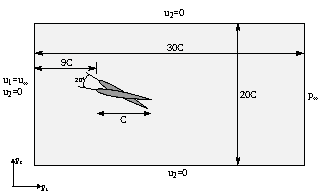
\includegraphics[scale=2.0,trim=0cm 0cm 0cm 0cm, clip=true]{Imagens/Cap6/aerofolioMov_geometria.pdf}}	
	\label{fig:aerofolioMov_geometria}
	\legend{Fonte: Elaborada pela autora}
\end{figure}

Novamente são analisadas 2 discretizações: 1. Monomodelo; 2. Combinação de duas malhas através do método Arlequin estabilizado.
O monomodelo consiste em uma malha com 12438 elementos triangulares quadráticos e 25188 elementos. As malhas global e local do método Arlequin mantiveram-se com a mesma discretização do problema da \autoref{capitulo:Cap6:Exemplos:NACA0012}, incluindo a quantidade de elementos na zona de colagem.

É importante ressaltar que para a simulação desse exemplo, utilizou-se como campo inicial de velocidade e pressão, valores obtidos em uma solução de longo termo do aerofólio na condição de repouso.

A variação dos coeficientes de arrasto e sustentação ao longo do tempo são apresentados nas \autoref{fig:aerofolioMov_CD} e \autoref{fig:aerofolioMov_CL}. Nota-se nas imagens que o monomodelo e o modelo Arlequin estão consistentes em suas respostas. Soluções semelhantes podem ser observados no trabalho de \citeonline{Fernandes:2020}.

\begin{figure}[!htbp]
	\caption{Aerofólio Mov.: Coeficiente de Arrasto}
	\centering 
	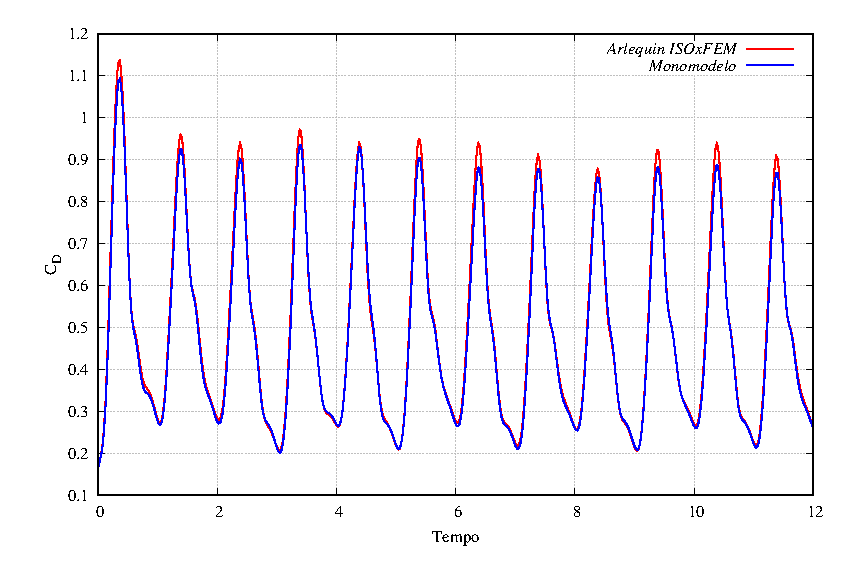
\includegraphics[scale=0.8,trim=0cm 0cm 0cm 0cm, clip=true]{Imagens/Cap6/aerofolioMov_CD.eps}	
	\label{fig:aerofolioMov_CD}
	\legend{Fonte: Elaborada pela autora}
\end{figure}

\begin{figure}[!htbp]
	\caption{Aerofólio Mov.: Coeficiente de Sustentação}
	\centering 
	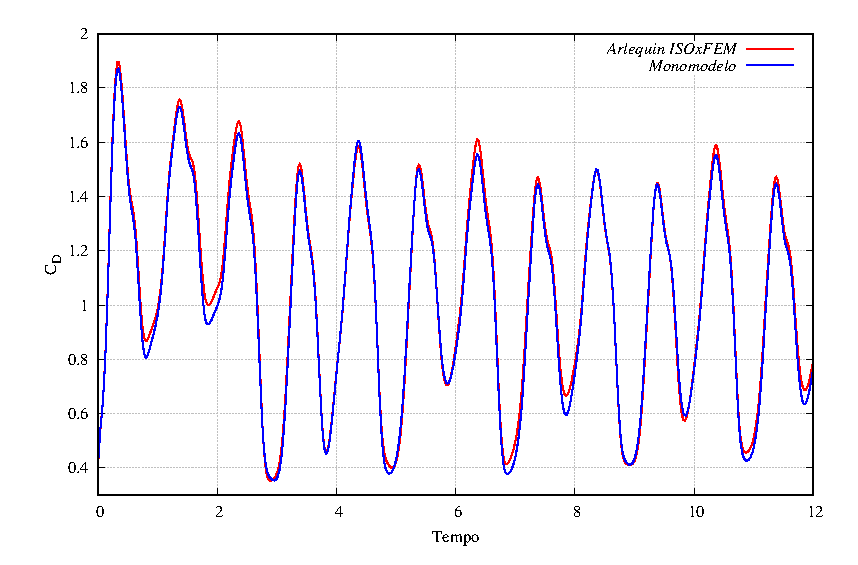
\includegraphics[scale=0.8,trim=0cm 0cm 0cm 0cm, clip=true]{Imagens/Cap6/aerofolioMov_CL.eps}	
	\label{fig:aerofolioMov_CL}
	\legend{Fonte: Elaborada pela autora}
\end{figure}

Na Figura \ref{fig:aerofolioMov_velocidade} e Figura \ref{fig:aerofolioMov_pressao} são apresentados os campos de velocidade e pressão em alguns instantes para um ciclo do movimento oscilatório prescrito.

\begin{figure}[!htbp]
	\caption{Aerofólio Mov.: Campos de velocidade}
	\centering
	\subfloat[$t = 8,0 $]{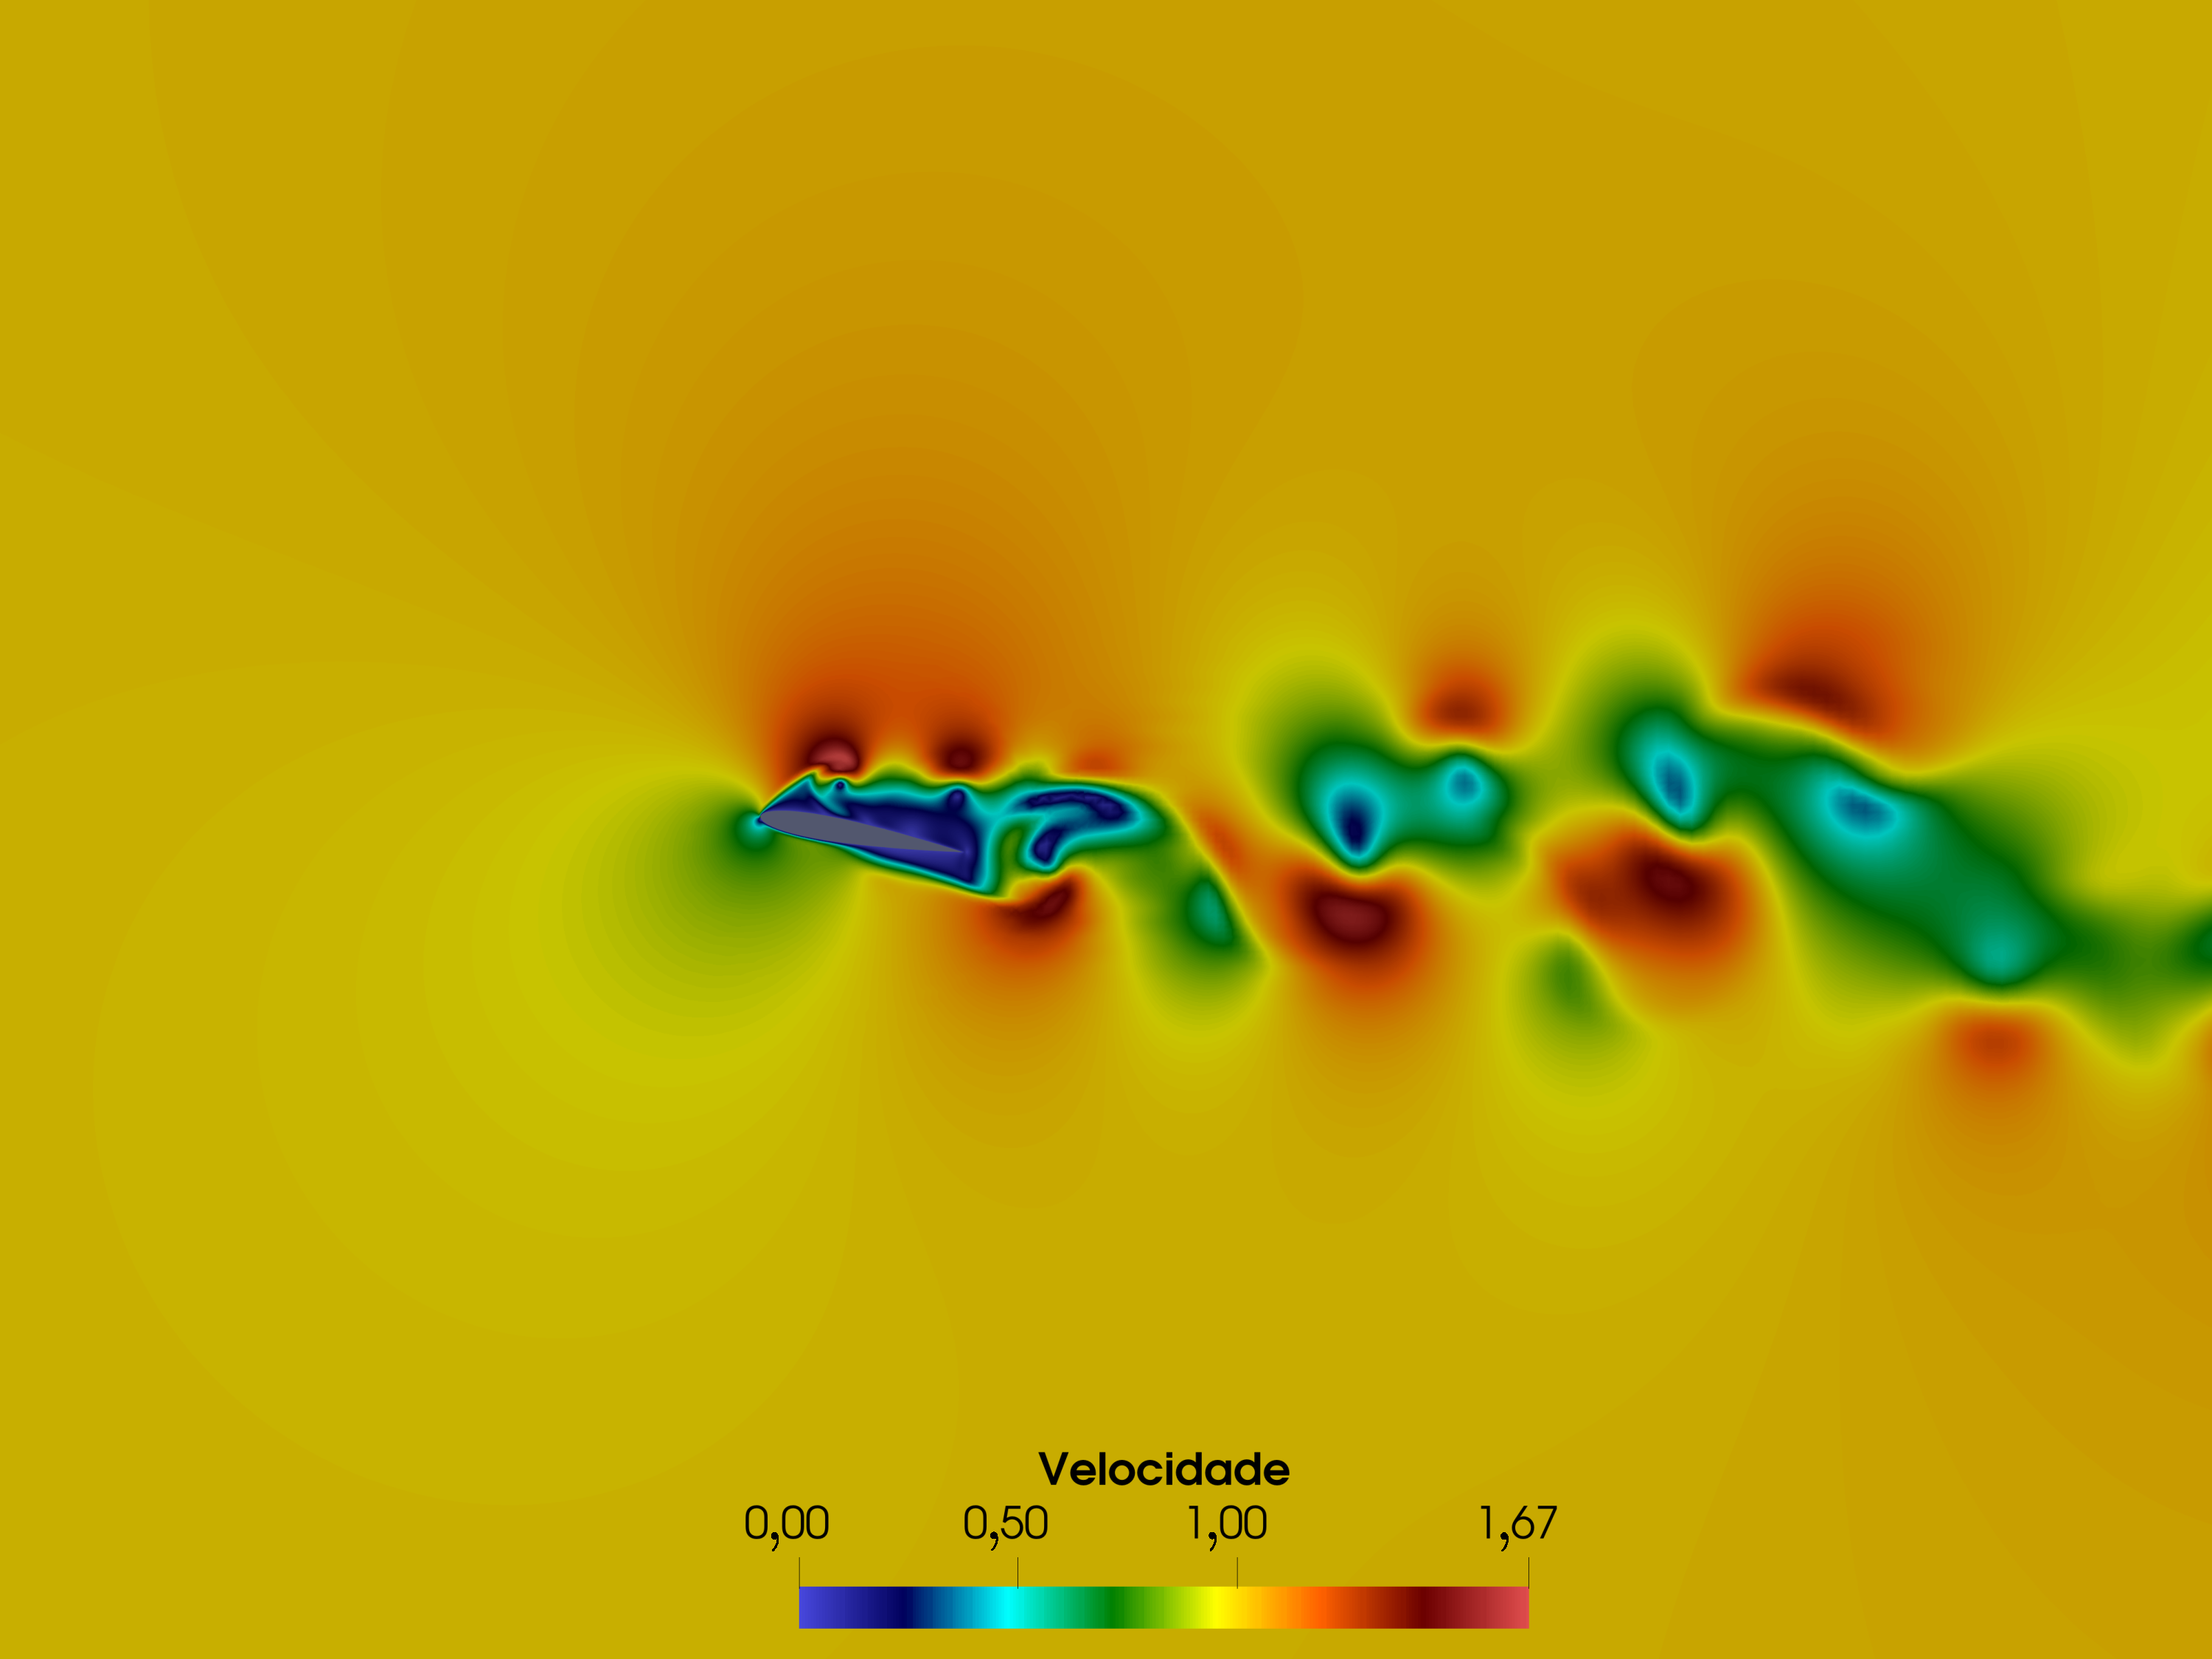
\includegraphics[scale=0.13,trim=0cm 0cm 0cm 0cm, clip=true]{Imagens/Cap6/aerofolioMov_vel400.pdf}} \
	\subfloat[$t = 8,3 $]{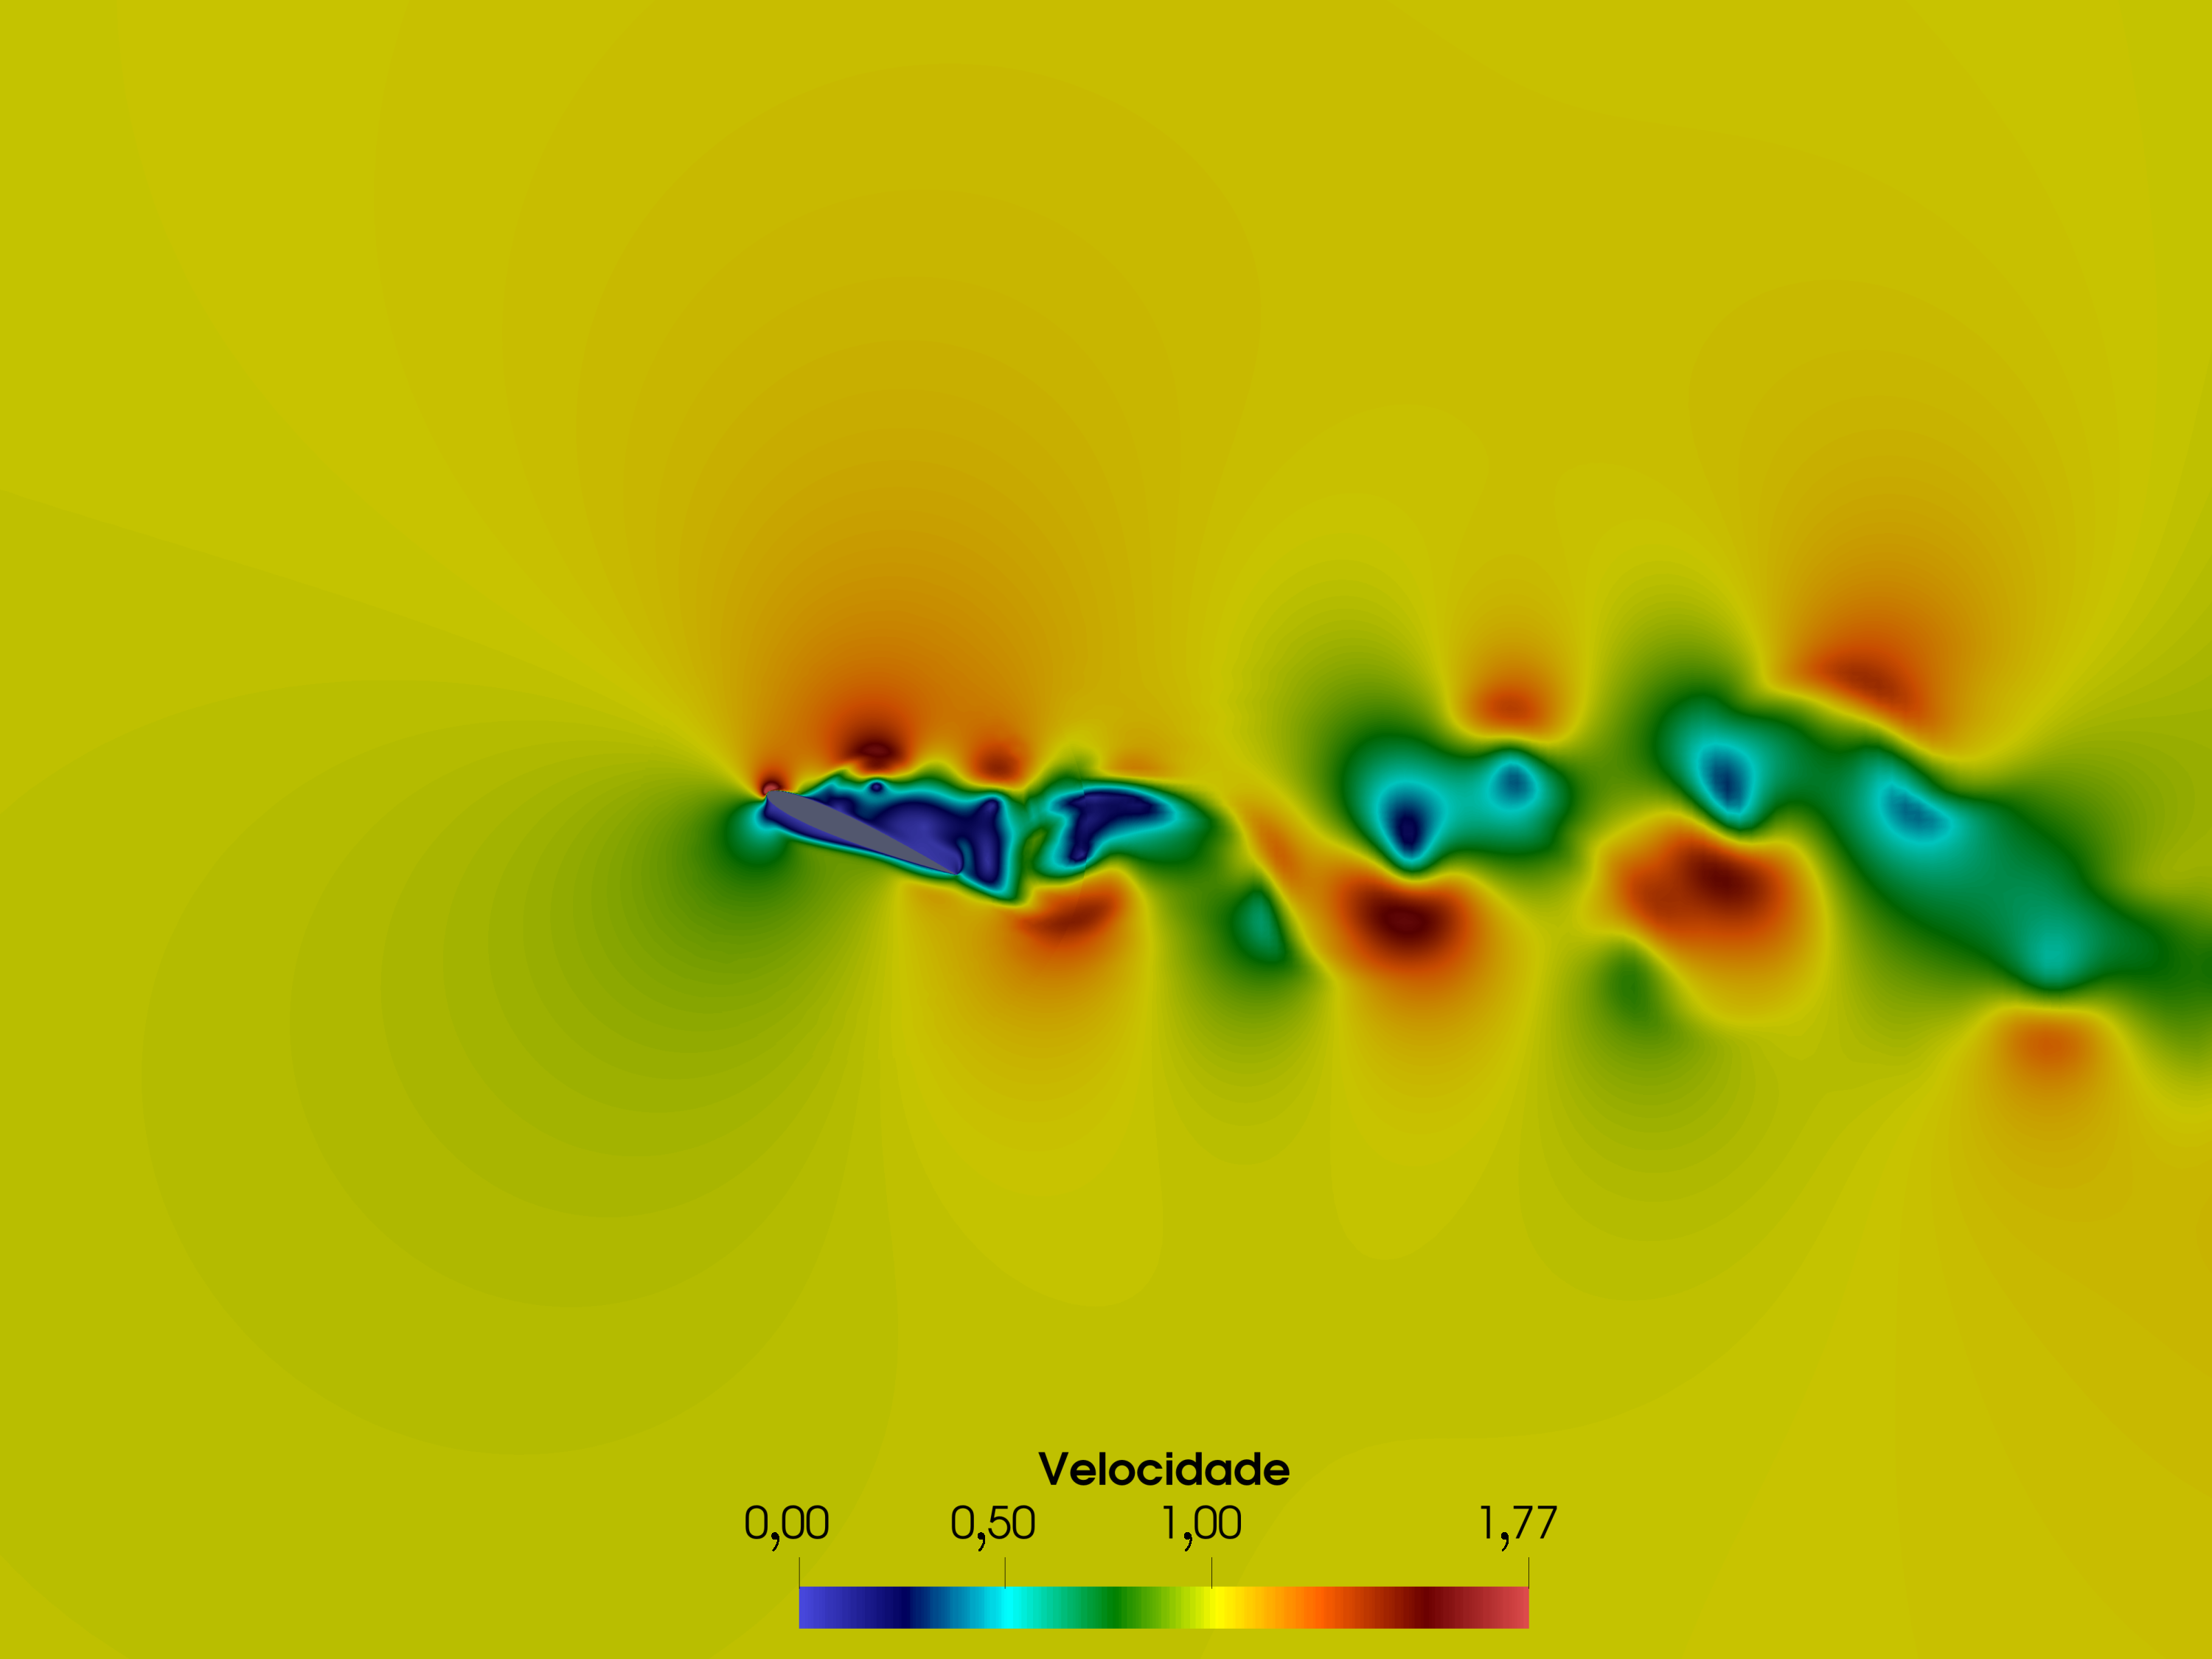
\includegraphics[trim=0 0 0 0,clip=true,scale=0.13]{Imagens/Cap6/aerofolioMov_vel415.pdf}}\\
	\subfloat[$t = 8,5 $]{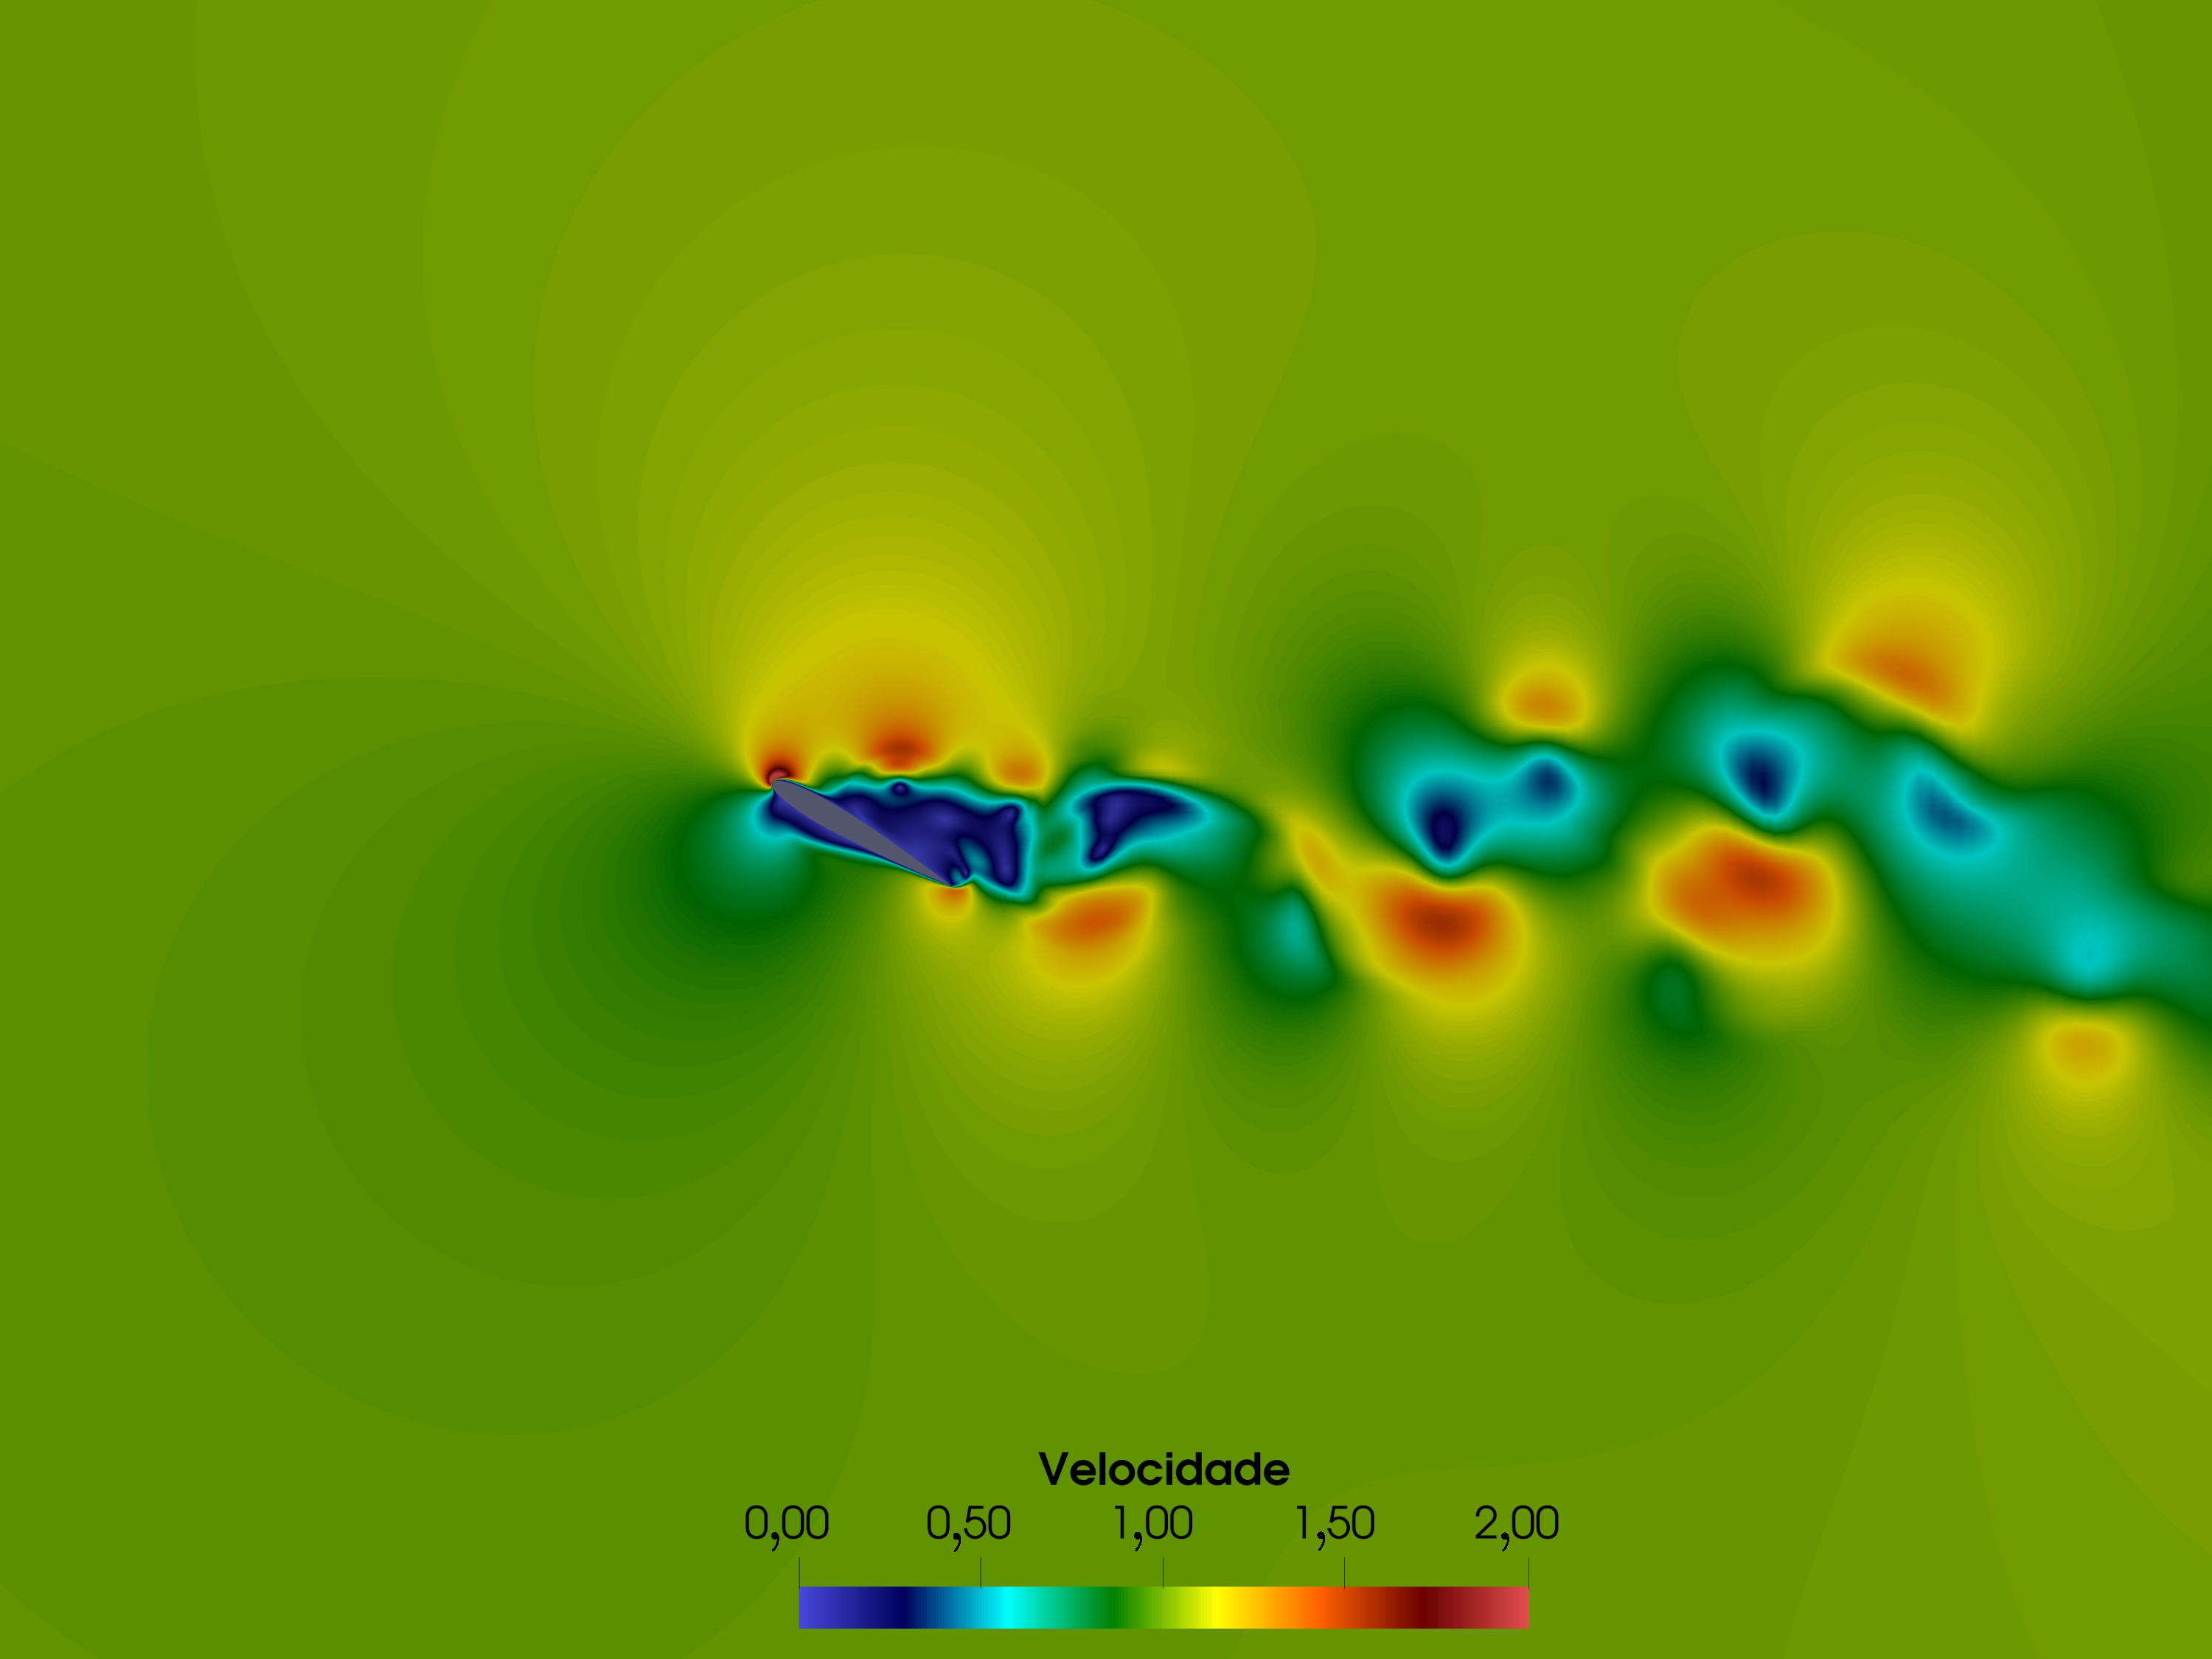
\includegraphics[scale=0.13,trim=0cm 0cm 0cm 0cm, clip=true]{Imagens/Cap6/aerofolioMov_vel425.pdf}} \
	\subfloat[$t = 8,8 $]{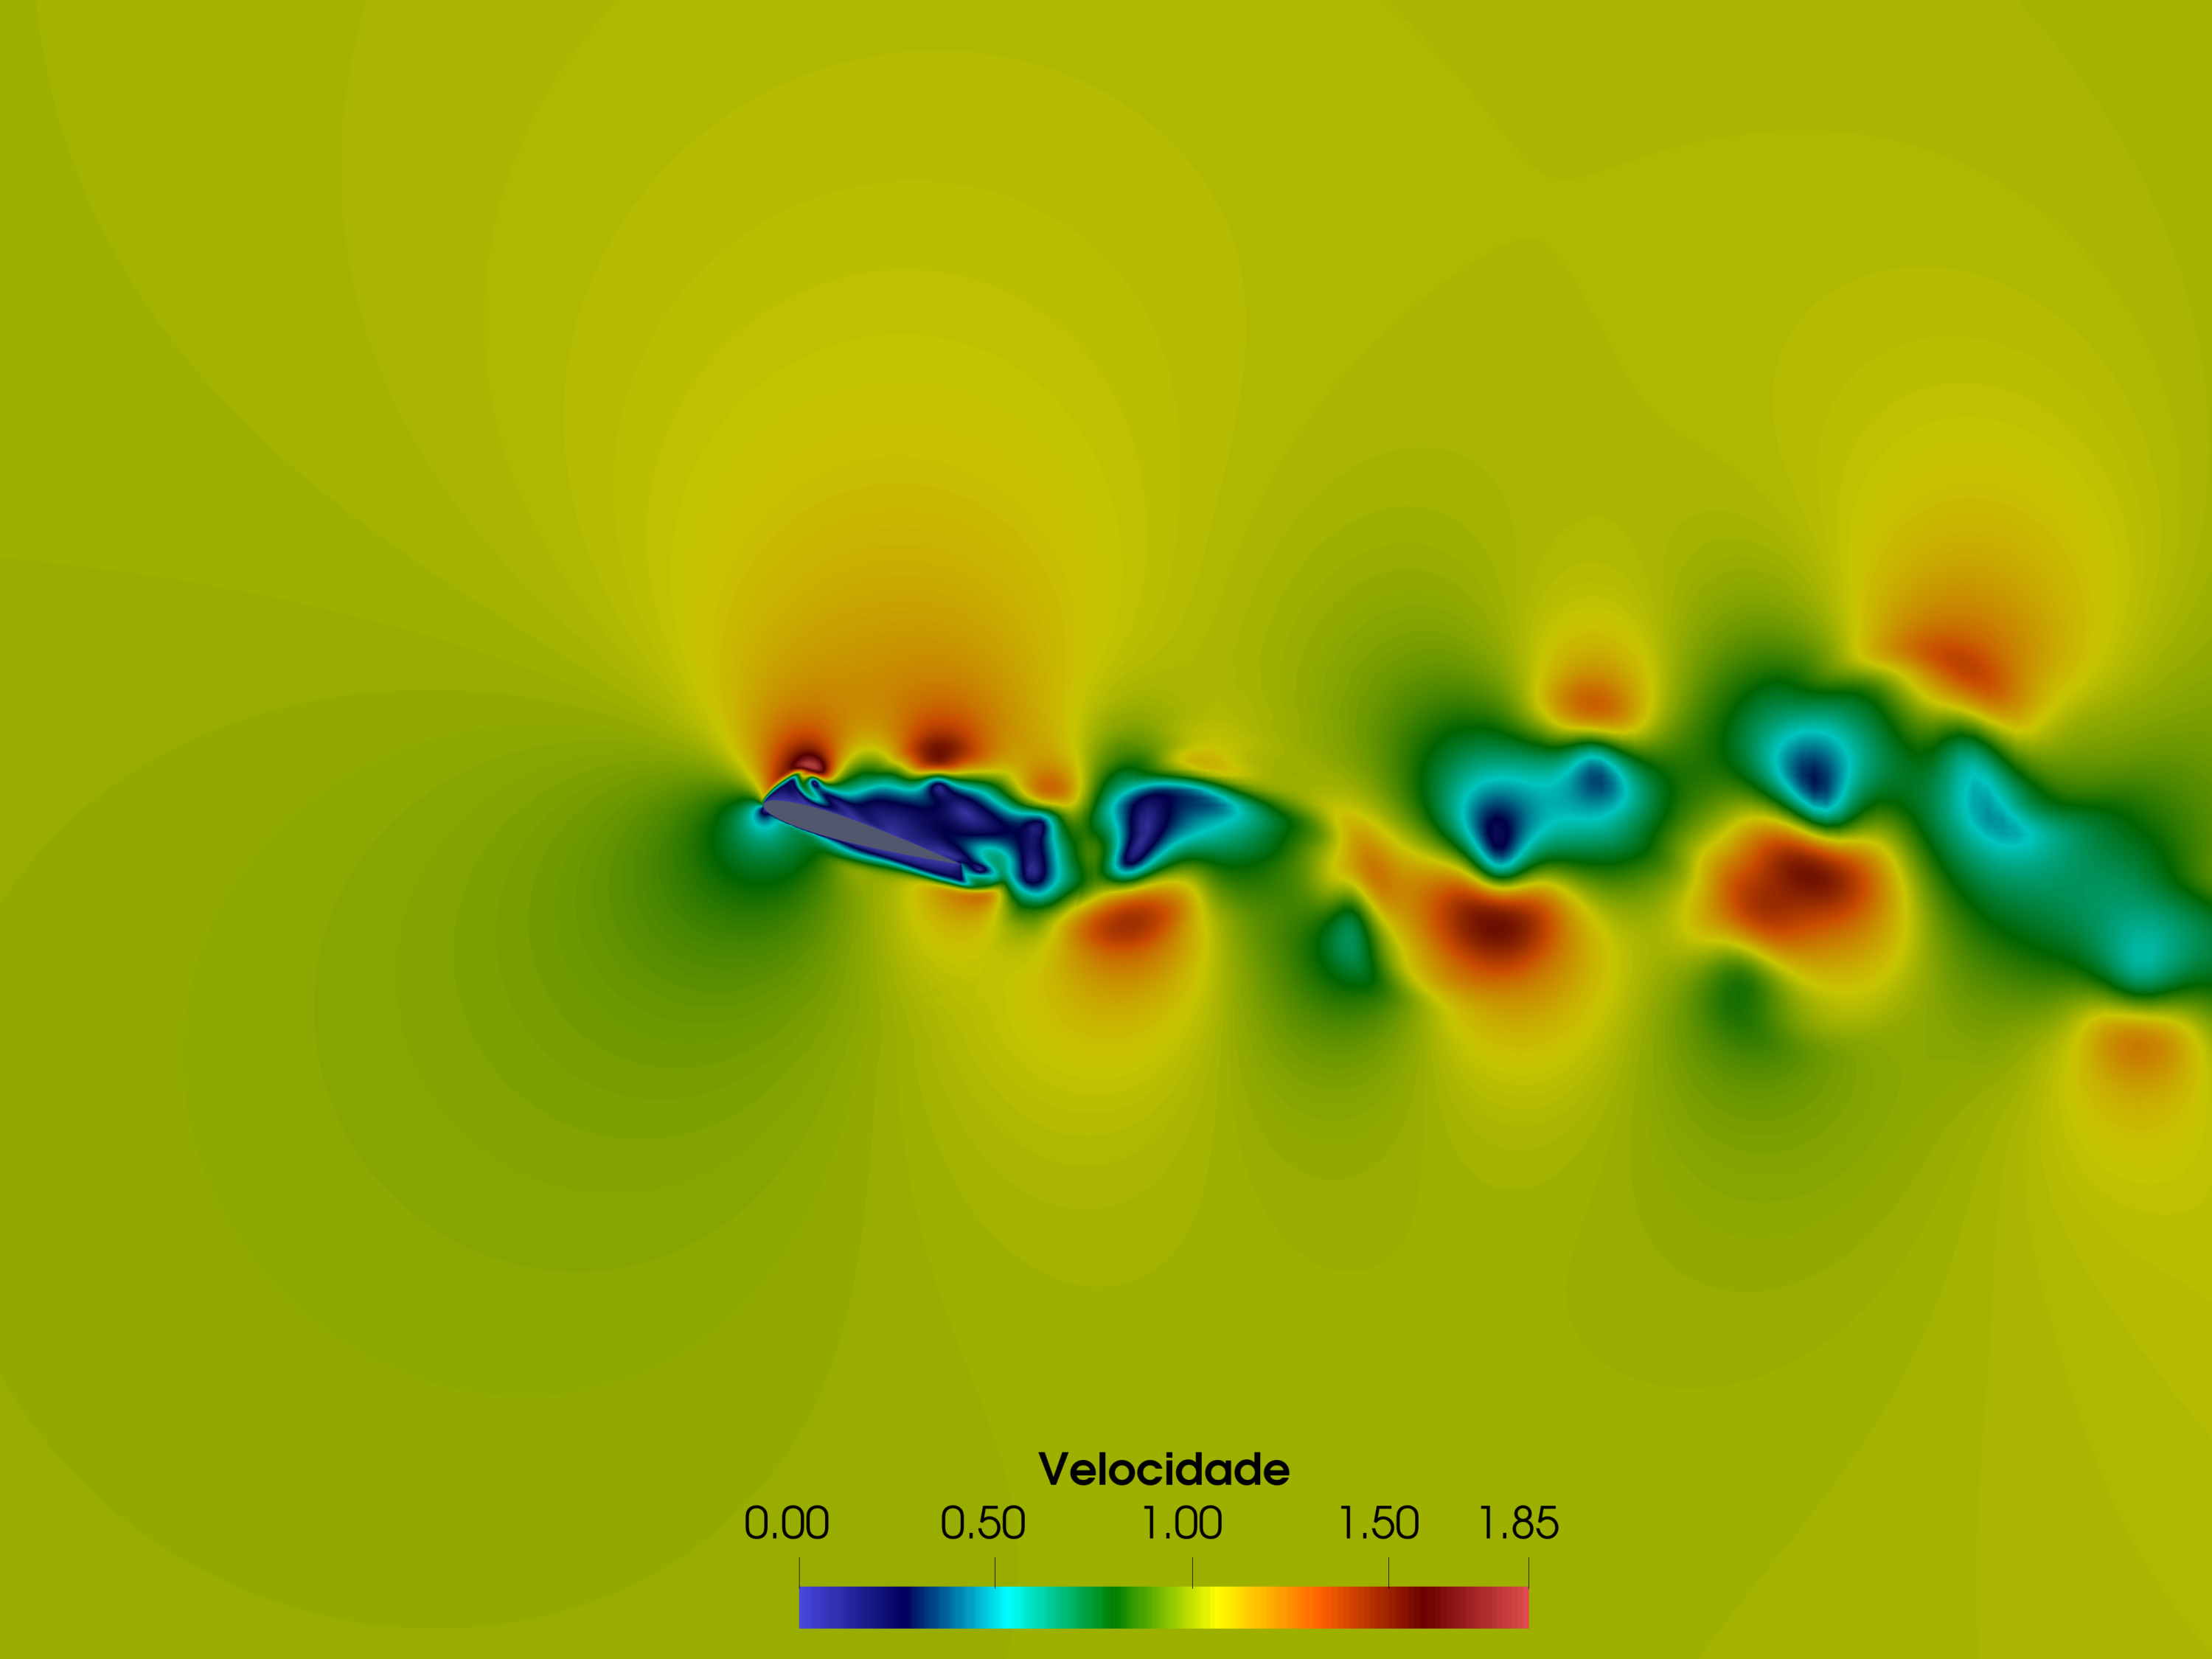
\includegraphics[trim=0 0 0 0,clip=true,scale=0.13]{Imagens/Cap6/aerofolioMov_vel440.pdf}}
	\label{fig:aerofolioMov_velocidade}
	\legend{Fonte: Elaborada pela autora}
\end{figure}

\begin{figure}[!htbp]
	\caption{Aerofólio Mov.: Campos de pressão}
	\centering
	\subfloat[$t = 8,0 $]{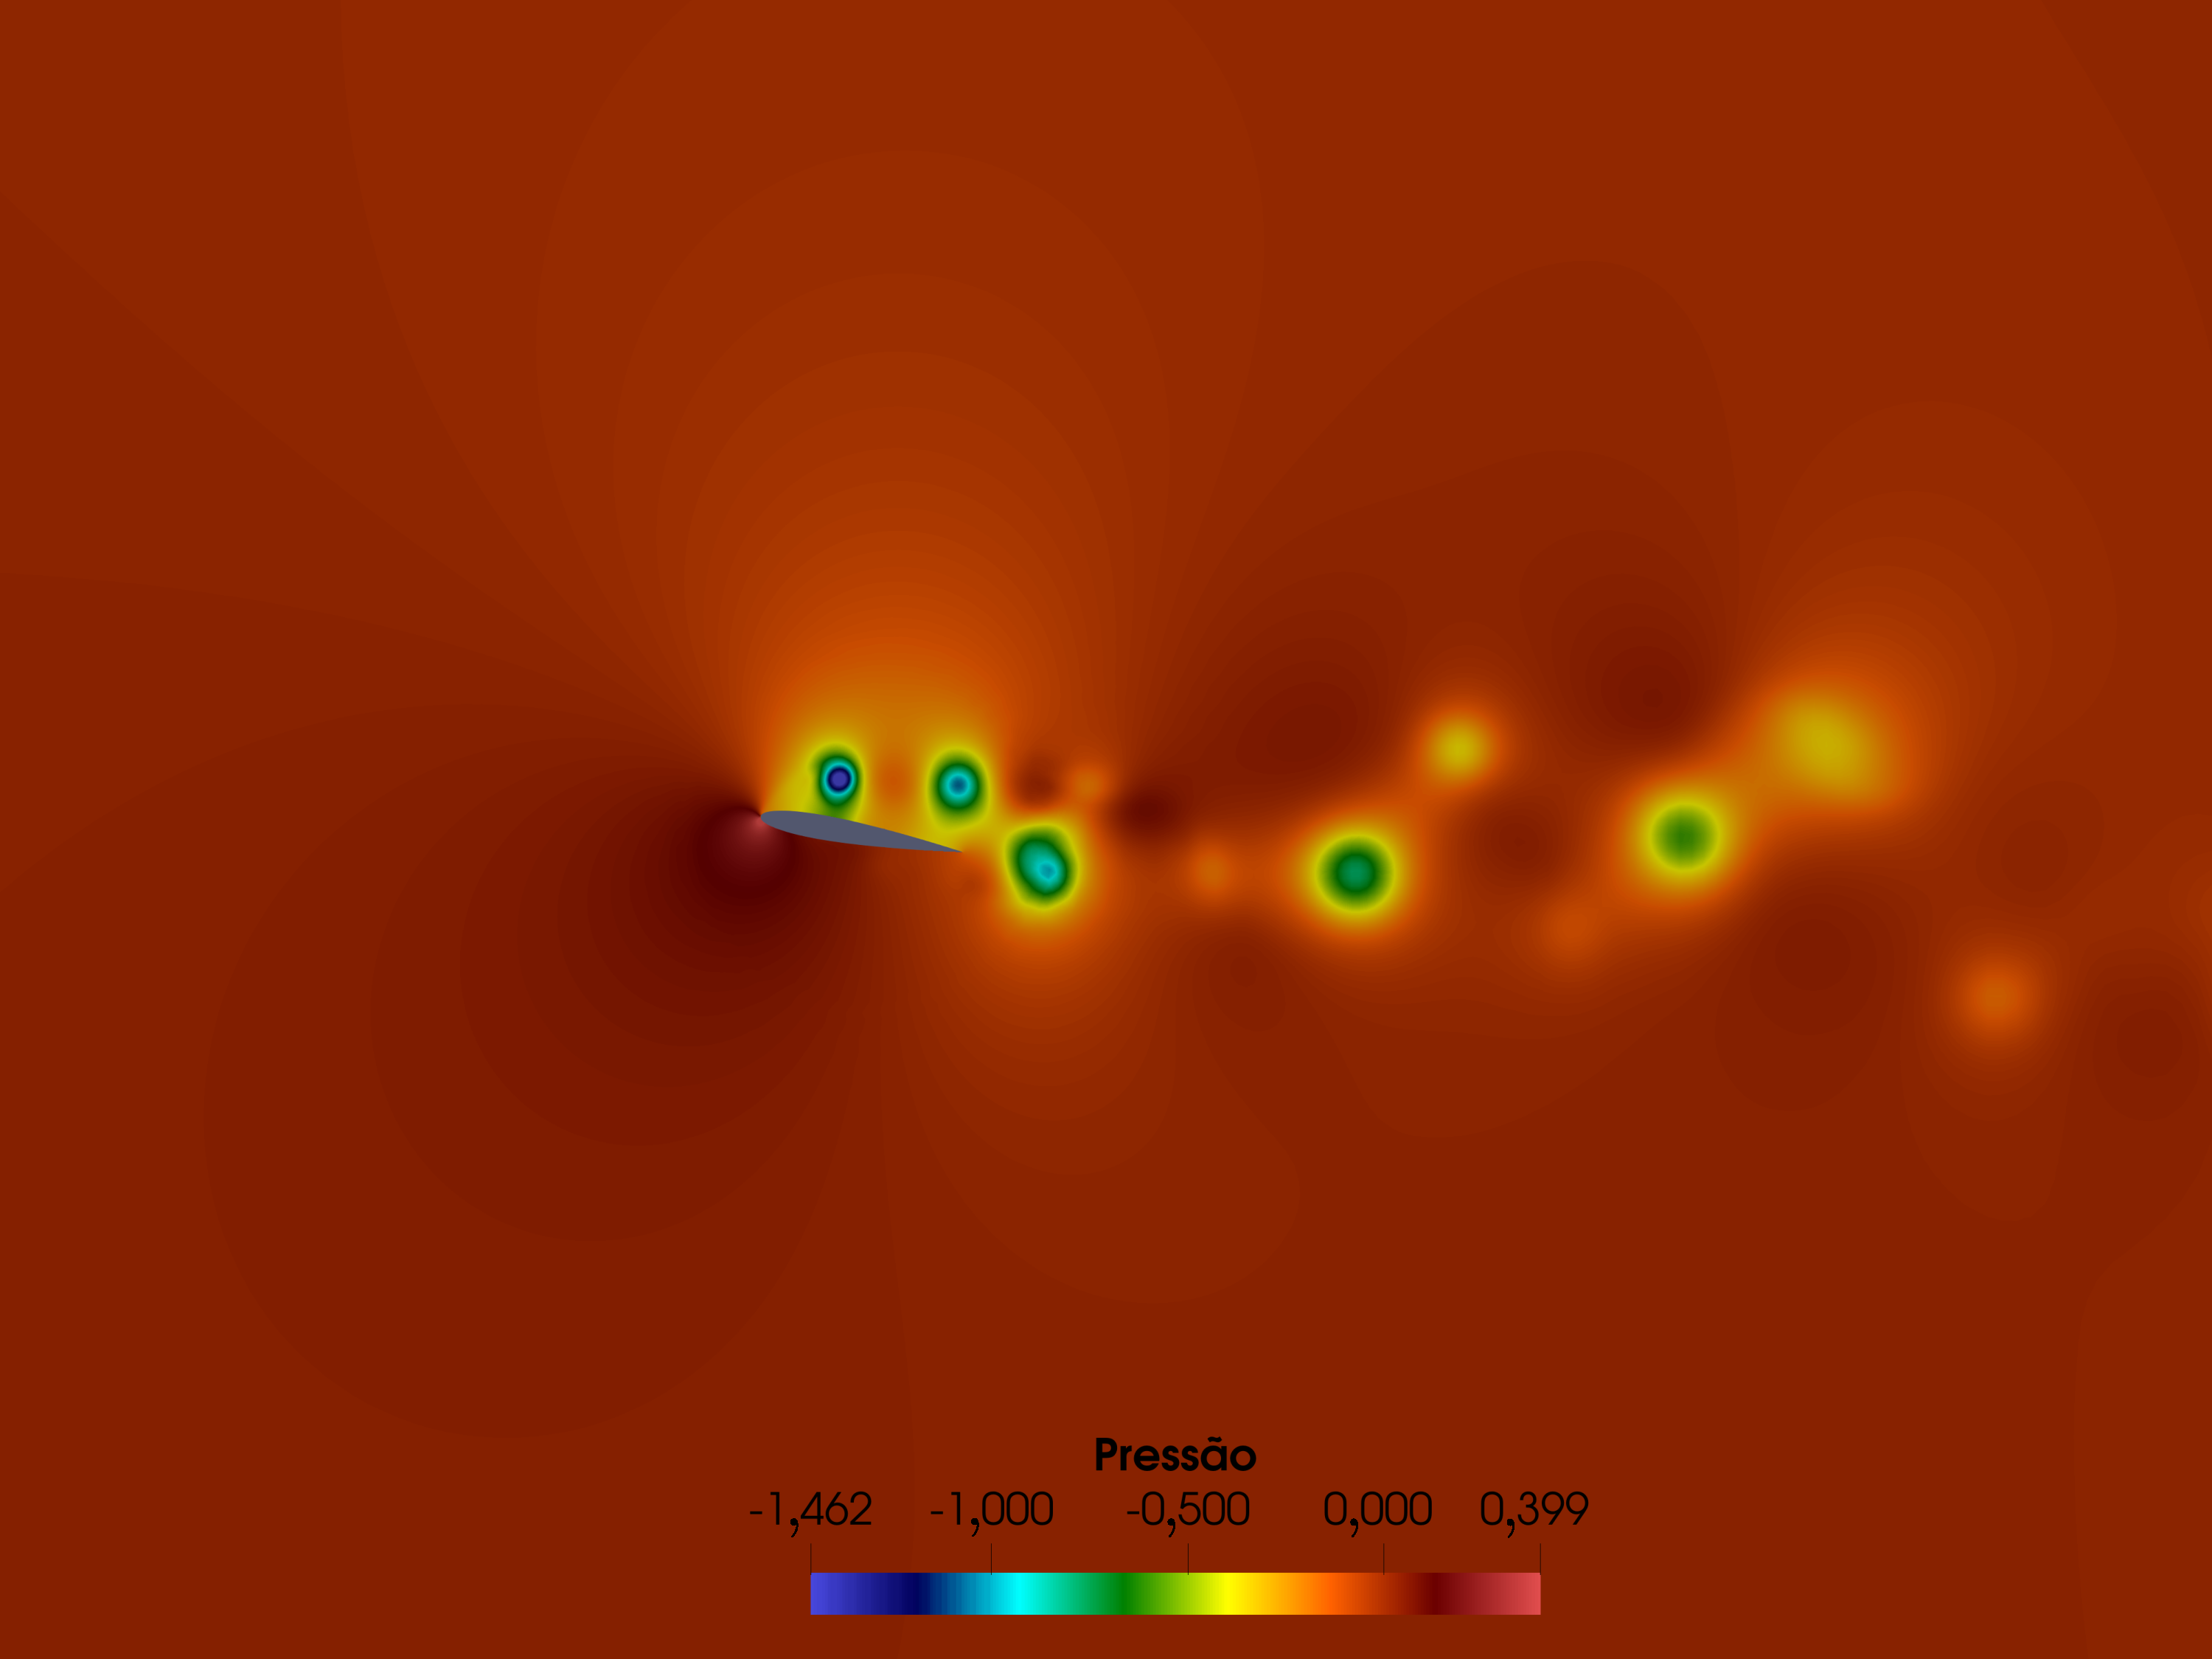
\includegraphics[scale=0.13,trim=0cm 0cm 0cm 0cm, clip=true]{Imagens/Cap6/aerofolioMov_press400.pdf}} \
	\subfloat[$t = 8,3 $]{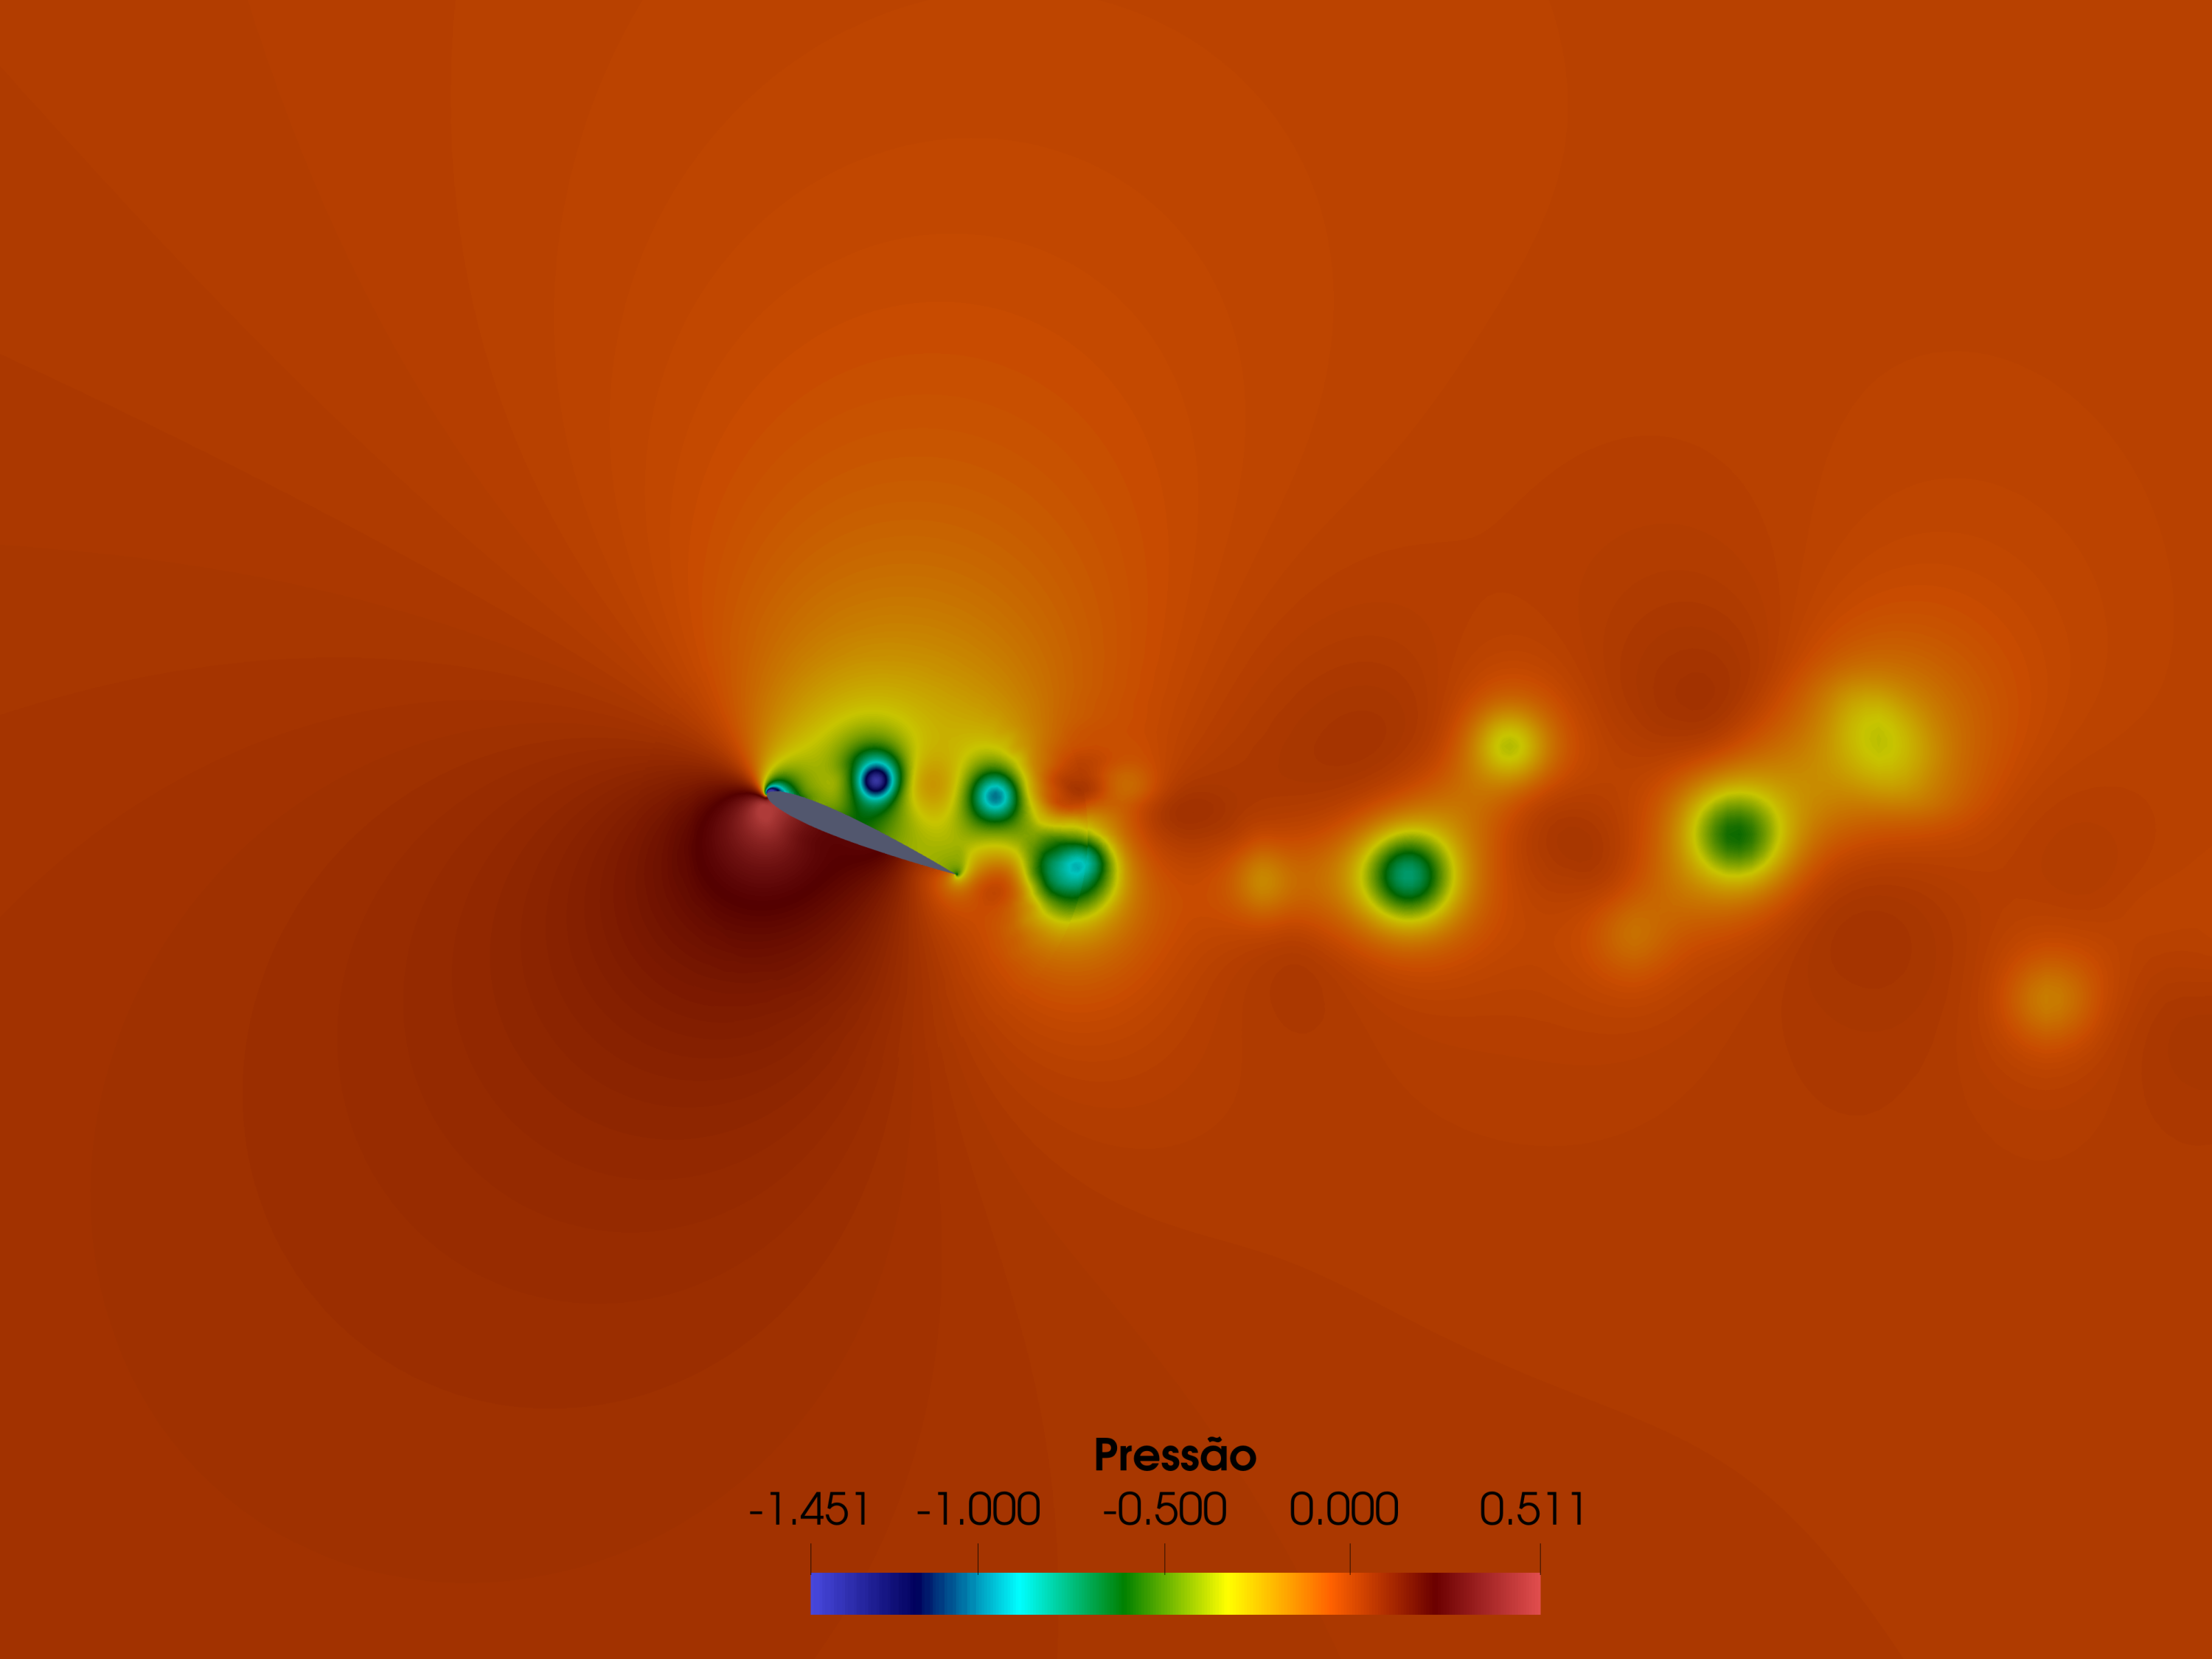
\includegraphics[trim=0 0 0 0,clip=true,scale=0.13]{Imagens/Cap6/aerofolioMov_press415.pdf}}\\
	\subfloat[$t = 8,5 $]{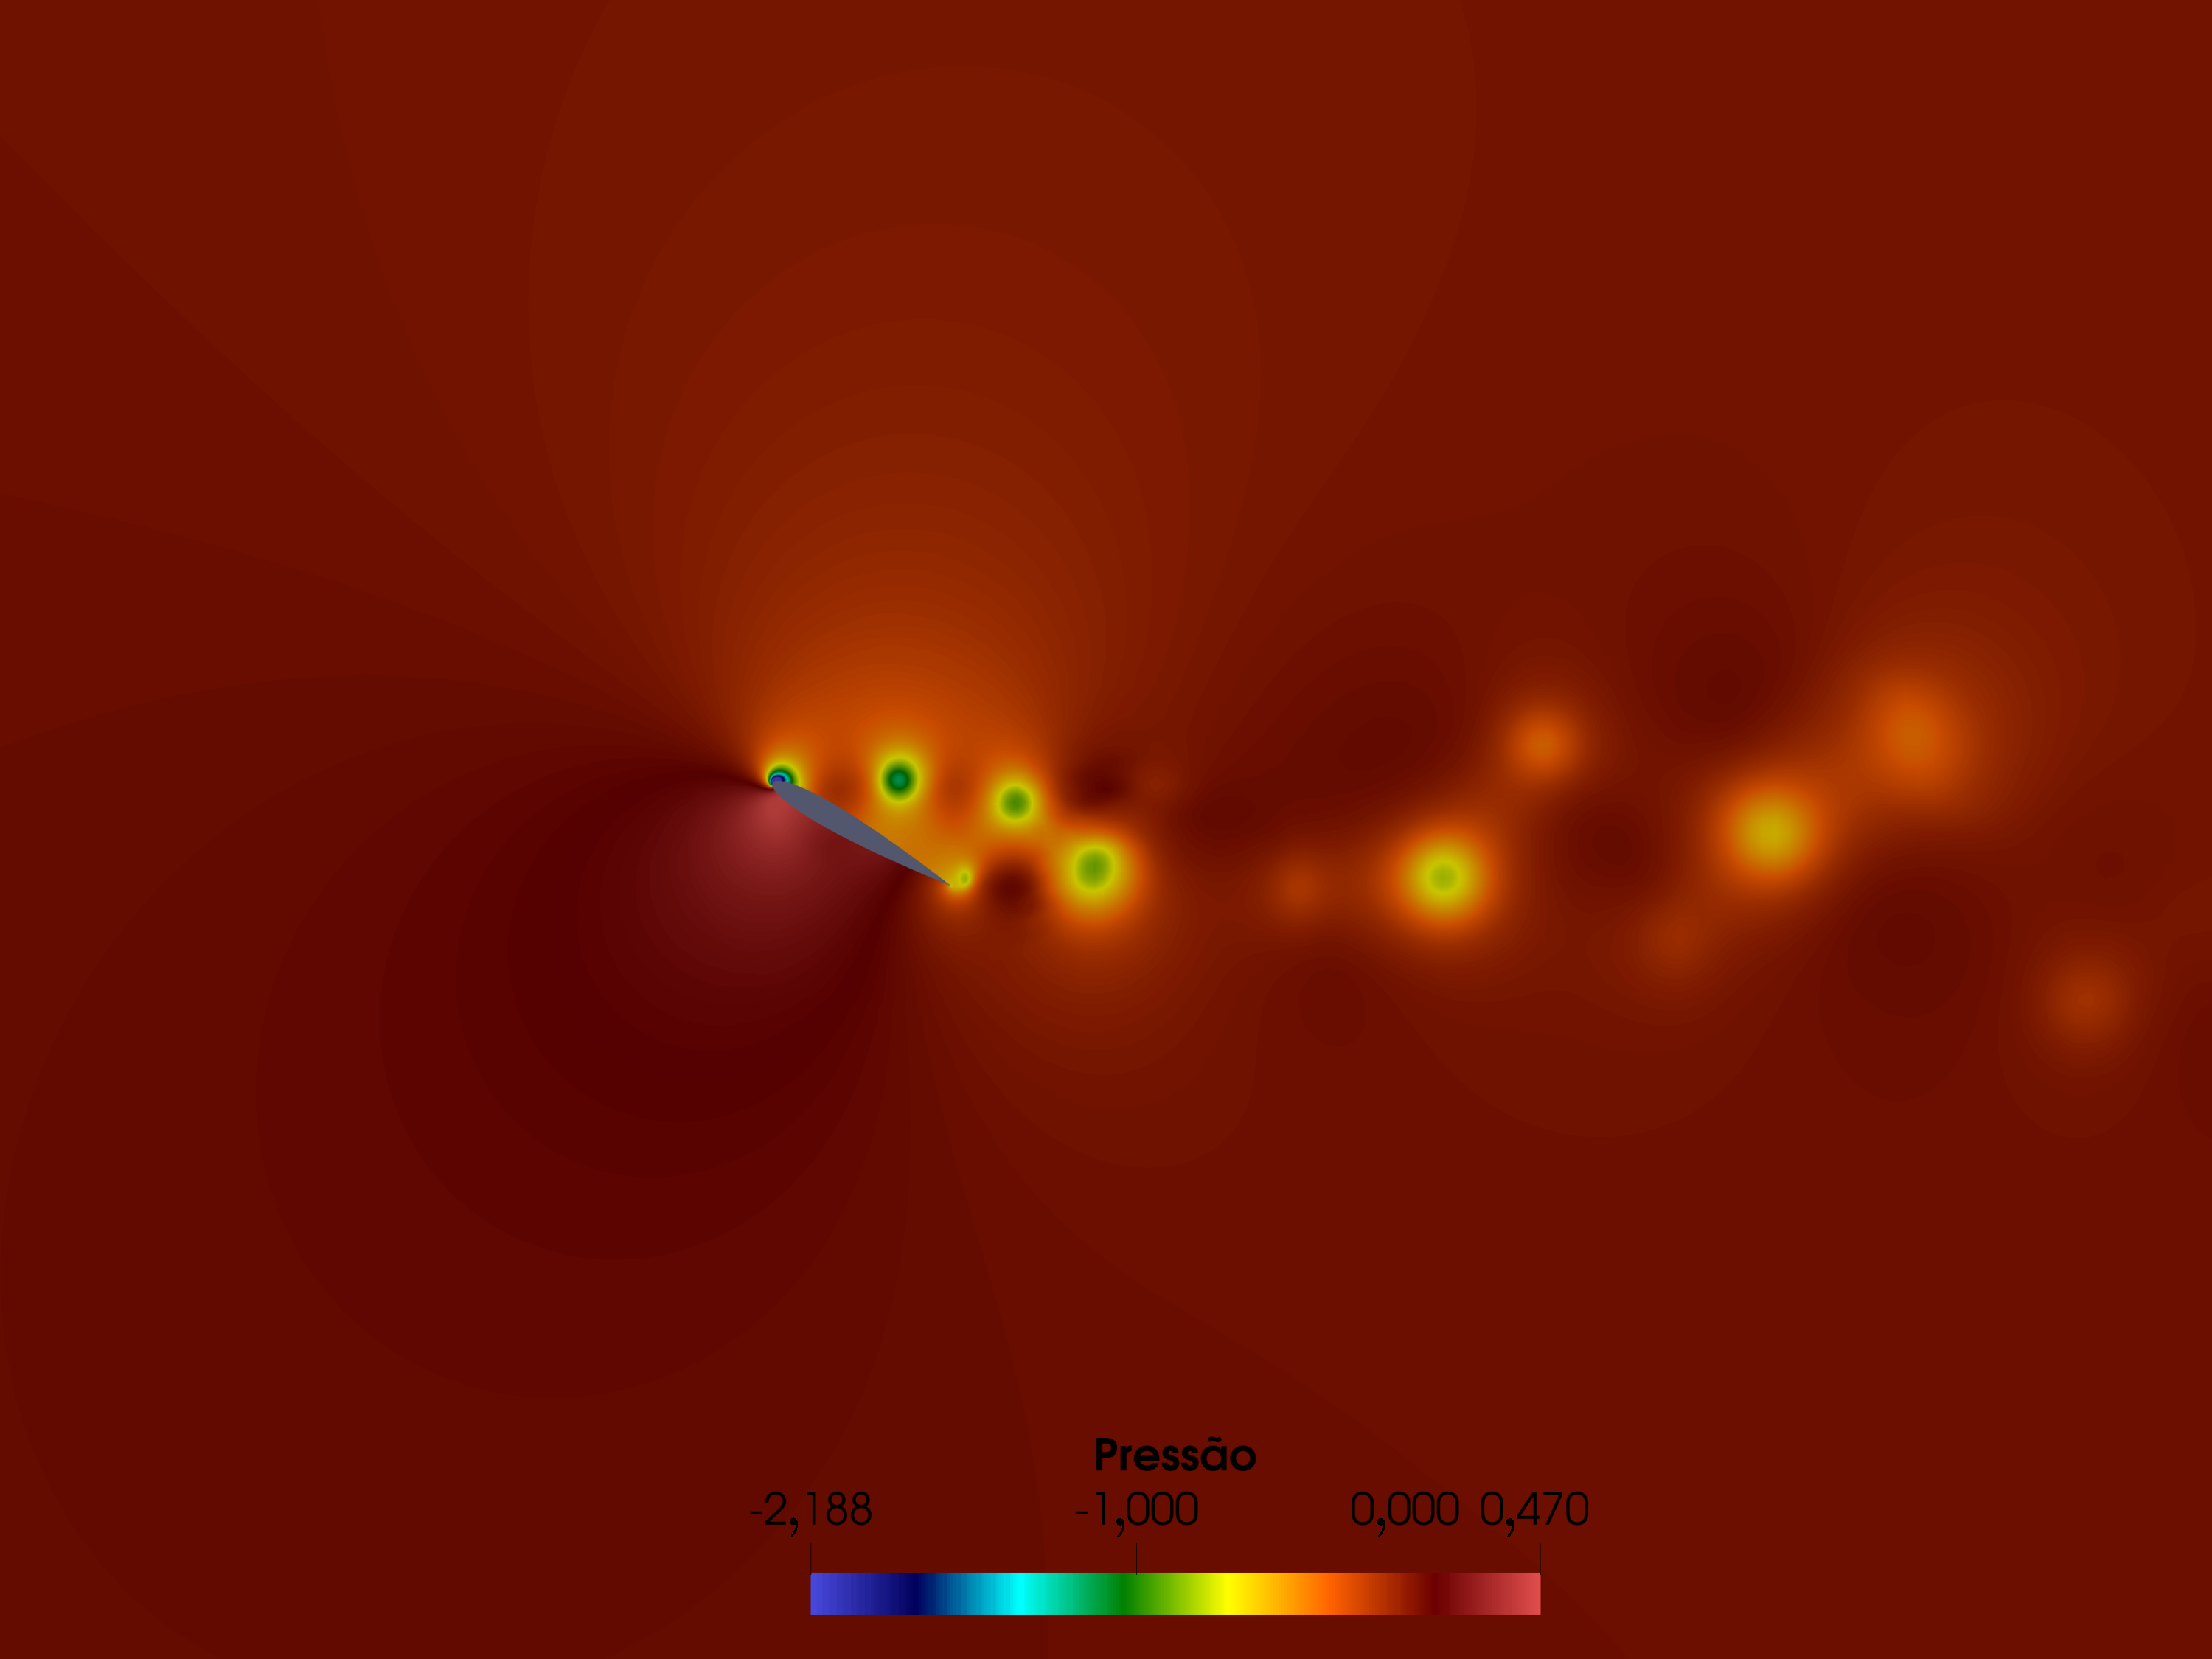
\includegraphics[scale=0.13,trim=0cm 0cm 0cm 0cm, clip=true]{Imagens/Cap6/aerofolioMov_press425.pdf}} \
	\subfloat[$t = 8,8 $]{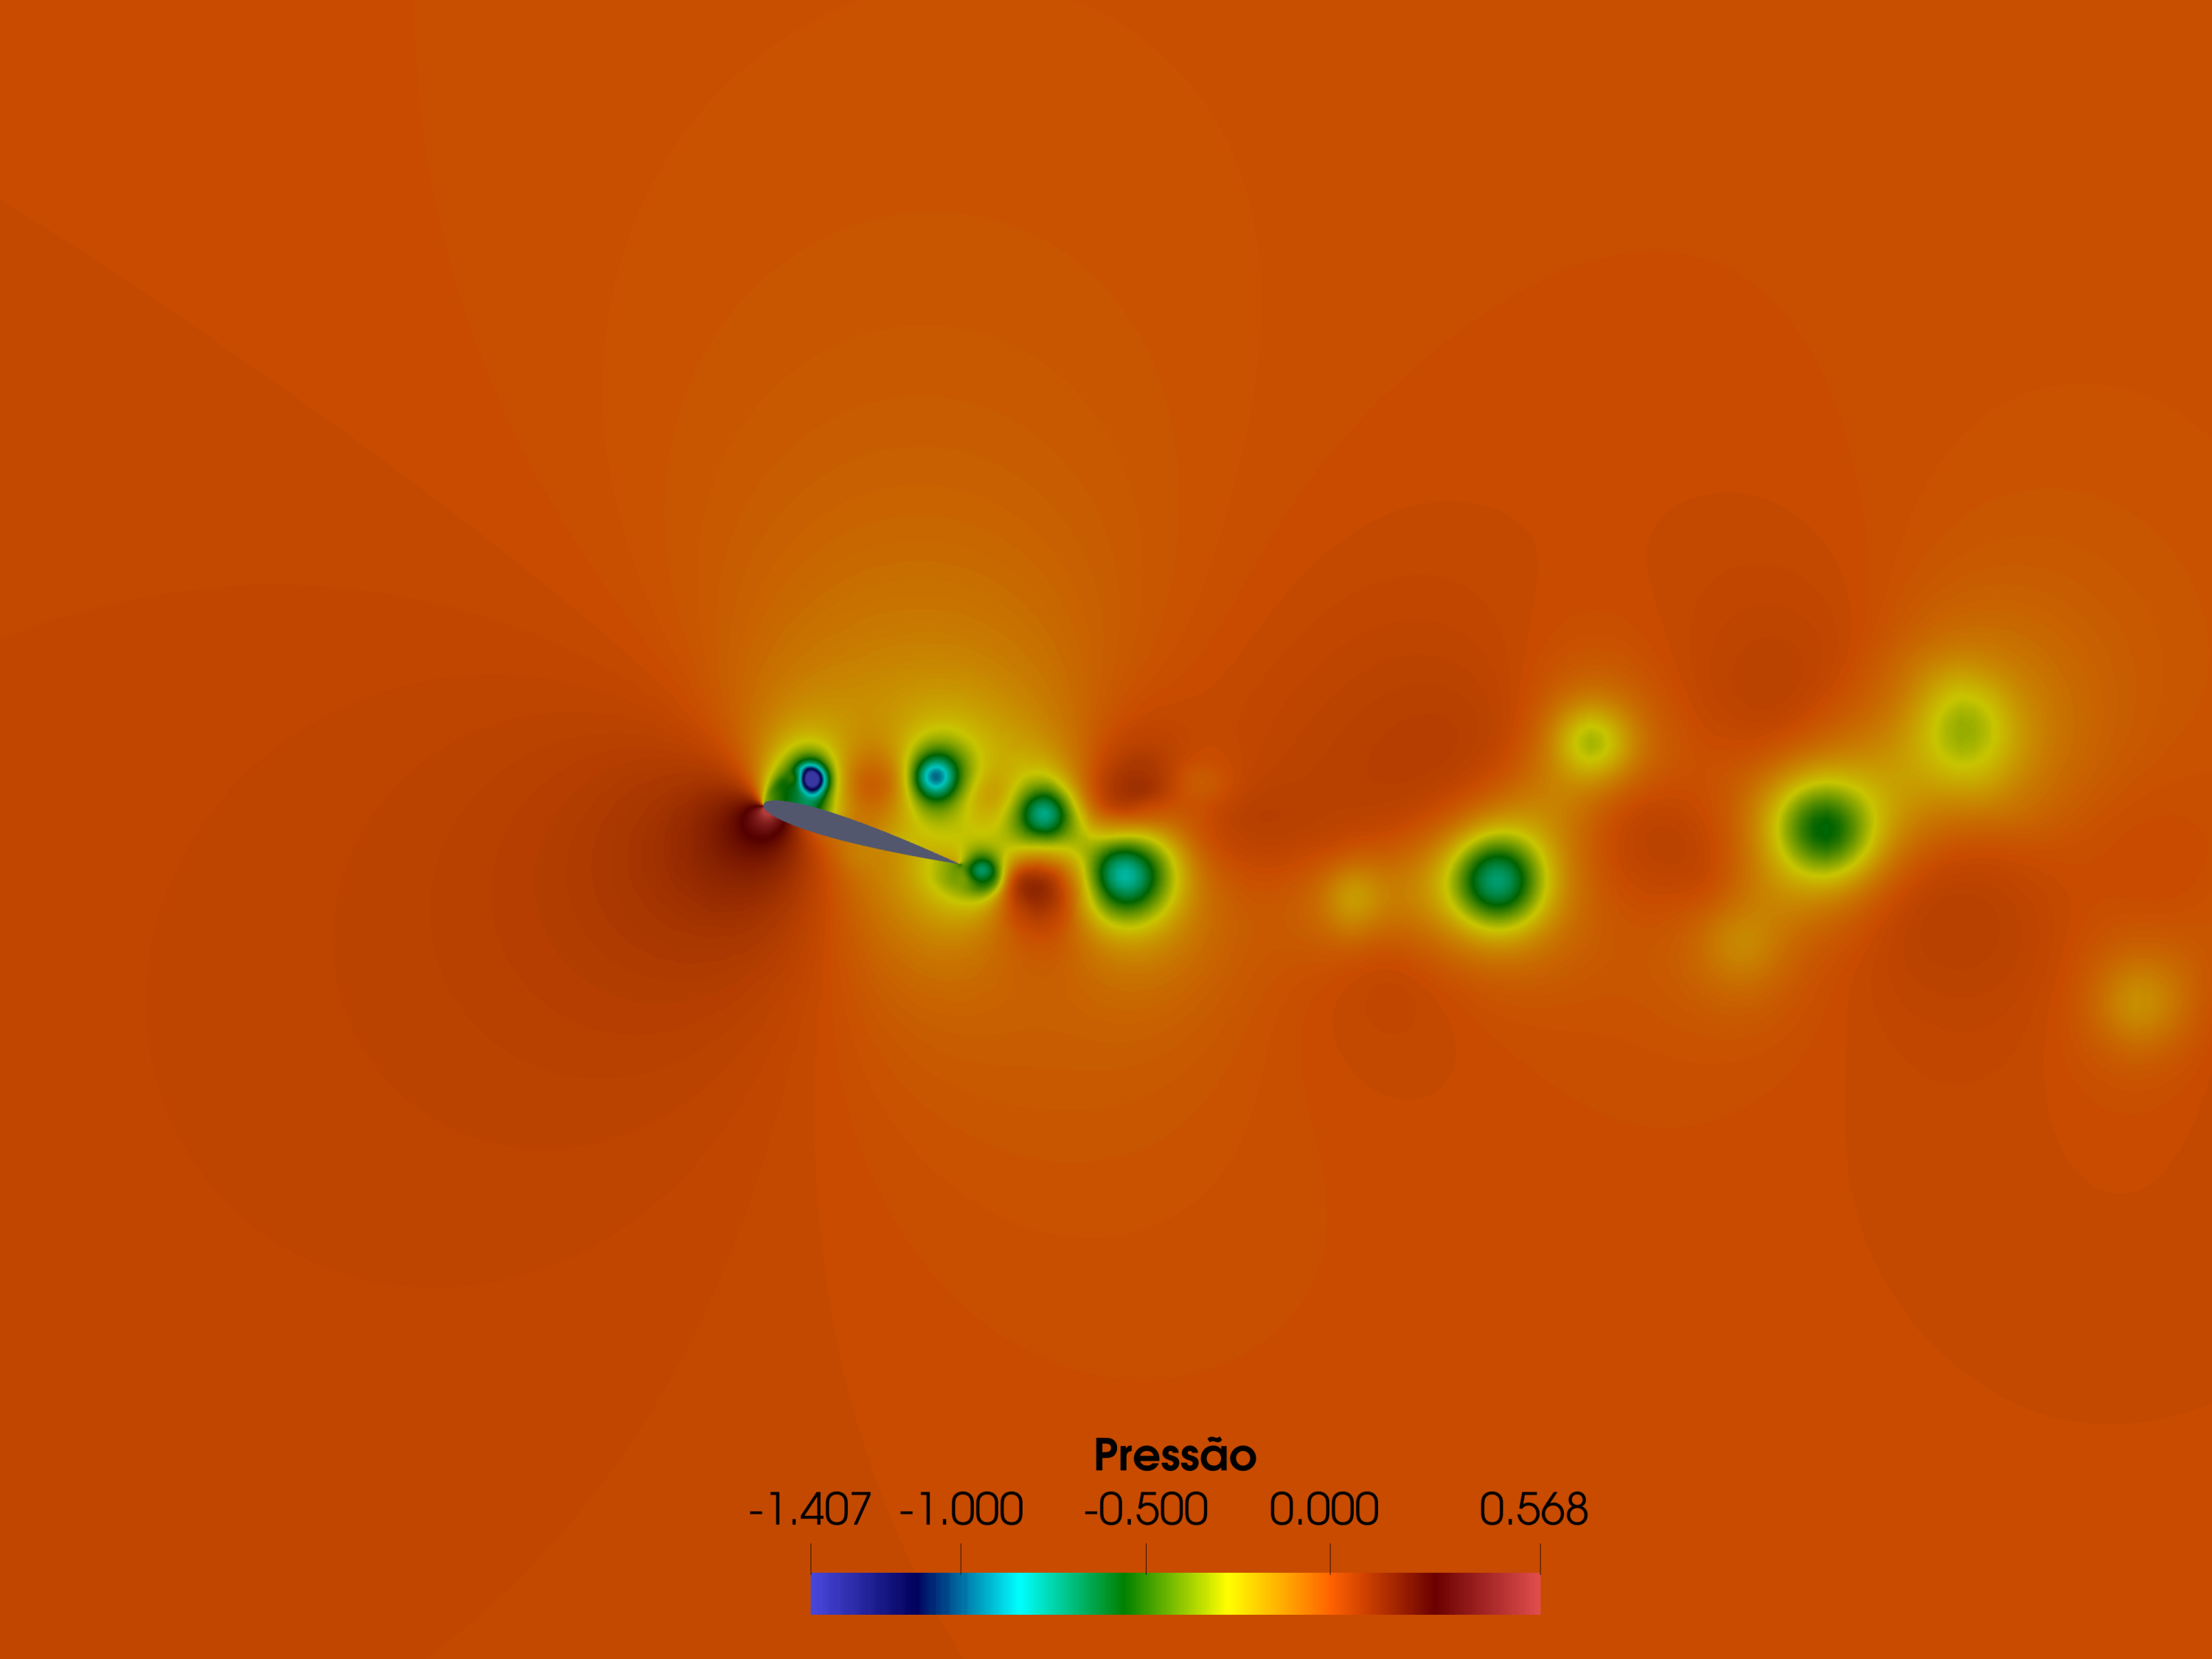
\includegraphics[trim=0 0 0 0,clip=true,scale=0.13]{Imagens/Cap6/aerofolioMov_press440.pdf}}
	\label{fig:aerofolioMov_pressao}
	\legend{Fonte: Elaborada pela autora}
\end{figure}
